\documentclass[openany,fontset=none]{intromech}

%\usepackage{showkeys}

\begin{document}

% 封面

\includepdf{body/F00-frontpage.pdf}

% 标题页

\includepdf{body/F01-titlepage.pdf}

% 出版信息页
% 出版信息页
\begin{center}
    \zihao{4}\fangsong \mbox{}

    \mbox{}

    责任编辑:张晓红

    封面设计:陈治黄

    \vfill \heiti 力~~学~~概~~论

    \normalsize \kaishu 方励之~~李淑娴

    \normalfont *

    安徽科学技术出版社出版

    \zihao{-5} (合肥市跃进路1号)

    \normalsize 安徽省%
    \hspace{0.2em}\raisebox{-0.5mm}{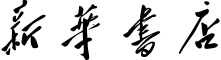
\includegraphics[width=4em]{icon/xinhuabokestore}}\hspace{0.2em}%
    发行~~安徽新华印刷厂印刷

    *

    \zihao{6}开本:850$\times$1168~~1/32~~印张:12.5~~字数:309,000

    1986年1月第一版~~~~1986年1月第一次印刷

    印数00,001—5,000

    \normalsize 统一书号:13200$\cdot$68~~~~定价:2.5元
\end{center}
\thispagestyle{empty}
\clearpage


% 内容提要
% 内容提要
\begin{center}\begin{minipage}{8.4cm}\vspace{3cm}
        \begin{center}\heiti 内~容~提~要\end{center}
        \normalfont \zihao{-5}
        \hspace{2em}本书是根据作者在中国科学技术大学及北京大学讲授普通物理的
        力学部分讲稿整理而成的。其特点是强调用物理的前沿发展去改进基础物理教
        学,即用现代物理的观点去选择课程的内容,去表现概念和规律。因此,书中
        包括一些在传统的教材中没有的内容,如牛顿宇宙学等,对许多传统的内容,
        也采取新的讲授法,使之能与当代物理的进展相呼应。另外。由于力学是物理
        学的入门和基础,所以本书也注意物理方法的阐述,这对于初学物理的学生是
        有益的。书中还附有一些习题及答案。

        \hspace{2em}本书可作为综合大学及师范院校的普通物理力学教材,也可供大
        专院校物理教师及物理教学研究工作者参考。
\end{minipage}\end{center}
\thispagestyle{empty}
\clearpage

% 序言
\setcounter{page}{1}
\pagestyle{foreword}
\null\vspace{1em}
\begin{center}
    \zihao{4}\heiti 序

    \null
\end{center}
\fangsong \normalsize

这本书原是一份普通物理课程的力学讲义,它曾在中国科学
技术大学沿用多年,也曾在北京大学教授过数次。

普通物理中的力学,是相当难教的,凡是教授过这门课的老
师,大都有此体会。一方面,力学是整个物理学的基石,它包含
许多基本的观念、方法和理论,需要学生极为准确地加以掌握,
以备后继学习之用,另一方面,初入大学的学生,往往看轻力学,
误认为新的内容不多,似乎在中学里都已学过,结果力学反而被
疏忽了。

这种局面迫使一些教师采用理论力学的方法来教授普通物理
力学。这样做,确实可以解决前述问题的第二方面,学生不再感
到“似曾相识”了。随着教和学二者的提高,原属理论力学的部
分内容的确可以逐渐放到普通物理中来。但是,我们觉得,若仅
限于这一途径改进教学,还不能或不完全能解决问题的第一个方
面——力学是整个物理的一块基石。

基石到底在哪里起了基石的作用?基石到底如何起了基石的
作用?显然,这些“哪里”,这些“如何”只有从物理的当代发
展以及前沿研究的角度,才能看得清楚。这就是说,如果我们企图
从“物理的基石”这一标准来组织教学,它至少有以下两方面的
含义:一是不断用新的现代的观点去整理老的内容,一是不断用新
的前沿的重要成果来充实基础。事实上,不同时代的教材的差别,
最清楚地表现在这些方面。上进的标准,也就是我们在编写这本
教材时,尝试着击追求的。也许有的地方达到了,也许有的地方%分页处
并未达到。无论成功或失败,它都是我们的追求的记录。

为了使用上的方便,书中编辑了一些例题,每章末也附有一
些思考题和习题。由于北京大学物理系和中国科学技术大学物理
教研室已编有《物理学习题集》(人民教育出版社,1980),为了不
重复太多,本书中的例题和习题只是标志性的。在教学上需要更
多习题时,可以参考上述的习题集。

在使讲义变成这本书的过程中,得到过员汝槐同志的协助,
谨致谢意。

~

\hspace{6.8cm}\zihao{-4}\kaishu 作~~~者

\mbox{}

\hspace{7cm}\normalfont \zihao{-5}1984年4月\normalsize
\clearpage

% 目录
\clearpage
\setcounter{page}{1}
%\tableofcontents

% 正文
\clearpage
\pagestyle{heading}
\setcounter{page}{1}
% 公式与上下文本距离调整
\setlength\abovedisplayskip{1pt plus 3pt minus 1pt}
\setlength\belowdisplayskip{1pt plus 3pt minus 1pt}

% 绪论
\chapterx{——物理世界的统一}\label{chp:00}

物理学的兴起,是从经典力学开始的。在经典力学之前,人类
的文明中虽然已有不少具有物理价值的发现和发明,但是并不存
在一门独立的物理学。因此,我们在学习经典力学的时候,首先
应当了解:为什么经典力学成了物理学的起点?经典力学在整个
物理学中占据着怎样的地位?

爱因斯坦曾经这样来概括牛顿力学的历史地位;“古代希腊
伟大的唯物主义者坚持主张,一切物质事件都应当归结为一系列
的有规律的原子运动,而不允许把任何生物的意志作为独立的原
因。而且无疑笛卡尔曾按他自己的方式重新探索过这一问题。但
是,在当时,它始终不过是一个大胆的奢望,一个哲学学派的成
问题的理想而已。在牛顿之前,还没有什么实际的结果来支持那
种认为物理因果关系有完整链条的信念。”

这句话的意思是,物理学依赖于一种基本的信念:物理世界
存在着完整的因果链条,即自然界是统一的。牛顿力学则是体现
这种信念的第一个成功的范例。

从牛顿力学的创建到现在,已经有三百多年了,物理学已经
大大发展了,远远超过了经典力学原有的水平。但是,就物理学
的最基本的追求和物理学的总目标来说,却一直没有变化。经典
力学时代的追求和目标,可以说时至今日仍然是整个物理学的追
求和目标。这个最基本的追求和目标,就是自然界的统一。的确,
从整个物理学的发展中,可以看到一条鲜明的主线。这就是执着%分页点
地追求宇宙的统一,找寻支配宇宙万物的最基本最统一的规律。

相信存在统一,努力寻求统一,如果仅仅作为一种自然观,
早在古代已经有了。老子的《道德经》中写有:“道生一、一生
二、二生三、三生万物。”这就是中国古代的一种统一观,它完
全可以与爱因斯坦所提及的古希腊的哲学相媲美。不过,无论在
古代中国或古希腊,统一观都只是一种哲学思辨。

牛顿的力学和古代的哲学不同,它不是思辨地坚持统一观,
而是发展了寻找统一的有效的物理方法。牛顿在他的最重要的力
学著作《自然哲学的数学原理》中阐明了他采用的方法。他在前
言中写道;“我奉献这一作品。作为哲学的数学原理,因为哲学
的全部责任似乎在于——从运动的现象去研究自然界中的力,然
后从这些力去说明其他的现象。”\sbfootnote{牛顿这段话里的
    “哲学”一词,实际含义相当于今天的“科学”或“物理学”。}这就是
说,寻求统一的出发点不是思辨而应是运动现象。自然界中的运动
现象是多种多样的,物理学的责任就在于寻找支配这些现象的统一的力。

今天的物理学,仍然大体地沿袭着牛顿所开创的研究途径。
寻找统一的力,或统一的相互作用。因此,几乎所有基本的物理
理论都称做某种力学,如牛顿力学、电动力学、色动力学等等。
每一种新的力学的确立,都标志着我们在追求统一的逾程上达到
了一个新的水平。

为了更具体地表达上述的论述。我们利用表1。表1左边列举
的是自然界中的种种运动现象,也就是物理学的研究对象。天体
的运行和地面物体的运动是人首先看到或接触到的,随后才有时
间、空间的概念,所以时空也是一种物理研究的对象,另一类现
象是电、磁和光,所有这些物理对象。在二十世纪之前,人们都
已知道了。二十世纪以来,又逐渐证实或发现一些新的对象。如
原予、原子核、核子以及夸克等。

表\ref{tab:00.01}~的其余部分就表示物理学在寻求统一,寻求完整的因果
链条上一些重要的阶段。
牛顿的力学和万有引力定律,是物理学上第一次大的统一。
在牛顿之前,传统的观念认为支配天体运行和支配地面物体运动
的规律是不相同的,有所谓天界和世俗两个世界之分。然而,牛
顿发现,天上行星和月亮的运动,实际上和地面落体运动遵从相
同的规律,它们都是由引力引起的。这样,牛顿就用他的力学打
破了天界和世俗的界限,找到了两个世界的统一。牛顿称引力为
万有引力,就是强调这种统一。

第二次大的统一,是由十九世纪的麦克斯韦完成的。他建立
了电磁理论,使电、磁及光学现象得到统一。这就是电动力学。

很快发现,牛顿的力学和麦克斯韦的电磁学这两大领域在时
\begin{tablex}[!h]
    \centering
    \caption{物理学发展中的统一$^*$}
    \label{tab:00.01}
    \begin{tabular}{c}
        \toprule \vspace{-1em}                                      \\
        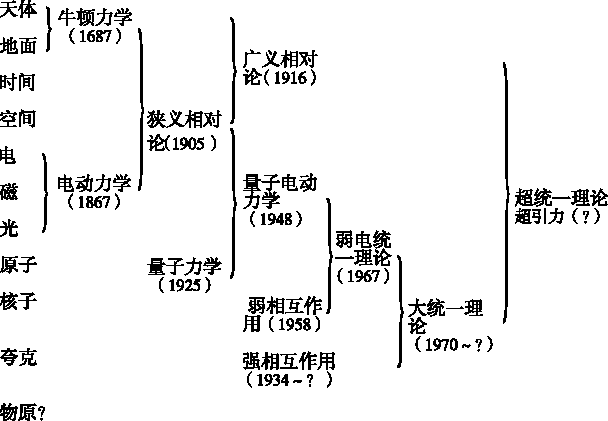
\includegraphics[width=0.98\linewidth]{figure/tab00.01} \\
        \bottomrule
        \zihao{6}* 括号中的数字表示相应的理论建立的年代;有问号的表示尚未完成。
    \end{tabular}
\end{tablex}
空观上是很不协调的。在前者中,各种匀速运动是平权的,但却
假定有绝对空间或绝对速度存在。相反,在后者中,有一个地位
特殊的速度,即光速,但却始终测不出这个特殊的速度是相对于
哪一个绝对空间而言的。爱因斯坦抛弃了绝对空间观念,使电磁
学、力学在新的时空观的基础上达到了协调和统一。

爱因斯坦还曾企图把引力和电磁力二者统一起来,但他的努
力没有成功。然而,他却找到了能与麦克斯韦电磁理论相协调的
引力理论——广义相对论。

作为引力理论的广义相对论和作为电磁理论的麦克斯韦理论
构成了我们今夭称为经典物理学的理论基础。

与经典物理相对的是量子论。量子力学最初是作为原子、分
子的统一的力学而发展起来的。这种新的力学统一地解释了原子、
分子的各种光谱现象,统一地解释了元素周期表,统一地解释了
各种不同分子的键合。

在将量子力学扩展到电磁场时,遇到了困难,这本质上是由
于电磁场是相对论性的。直到四十年代末,发展了所谓重整化方
法才巧妙地解决了上述的困难,使量子论与电磁理论能得以统一,
产生了量子电动力学。

到六十年代末,我们已经得到了如下的物理世界的图象。宇
宙中的所有物理对象可以分成两大类,一类称为“物质”,如夸
克、电子、$\mu$子等等,另一类称为“相互作用”,如引力、电磁力
等等。在目前的宇宙中,有四种基本的相互作用,按它们的强度
顺序排列是:核子参与的强相互作用,荷电粒子参与的电磁相互
作用,核子及电子、中微子参与的弱相互作用,以及任何粒子都
参与的引力相互作用。可以简单地说,宇宙间的一切运动和变化。
都可以统一为这四种“力”的作用。但是,追求统一的物理学,
似乎认为这种状况仍然不够统一。

1967年,温伯格和萨拉姆再次着眼于统一,先后提出了电磁
相互作用和弱相互作用的统一理论。随后的一系列实验证明他们
的统一理论是正确的。

这一新的成功,促使许多人去找寻把电磁作用、弱作用及强
作用都包含在内的统一理论,通常称为“大统一理论”。建立这
种理论的工作还没有完成,这是正在研究的领域。

如果大统一能够顺利完成,下一步的统一就是要把引力也统
一在内了。引力是物理学最早讨论的一种基本的力。但是,它与
其他力的统一最难,因为引力有一系列很特别的性质。例如这种
力只有引力却无斥力。就是这种特别性质之一。

企图把引力与其他力统一起来的工作,称为超统一的研究。
目前还没有得到有实际意义的结果。它是今天的物理学的一个前
沿。实现超统一的一个可能是用超引力理论,这种理论中的统一
有一个很有趣的特点,即它把物理学中传统的“物质”与“相互
作用”之间的界限也打破了。

总之,从牛顿力学开始,物理学就在寻找宇宙的统一,我们
希望找到控制着万事万物运动的极少的几个基点。只有从这个角
度我们才容易看清经典力学在整个物理学中的地位和作用,也才
能全面地了解学习经典力学对于学习整个物理学的意义和作用。


% 第一章
\chapter{时间,空间和运动学}\label{chp:01}

\section[时间]{时~~~~间}\label{sec:01.01}

描写物体的运动,要用时间和空间这两个概念。因此,我们
先来对时间、空间本身作一些分析。

时间和空间可以说是最平凡的概念了,因为在日常生活中也
常常用到它们。不过,若问什么是时间?什么是空间?却又不容易
找到恰当的答案。其实,这是两个很难的问题。尽管有不少关于
时间和空间的定义,但大都不能令人满意。一种或许可以接受的
说法是:时间、空间是物理事件之间的一种次序,时间用以表述
事物之同的顺序,空间用以表述事件相互之间的位形。

没有满意的“严格”的理论定义,并不妨碍时间和空间二者
在物理中的使用。因为,物理学是一门基于实验的科学,在考查
物理学的概念或物理量的时候,首先应当注意它与实验之间是否
有明确的、不含糊的关系。对于时间和空间这两个基本概念来说,
首要的问题似不是去追究它们的“纯粹”定义,而是应当了解它
们是怎样量度的。

量度时间,通常是用钟和表。然而,钟和表并不是测量时间
的唯一的工具。原则上。任何具有重复性的过程或现象,都可以
作为测量时间的一种钟。自然界里有许多重复性的过程,其中有
一些我们早已把它们当作计时标准了。例如,太阳的升没表示天;
四季的循环称作年;月亮的盈亏是农历的月。其他的循环过程,
如双星的旋转、人体的脉搏、吊灯的摆动,分子的振动等等,也
都可以用作测时的工具。

更一般地说,只要知道了某个物理现象随时间的变化,尽管
它不是重复性的过程,也可以用来测定时间。譬如,我们能从一
个人的容貌估计出他的年龄,因为容貌这个量与时间之间有确定
的关系。这个例子虽然很普通,但某些有用的测时方法与此是很
相似的。在确定星体的年龄时,常常就是根据星体的颜色。

钟的种类很多,但有好有坏。比较两个人的脉搏,就会发现
它们之间经常有明显的快慢波动,所以,人的脉搏不是一种好钟,
它不够稳定。如果比较一下两个单摆的周期,就会发现它们稳定
多了。地球自转则是更稳定的钟。
\begin{figure}[!h]
    \centering
    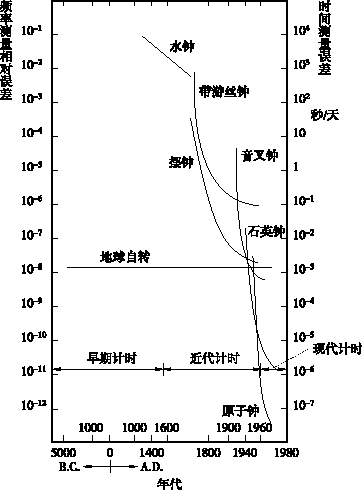
\includegraphics[height=8cm]{figure/fig01.01}
    \caption{不同年代的时间测量精度}
    \label{fig:01.01}
\end{figure}

图\ref{fig:01.01}~给出不同年代用不同的钟测量时间所达到的精度。可以
看到,地球自转要比各种机械的钟都好。所以,1967年以前是用
地球自转作为标准钟。原子钟是比地球自转更加稳定的钟,现代
的精密计时都是用原子钟了。

\begin{table}[!h]
    \centering
    \caption{一些典型物理现象的时间尺度}
    \label{tab:01.01}
    \begin{tabular*}{\linewidth}{>{\centering}m{\linewidth}c}
        \toprule
        \makecell[c]{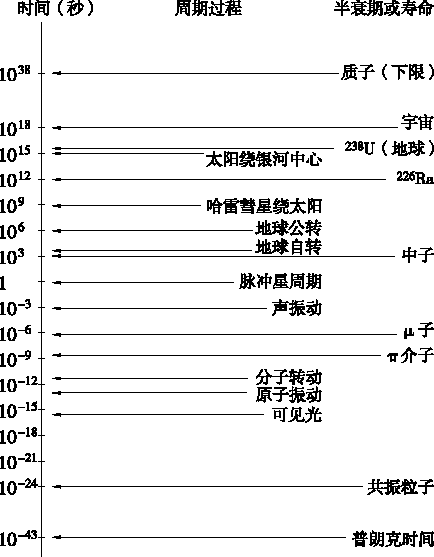
\includegraphics[width=0.8\linewidth]{figure/tab01.01}} & \\
        \bottomrule
    \end{tabular*}
\end{table}
\clearpage
1967年10月在第十三届国际度量衡会议上通过了新的标准
钟,它对一秒的时间作如下的规定;位于海平面上的$^{133}$Cs原子
的基态的两个超精细能级在零磁场中跃迁辐射的周期$T$与1秒的
关系为
\begin{equation*}
    1 \text{秒} = 9,192,631,770\,T
\end{equation*}

表\ref{tab:01.01}~列举了一些典型现象的时间尺度。目前,物理学中涉及
的最长的时间是:\num{e38}~秒,它是质子寿命的下限。宇宙的年龄大约
是~\num{6e17}~秒,即200亿年。牛顿力学所涉及的时问尺度大约是
\num{e-3}$\sim$\num{e15}~秒,即从声振动的周期到太阳绕银河中心转动的周期。
粒子物理的时间尺度都很小。$\mu$子的寿命是~\num{2e-6}~秒。已经算是
极长寿的了。最短寿的是一些共振粒子,它们的寿命只约有~\num{e-24}~
秒。目前物理学中涉及的最小的时间是~\num{e-42}~秒,称为普朗克时
间。普朗克时间被认为是最小的时间,比普朗克时间还要小的范
围内,时间的概念可能就不再适用了。
\section{芝诺佯谬和时间的度量}
\label{sec:01.02}
古希腊哲学家芝诺有一个很著名的论证:跑得最快的神话英
雄阿基里斯是永远追不上跑得最慢的东西(例如一只龟)的。他的
论证如下:因为开始时阿基里斯是在龟的后面,所以,阿基里斯
要追上龟,他必定先要到达龟的出发点,这要用有限的时间,在
这段时间里龟必定向前跑了,到达前面的一点,而当阿基里斯再
到达这点时,龟必定又已到达更前面的一点。如此重复下去,就
是进行无穷多次,龟也总不舍落在阿基里斯之后。

这个论证被称为芝诺佯谬,如何解开这个佯谬?

关键是在芝诺佯谬中用了两种不同的时间度量。按上节的讨
论,任何一种具有重复性的过程。都可以做为“钟”,用其重复
的次数来量度时间。芝诺问题中。除了“普通”钟所测得的时间
$t$,还利用了一种很特别的钟,该钟使用的重复性过程是。阿基里
斯逐次地到达龟在前一次的出发点。我们称这种钟叫芝诺钟,它
测得的时间为$t'$。

\begin{figure}[!h]
    \centering
    \vspace{-0.5em}
    \import{figure}{fig01.02.pdf_tex}
    \caption{芝诺时的定义}
    \label{fig:01.02}
    \vspace{-1.2em}
\end{figure}
如图\ref{fig:01.02},阿基里斯和龟在开始时相距为$L$,速度分别为$v_1$及
$v_2$,并且$v_1>v_2$。如果用普通的钟,则阿基里斯将在
\begin{equation}
    t=L/(v_1-v_2)
    \label{equ:01.02.01}
\end{equation}
时,赶上龟;当$t>L/(v_1-v_2)$时,阿基里斯就超过龟了。

图中左边的数字表示的是芝诺时$t'$。当$t'=1$时,阿基里斯到
达龟在0时的出发点;当$t'=2$时,阿基里斯到达龟在1时的出发
点。一般地,当$t'=n$时,阿基里斯到达龟在$t'=n-1$时的位置。
显然,只有当$t'\rightarrow\infty$时,阿基里斯才能逼近龟,对于任何有限的
$t'$,阿基里斯总是落在龟的后面。这就是芝诺的结论。

因此,芝诺断言:“阿基里斯永远也追不上龟。”这里“永
远”的含意是$t'\rightarrow\infty$。,即芝诺时间的无限。

现在我们来讨论普通时$t$与芝诺时$t'$之间的变换关系。不难
验证表\ref{tab:01.02}~给出的两种时间的对应。因此,一般有
\begin{equation}
    t=\sum_{n=0}^{t^{\prime}-1} \frac{L}{v_{1}}\left(\frac{v_{2}}{v_{1}}\right)^{n}=\frac{L}{v_{1}-v_{2}}\left[1-\left(\frac{v_{2}}{v_{1}}\right)^{t'}\right]
    \label{equ:01.02.02}
\end{equation}%
或者\vspace{-1.2em}
\begin{equation}
    t^{\prime}=\frac{1}{\ln \left(v_{2} / v_{1}\right)} \ln \left[1-\left(\frac{v_{1}-v_{2}}{L}\right) t\right]
    \label{equ:01.02.03}
\end{equation}%
式\eqref{equ:01.02.02}或式\eqref{equ:01.02.03}称为芝诺变换。它给出的$t'$与t的关系。在
图\ref{fig:01.03}~中画出。

\begin{table}[!h]
    \centering
    \vspace{-0.5em}
    \caption{普通时与芝诺时的关系}
    \label{tab:01.02}
    \begin{tabular}{c|l}
        \toprule
        芝诺时($t'$)& \hspace{7em}普通时($t$)\\
        \midrule
        0 & \qquad 0 \\
        \addlinespace
        1 & \qquad $\dfrac{L}{v_1}$  \\
        \addlinespace
        %\specialrule{0em}{3pt}{3pt}
        2 & \qquad $\dfrac{L}{v_1} + \dfrac{L}{v_1}\cdot\dfrac{v_2}{v_1}$ \\
        \addlinespace
        \vdots & \qquad \vdots \\
        \addlinespace
        $n$ & \qquad $\dfrac{L}{v_1} + \dfrac{L}{v_1}\cdot\dfrac{v_2}{v_1} + \dots + \dfrac{L}{v_1}\cdot(\dfrac{v_2}{v_1})^{n-1} $ \qquad \null\\
        \bottomrule
    \end{tabular}
    \vspace{-1.2em}
\end{table}
由图\ref{fig:01.03}~看到,芝诺变换是有奇性的,即当$t=L/(v_1-v_2)$时,
$t'\rightarrow\infty$。所以,当芝诺时$t'$从零变化到无限时,它只覆盖了普通时
$t$上的一个有限范围,即从零到$ L/(v_1-v_2) $。

因此,芝诺佯谬之“佯”,是由于芝诺把永远理解为$t'\rightarrow\infty$。
他认为$t'\rightarrow\infty$之后就没有时间了,故$t'\rightarrow\infty$相当于永远。实际上,
从图\ref{fig:01.03}~看到,在芝诺时$ t' $到达无限之后。还是有时间的。但是,
在该范围,即$ t>L/(v_1-v_2) $,用芝诺钟已经无法度量它们了。简
言之,芝诺的佯谬,来源于芝诺时的局限性,芝诺时不可能度量
阿基里斯追上龟之后的现象。

芝诺佯谬给我们的启示是,时间与时间的度量不同,一种时\clearpage
\begin{wrapfigure}[10]{10}{48mm}
%    \vspace{-0.5em}
    \import{figure}{fig01.03.pdf_tex}
    \caption{芝诺时的定义}
    \label{fig:01.03}
    %\vspace{-1.2em}
\end{wrapfigure}
\noindent 间的度量达到无限之后,还是可以有时间的;反之,一种时
间的度量达到无限,从其他的度量看,可能是有限的。

芝诺佯谬还启发我们提出一个更深入的问题,即所谓普通钟
或日常钟是否也具有芝诺钟那种局限性?当日常钟$t$的读数达到
无限之后,是否也还有时间?是否有$t$也无法度量的现象,即在
$t\rightarrow\infty$之外的现象?现代物理学的研究,对这些
问题的回答都是肯定的。

\section[长度]{长~~~~度}\label{sec:01.03}

长度是空间的一个基本性质。

对长度的测量,在日常的范围中,是用各种各样的尺,如米
尺、千分尺、螺旋测微计等等。对于不能用尺直接加以测量的小
尺度,可以求助于光学方法。在精密机床上常有光学测量装置;
测定胰岛索中原子的位置,是用X衍射方法。对于大的尺度,
也不能直接用尺去测量,也要求助于光。测量月亮与地球的距离
可以用激光测距的方法;测量一些不太远的恒星,可以用三角学
方法,利用恒星发出的光。至于银河系之外的遥远天体的距离,
同样是用它们发光的一些特征来测定的。

最近,长度的单位和标准,也用光来规定了。

长度的位单是米。1960年以前,用铂铱米尺作为标准尺,规
定米的大小。1960年以后,改用光的波长作为标准。在第十一届
国际计量大会上,正式通过的“米”的定义是l米等于$^{86}$Kr原子
的$2\rm{p}_{10}$和\erratanote{$5\rm{d}_5$}{原书作“$6\rm{d}_5$”,误。}~
能级之间跃迁时所对应的辐射在真空中的波长$\lambda$的l,650,763.73倍,即

\centerline{1米=l,650,763.73$\lambda$}

%\renewcommand{\hsp}{\hspace{0.6em}}

1983\ziju{0.05} 年10月召开的第十七届国际计量大会上已正式通过\ziju{0}
\\
\begin{tablex}[!h]{0.6em}
    \centering
    \caption{一些典型物理现象的空间尺度}
    \label{tab:01.03}
    \begin{tabular}{c}
        \toprule \vspace{-1em}                \\
        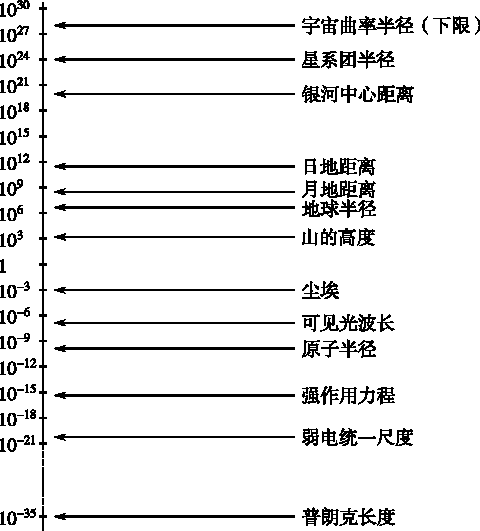
\includegraphics{figure/tab01.03} \\
        \bottomrule
    \end{tabular}
\end{tablex}
\clearpage

\noindent 了新的米的定义,即用光速值来定义“米”,以代替1960年的规定。
新的米的定义是,米是光在真空中在1,299,792,458秒的时间间隔
内所传播的路程长度。按这种新的定义,光速c是一固定的常数,即

\centerline{$c$=299,792,458米/秒}

表\ref{tab:01.03}~中列举了一些典型现象的空间尺度。目前,物理学中涉
及的最太长度是$10^{28}$米,它是宇宙曲率半径的下限;已达到的最
小长度为$10^{-20}$米,它是弱电统一的特征尺度。普朗克长度约为
$10^{-35}$米,被认为是最小的长度,意思是说,在比普朗克长度更小
的范围内,长度的概念可能就不再适用了。

\section[参考系]{参~~考~~系}\label{sec:01.04}

牛顿力学所研究的对象是物体的机械运动。从我们日常见到
的车行马跑,及至大到月亮、太阳等星体的运行,小到分子、原子、
粒子的一些飞行,都是属于这一类运动。这类运动的共同特点,
就是物体在空间的位置时刻在变化着。当然,静止的状态、平衡
的状态也是力学的内容之一。

牛顿意义下的运动学,就是研究如何描写物体位置的变化。

\renewcommand{\hsp}{\hspace{0.1em}}
研究问题总是从简单的情况入手。我们首先讨论一种被称为
质点的物体,即大小为零的物体。我们知道,任何具体的物体总
是有一定大小的,没有任何一个物体与质点完全等价。但是,对
于某些特定的运动来说,可以足够准确地把物体看作一个质点。
譬如,在讨论地球绕太阳的公转时,由于地球的半径\hsp(约\hsp 6,400\hsp 公
里)\hsp 比地球与太阳的距离\hsp (约\hsp 149,504,000\hsp 公里)\hsp 小得多,把地球作
为质点是相当好的近似,或者说,在此情况下,将地球作为质点
处理,是一个足够准确的模型。显然,这种模型是有一定适用限
度的。当讨论到地表问题时,再把地球看作质点就大谬不然了。

质点是一个物理对象。对于一个物理对象,用什么数学语言
来描写,这并不是一件很自然的事情,我们知道,任何一种数学
只是一种逻辑体系,一种逻辑体系能不能正确地描写我们的物理
对象,是要认真研究的。物理上,就是要寻找那种能正确地描写
物理对象的数学。在牛顿力学中,质点的空间几何性质,相当于
欧几里德几何上的点。在解析几何中,点的位置是由它的坐标值
来确定的。质点的位置也可以用这种坐标方法来给定。利用坐标
方法,首先要给出坐标系,坐标值总是相对于一定的坐标系而言
的。在数学上,坐标系的选取是完全任意的,但在物理上,我们
要对描写运动的各种物理量进行实际测量,坐标必须固定在一定
的物体上。例如,如果选取物体K上的某点O为坐标原点,并选
定$x$,$y$,$z$三个轴,质点$A$的位置即由$x$,$y$,$z$所确定(图1·4)。
这时,我们称所选取的物体$K$为参考系,而称坐标系$OXYZ$为参
考坐标系。

除了坐标方法外,也可以利用矢量方法来描写质点A的位
置。我们定义质点$A$的位置矢量$\vq{r}$的大小为$OA$的长度,而方向从
$O$指向$A$。用这个矢量就完全确定了质点$A$的位置。在图1.4的坐
标系中,位置矢量$r$的分量就是坐标$x$,$y$,$z$,或写为
\begin{align}\label{equ:01.04.01}
    \vq{r}=x\vq{i}+y\vq{j}+z\vq{k}
\end{align}
其中$\vq{i}$,$\vq{j}$,$\vq{k}$分别为$X$,$Y$,$Z$轴上的单位矢量,上述两种描述
质点$A$的位置的方法,是完全等价的。

参考系的选择是任意的,可以不用参考系$K$,而用另外一个
参考系$K'$,譬如,用运动着的车辆来描述质点$A$的位置。由图1·5
看到,对干参考系$K$,质点$A$的位置由矢量$\vq{r}$描写,而对于参考
系$K'$,由$\vq{r'}$描写。可见,对于同一个质点的位置,用不同参考系
来描写时,具有不同的位置矢量。就这一点,我们可以说,位
置是具有相对性的物理量。涉及物理量的相对性与绝对性的问题,
以后我们还要专门论述。
\section[轨迹]{轨~~~~迹}\label{sec:01.05}

谁都看到过,当喷气式飞机在飞行的时候,它的尾部泄出的
白烟在天空中构成形状美丽的各样曲线。这些曲线反映了飞机所
行经的路程。质点在运动中所经过的各点在空间连成一条曲线,
这条曲线我们称之为轨迹。

\begin{figure}[!h]
    \hspace{3em}
    \subfigure[\null]{
        \label{fig:01.06a}
        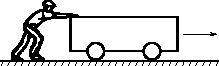
\includegraphics{figure/fig01.06a}
    }
    \hspace{3em}
    \subfigure[\null]{
        \label{fig:01.06b}
        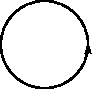
\includegraphics{figure/fig01.06b}
    }

    \hspace{3.7em}
    \subfigure[\null]{
        \label{fig:01.06c}
        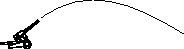
\includegraphics{figure/fig01.06c}
    }
    \hspace{1.3em}
    \subfigure[\null]{
        \label{fig:01.06d}
        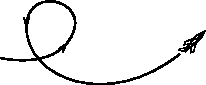
\includegraphics{figure/fig01.06d}
    }
    \caption{各种运动的轨迹}
    \label{fig:01.06}
\end{figure}

\clearpage

从图\ref{fig:01.06}~看到,各种运动的轨迹形状是不同的;\subref{fig:01.06a}图是直线,
\subref{fig:01.06b}图是圆周,\subref{fig:01.06c}图是抛物线,\subref{fig:01.06d}图是一般曲线。依照轨迹形状
的不同,可以把运动分为直线运动和曲线运动两大类。

如何描写轨迹呢?可利用曲线方程来描写。譬如,曲线方程 \begin{equation*}
    \begin{aligned}
        &x^2+y^2=r^2 \\[-0.5em]
        &z=0
   \end{aligned}
\end{equation*}
就描写了在$z=0$平面上半径为$r$的圆周运动的轨迹。一般曲线方
程可以表示成
\begin{equation*}
    \begin{aligned}
        f_1\left(x,y,z\right)=0 \\[-0.5em]
        f_2\left(x,y,z\right)=0
    \end{aligned}
\end{equation*}

在历史上很长一个时期内,人们只注重轨迹形状的研究,例
如行星走圆形,落体走直线。我们知道,质点运动是位置的变化,
它涉及空间和时间两方面。轨迹形状只反映了运动的空间方面的
性质,它对于研究运动还是不够的,因为轨迹还没有把质点运动
的情况全部表述出来,特别是没有表述它的动态性质。百米赛跑
时,所有运动员的轨迹都是直线,但他们各自的运动情况并不全
同,否则就分不出名次了。我们不仅应该知道轨迹,而且还应知
道质点经过轨迹上各点的时刻。运动是在时间、空间里的现象,
关键是把时间描写和空间描写联系起来。直到牛顿之前不久,才
特别强调了这一点。

下面,我们举两个直线运动的例子。

对于在平直铁轨上稳定运动的列车上的某一点,所测得的各
时刻的位置列于表\ref{tab:01.04}~中,其中位置坐标$x$是以铁轨为参考系的(图\ref{fig:01.07})。
\vspace{-1em}
\begin{tablex}[!h]
    \caption{}
    \label{tab:01.04}
    \centering
        \begin{tabularx}{\linewidth}{c*{6}{|C}}
            \toprule
            时~~~~间(秒) & 0 & 1  & 2  & 3  & 4  & 5  \\
            \midrule
            位置坐标(米) & 0 & 17 & 34 & 51 & 68 & 85 \\
            \bottomrule
        \end{tabularx}
\end{tablex}

\begin{figurex}[!h]
    \centering
    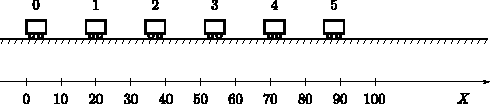
\includegraphics{figure/fig01.07}
    \caption{列车的运动}
    \label{fig:01.07}
\end{figurex}

对于从地面上某一高度自由落下的质点(称为自由落体),轨
迹也是一条直线。如果我们取如图\ref{fig:01.08}~所示的坐标系,则所测得的
质点在各时刻的位置列在表\ref{tab:01.05}~中。
\begin{tablex}[!h]
    \caption{}
    \label{tab:01.05}
    \centering
        \begin{tabularx}{\linewidth}{c*{5}{|C}}
            \toprule
            时~~~~间(秒) & 0 & 1   & 2    & 3    & 4    \\
            \midrule
            位置坐标(米) & 0 & 4.9 & 19.6 & 44.1 & 78.4 \\
            \bottomrule
        \end{tabularx}
\end{tablex}

用数学的语言说,表\ref{tab:01.04}~和表\ref{tab:01.05}~是给出了质点的位置坐标与
时间之间的函数关系,这个函数关系$x\left(t\right)$,称之为轨迹函数,或
\begin{wrapfigure}[14]{l}{8em}
    \centering
    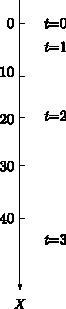
\includegraphics{figure/fig01.08}
    \\ ~ \\
    \caption{落体的运动}
    \label{fig:01.08}
\end{wrapfigure}
运动方程式、运动解。

为了便于进行计算,我们常希望能把轨迹
函数$x\left(t\right)$写成简单的分析表达式。对于表\ref{tab:01.04}~
的$x\left(t\right)$,可以写成
\begin{equation}\label{eqn:01.05.01}
    x=17t
\end{equation}
对于表\ref{tab:01.05}~的运动,可以写成$x=4.9t^2$。

对于曲线运动,轨迹函数就是位置矢量$\vec{r}$作为时间
$t$的函数,亦即$\vec{r}\left(t\right)$。随着$t$的变化,位置矢量$\vec{r}$的
端点在空间所划出的曲线,就是质点运动的轨迹(图\ref{fig:01.09})。也可
以用质点的三个坐标的函数$x\left(t\right)$,$y\left(t\right)$及$z\left(t\right)$来描写运
动,它们与$r\left(t\right)$的关系是
\clearpage
\begin{equation}\label{eqn:01.05.02}
    \vec{r}\left(t\right)=x\left(t\right)\vec{i}+y\left(t\right)\vec{j}+z\left(t\right)\vec{k}
\end{equation}

\begin{wrapfigure}[7]{r}{11em}
    \centering
    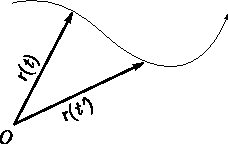
\includegraphics{figure/fig01.09}
    \caption{曲线运动}
    \label{fig:01.09}
\end{wrapfigure}
轨迹也具有相对性。譬如对于从地面上某一高度自由下落的质点,以
地面为参考系,看到轨迹是一条直线;而相对于沿平直铁轨稳定运行的
列车来说,轨迹则是一条抛物线。同一个物体的运动,在不同的参考系中
看到的轨迹形状不一定相同。

另一方面,对于时间,也必须选取一定的标准,即选取时间
原点,才能进行测量。而时间原点的选取,也有任意性,不同的
选取法,使轨迹函数的形式也有些差别。

因此,参考系的概念要作些扩充。选取一个参考系应包括:
给定放置在某物体上的坐标系,作为测量空间的标准;以及给定
一个钟,作为测量时间的标准。
\section{速度的瞬时性}
\label{sec:01.06}
    机械运动的现象,给了我们对“快”、“慢”的经验认识。
火车比轮船快,飞机比火车快,而火箭更比飞机快等等。反映质
点运动快慢的物理量就是速度,或者确切地说,是速度的数值大
小。
    先以直线运动为例,当时刻t1时,质点A的位置坐标为x(t1),
当t2时,它的坐标为x(t2),我们就用下式来定义质点A在t1到
t2时间间隔内的平均速度:
\begin{equation}
    \langle v\rangle_{t_{1} \rightarrow t_{2}}=\frac{x(t_{2})-x(t_{1})}{t_{2}-t_{1}} \label{equ:01.06.01}
\end{equation}
符号$\langle \rangle$表示所讨论的量的平均值。$\langle v\rangle_{t_{1} \rightarrow t_{2}}$的数值表示质点
在时间间隔$t_{1} \rightarrow t_{2}$中每单位时同平均走过的距离,它的单位是
米/秒。利用表\ref{tab:01.04}所给出的运动进行计算,就有:在第1秒末到
第2秒末间隔中,
\begin{equation*}
    \langle v\rangle_{1 \rightarrow 2}=\frac{34-17}{2-1}=17\text{米/秒}
\end{equation*}
在第3秒末到第5秒末间隔中,
\begin{equation*}
    \langle v\rangle_{3 \rightarrow 5}=\frac{85-51}{5-3}=17\text{米/秒}
\end{equation*}
选两个时间间隔中平均速度是一样的。事实上,如果利用分析表
达式\ref{equ:01.05.01}~来计算,就会发现对任何时间间隔,运动的平均速度
都是17米/秒。这种对于任何时间间隔平均速度总不变的运动,称
为匀速直线运动.
    由表\ref{tab:01.05}~或$x=4.9t^2$所示的自由落体运动,情况就不同了:
在第1秒末到第3秒束的问隔中,
\begin{equation*}
    \langle v\rangle_{1 \rightarrow 3}=\frac{44.1-4.9}{3-1}=19.6\text{米/秒}
\end{equation*}
在第1秒末到第2秒末的间隔中,
\begin{equation*}
    \langle v\rangle_{1 \rightarrow 2}=\frac{19.6-4.9}{2-1}=14.7\text{米/秒}
\end{equation*}
在第2秒末到第3秒末的间隔中,
\begin{equation*}
    \langle v\rangle_{2 \rightarrow 3}=\frac{44.1-19.6}{3-2}=25.4\text{米/秒}
\end{equation*}
对于不同的时间间隔。自由落体的平均速度不相同。这种运动称
为变速运动。从上面所给出的三个平均速度可知,自由落体在第
1秒末到第3秒末的两秒钟时间间隔中并非匀速,它在前一秒钟
(即第1秒末到第2秒末)平均速度较小,在后一秒钟(即第2秒末
到第3秒末)平均速度较大。从这一点上可以充分反映出平均速度
往往不足以描写变速运动的细致情况。这是平均速度概念的弱
点。求平均速度的时间间隔取得越大,它对快慢的描述就越粗略;
反之,时间间隔越小,对快慢的描述也就越精确。在上例中,虽
然取1秒的时间间隔,比取2秒的时间间隔要好一些,但是在一
秒钟的时间间隔内,自由落体仍然不是匀速的。这种情况迫使我
们把计算平均速度的时间间隔取得尽可能地小。

    为了便于进一步讨论,我们将式\ref{equ:01.06.01}~中的
$t_2$表示成$t_2=t_1+\Delta t$,这个$\Delta t$就是求平均速
度所选用的时间间隔。现在来求从第1秒末到第$1+\Delta t$秒末
的间隔中,自由落体的平均速度。利用$x=4.9t^2$得到
\begin{equation*}
    \begin{aligned}
        \langle v\rangle_{1 \rightarrow 1+\Delta t} &=\frac{x(1+\Delta t)-x(1)}{1+\Delta t-1} \\
        &=\frac{4.9 \times(1+\Delta t)^{2}-4.9 \times 1^{2}}{\Delta t} \\
        &=(9.8+4.9 \Delta t) \text { 米/秒 }
    \end{aligned}
\end{equation*}
此式再次表明,从第1秒末开始取不同的时间间隔$\Delta t$,所得的平
均速度是不相同的。既然$\Delta t$越小描述得越精确,我们取
$\Delta t$为无限小,或者相当于$\Delta t \rightarrow 0$的
极限情况,这时平均速度变成为:
\begin{equation*}
    \lim _{\Delta \rightarrow 0}(9.8+4.9 \Delta t)=9.8 \text { 米/秒 }
\end{equation*}
这个9.8米/秒的物理意义是自由落体在第1秒末的一个无限小时
间间隔中的平均速度,我们称这个值为自由落体在第1秒末的瞬
时速度。瞬时速度与平均速度这两个概念的重要区别在于:平均
速度总是与一段有限的时间间隔相联系,它是描述一段运动过程
的物理量;相反,瞬时速度与一个时刻相联系,它是描述运动的
瞬时性质的物理量。有了瞬时速度这个概念,使我们对运动的认
识大为深化。
    用类似的手续不难求出自由落体运动在任何时刻t的瞬时速
度$v(t)$,只要将上述的1及$1+\Delta t$分别代之以$t$及$t+\Delta t$,并取
于$\Delta t \rightarrow 0$的极限值就可以了。故有
\begin{equation}
    \begin{aligned}
        v(t) &=\lim _{\Delta t \rightarrow 0} \frac{x(t+\Delta t)-x(t)}{\Delta t} \\
        &=\lim _{\Delta t \rightarrow 0} \frac{4.9 \times(t+\Delta t)^{2}-4.9 \times t^{2}}{\Delta t} \\
        &=\lim _{\Delta t \rightarrow 0}(9.8 t+4.9 \Delta t) \\
        &=9.8 t \label{equ:01.06.02}
    \end{aligned}
\end{equation}
此式给出了自由落体在每个时刻的瞬时速度。根据这个结果,我
们再强调一遍,自由落体的运动快慢是时刻变化着的。你用平均
速度来描写它,无论$\Delta t$取如何小的有限值,即使小到$\Delta t$=0.001
秒,依然不够精确,因为在这0.001秒中质点依然不是匀速运动
的。只有$\Delta t$趋于无限小,给出了每个时刻$t$的瞬时速度,了解了
质点运动在每一瞬时的快慢,才算最精确地反映了质点运动的快
慢。
    对于任何直线运动,它的瞬时速度都可以用类似方式来确
定:
$$
v(t)=\lim _{\Delta \rightarrow 0} \frac{x(t+\Delta t)-x(t)}{\Delta t}
$$
根据微积分学的知识,该极限就是轨迹函数x(t)对时间t的一阶
导数。即
\begin{equation}
    \begin{aligned}
        v(t) &=\lim _{\Delta t \rightarrow 0} \frac{x(t+\Delta t)-x(t)}{\Delta t} \\
        &=\lim _{\Delta t \rightarrow 0} \frac{\Delta x}{\Delta t}=\frac{d x}{d t} \label{equ:01.06.03}
    \end{aligned}
\end{equation}
其中,$\Delta x=x(t+\Delta t)-x(t)$,是在$t\rightarrow t+\Delta t$时间间隔中质点位置
坐标的增量。以后我们提到的速度,一般都指瞬时速度。

    我们看到,瞬时速度是利用数学上的微分概念来描写的。其
实,在历史上,正是由于牛顿在处理这类基本力学问题时需要一
种适当的数学工具,从而促使他创建了微积分学。这不仅使物理
概念得以准确地表述,而且也大大丰富了数学本身。这是牛顿的
巨大功绩之一。由此,我们再次看到,一个物理对象,用什么数学
语言描写并不是一件自然的事情,而是物理研究的一个核心课题。
    当质点作直线运动时,我们
可以设法求出它的位置时间曲线
(图l.10)。从图中可以看出,平
均速度在数值上等于各段割线的
斜率,瞬时速度在数值上等于各
点的切线的斜率。所以在求出位
置时间曲线后,就可以从$x(t)$曲
线上求出各点的速度。
  从平均速度的定义(\ref{equ:01.06.01})式可以知道,$\langle v\rangle$可以有正值,
也可以有负值。当$x(t+\Delta t)<x(t)$时,$\langle v\rangle$为负。这种情况相当
于质点在$t$到$t+\Delta t$间隔中,总的说来是向负$x$方向运动的。所
以,$\langle v\rangle$的正负恰恰反映了运动的方向。通常称平均速度的绝对
值$|\langle v\rangle|$为平均速率。类似地,瞬时速度的绝对值$|v(t)|$被称为
速率,而瞬时速度的正负,就表示质点在时刻$t$的运动方向。速
度$v$不仅描述了运动的快慢,而且描述了运动方向。
\section{曲线运动的速度}\label{sec:01.07}

\ziju{-0.02}我们现在来推广上节关于直线运动的速度的概念。按图1.11,
质点作曲线运动,在时刻$t_1$,质点位置矢量为$\vec{r}\left(t_1\right)$,在时刻$t_2$,
位置矢量为$\vec{r}\left(t_2\right)$,则定义在$t_1$到$t_1$间隔中质点A的平均速度为\ziju{0}
\begin{equation}\label{eqn:01.07.01}
    \langle v \rangle_{t_1\rightarrow t_2}=\frac{\vec{r}\left(t_2\right)-\vec{r}\left(t_1\right)}{t_2-t_1}=\frac{\Delta \vec{r}}{\Delta t}
\end{equation}

\noindent 将其与式\eqref{eqn:01.06.01}~对比可见。只是将其中的$x\left(t\right)$换成了相应的
$\vec{r}\left(t\right)$。在\eqref{eqn:01.07.01}~中,$\Delta t=t_2-t_1$,$\Delta \vec{r}=\vec{r}\left(t_2\right)-\vec{r}\left(t_1\right)$,
后者是$t_1$到$t_2$间隔
\begin{wrapfigure}[8]{r}{12em}
    \centering
    \small
    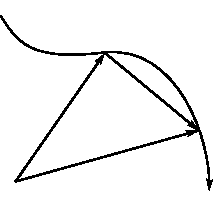
\includegraphics{figure/fig01.11}
    \caption{曲线运动的速度}
    \label{fig:01.11}
\end{wrapfigure}
中质点位置矢量的改变量,称为位移矢量。这个平均速度的定义表明,平均速度是矢量。根据矢量运算
规则,式\eqref{eqn:01.07.01}~所定义的$\langle v\rangle t_1-t_2$是在l到2的方向(图\ref{fig:01.11})。
另一方面,由图\ref{fig:01.11}~很清楚知道,在$t_1$到$t_2$时间内质点$A$的运
动方向并非总是沿着l到2的方向的,而是先从1向3方向运动,
然后从3向2方向运动,这些运动方向并不平行于1到2的方向。
所以平均速度所指的方向,只是质点$A$真实运动方向的平均。
也就是说,平均速度不但对于运动快慢的描写是粗
略的,而且对于运动方向的描写也是粗略的。

对式\eqref{eqn:01.07.01}~取$\Delta t \rightarrow 0$的极限,就得到瞬
时速度的定义。
\begin{equation}\label{eqn:01.07.02}
    \begin{aligned}
        \vec{v}\left(t\right) & =\lim _{\Delta t \rightarrow 0} \frac{\vec{r}\left(t+\Delta t\right)-\vec{r}\left(t\right)}{\Delta t} \\
                  & =\lim _{\Delta t \rightarrow 0} \frac{\Delta \vec{r}}{\Delta t} =\frac{\dif\vec{r}}{\dif t}
    \end{aligned}
\end{equation}
它是直线运动情况的式\eqref{eqn:01.06.03}的推广。如果利用式\eqref{eqn:01.04.01},则
有
\begin{equation}\label{eqn:01.07.03}
    \vec{v}\left(t\right)=\frac{\dif x\left(t\right)}{\dif t} \vec{i}+\frac{\dif y\left(t\right)}{\dif t} \vec{j}+\frac{\dif z\left(t\right)}{\dif t} \vec{k}
\end{equation}
所以三个坐标函数$x\left(t\right)$,$y\left(t\right)$,$z\left(t\right)$对时间t的导数分别是速度矢
量在三个坐标轴方向的分量:
\begin{equation}\label{eqn:01.07.04}
    v_{x}=\frac{\dif x\left(t\right)}{\dif t}, ~ v_{y}=\frac{\dif y\left(t\right)}{\dif t}, ~ v_{z}=\frac{\dif z\left(t\right)}{\dif t}
\end{equation}
\clearpage
\begin{wrapfigure}[7]{r}{13em}
    \centering
    \small
    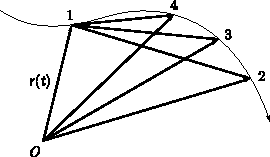
\includegraphics{figure/fig01.12}
    \caption{曲线运动的瞬时速度}
    \label{fig:01.12}
\end{wrapfigure}
由图\ref{fig:01.12},当$\Delta t$减小时,矢量$\vec{r}\left(t+\Delta t\right)$
逐渐向$\vec{r}\left(t\right)$靠拢,矢量$\Delta \vec{r}$相继从1,2变到1,3,
变到1,4……,在$\Delta t \rightarrow 0$的极限情况下,$\Delta \vec{r}$
的方向趋于轨迹曲线在点1的切线方向。这样,我们就得到一个
结论:瞬时速度$\vec{v}\left(t\right)$的方
向,就是轨迹曲线在相应点的切线方向。瞬时速度的大小$v$,按
定义\eqref{eqn:01.07.02}应为
\setlength{\mathindent}{15em}
\begin{equation*}
    \begin{aligned}
        v\equiv |\vec{v}| & =\left|\lim _{\Delta t \rightarrow 0} \frac{\Delta \vec{r}\left(t\right)}{\Delta t}\right| \\
                         & =\lim _{\Delta t \rightarrow 0} \frac{|\Delta \vec{r}|}{\Delta t}
    \end{aligned}
\end{equation*}

\setlength{\mathindent}{6em}
\begin{wrapfigure}[4]{l}{10em}
    \vspace{-6em}
    \centering
    \small
    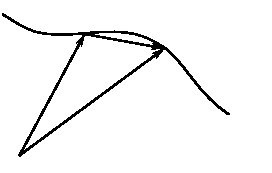
\includegraphics{figure/fig01.13}
    \caption{用路程长度$s\left(t\right)$来描写运动}
    \label{fig:01.13}
\end{wrapfigure}
\noindent 我们可以引入路程长度概念来描写运动。如图\ref{fig:01.13},若当$t=0$时,
质点在轨迹上的$P$处。则可定义函数$s\left(t\right)$,它表示质点到$t$时刻所
走过的路程的长度。显然,$\Delta s=s\left(t+\Delta t\right)-s\left(t\right)$表示
在$t$到$t+\Delta t$中质点所走过的路程的长度。一般$\Delta s$和
$|\Delta \vec{r}|$并不相等,但在$\Delta t \rightarrow 0$的极限情况
下,二者是一样的,故速度大小也可表示为
\begin{equation}\label{eqn:01.07.05}
    v=\lim_{\Delta t \rightarrow 0}\frac{\Delta s}{\Delta t}=\frac{\dif s}{\dif t}
\end{equation}


\section{加速度}\label{sec:01.08}

为了描写速度的变化,我们再引入一个物理量,即所谓加速
度。对于直线运动,若当$t$时刻,质点速度为$v(t)$,$当t+\Delta t$时
刻,为$v(t+\Delta t)$,则我们定义从$t$到$t+\Delta t$间隔中质点的平均加
速度为
\vspace{-1em}\begin{equation}\label{eqn:01.08.01}
    \langle a\rangle_{t\rightarrow t+\Delta t} = \frac{v(t+\Delta t)-v(t)}{\Delta t}
\end{equation}
它的定义是质点在单位时间中速度的平均变化,单位是$\text{米/秒}^2$。

利用式\eqref{eqn:01.06.02},可以计算自由落体在$t$到$t+\Delta t$间隔中的平
均加速度:
\vspace{-0.5em}\begin{equation*}
    \begin{aligned}
        \langle a\rangle_{t\rightarrow t+\Delta t} & = \frac{9.8(t+\Delta t)-9.8t}{\Delta t} \\
                                                   & = 9.8\text{米/秒}^2
    \end{aligned}
\end{equation*}
这个结果中不含$t$和$\Delta t$,也就是说,对任何一段时间间隔,自由落
体的平均加速度都是一样的。这种加速度不随时间变化的运动,
称为匀加速运动。自由落体运动是一个典型的匀加速运动。无论
用何种材料作成的物体,它的自由落体加速度总等于9.8~$\text{米/秒}^2$。
称此加速度为重力加速度,用$g$表示。

精确测量表明,在地球各处,重力加速度$g$并不都一样,一
\begin{tablex}[!h]
    \vspace{-1em}
    \caption{地球上不同地点的$g$值}
    \label{tab:01.06}
    \centering
        \setlength{\tabcolsep}{1.5em}
        \begin{tabularx}{\linewidth}{l|l|S}
            \toprule
            地~~点             & 纬~~~度      & $g$(米/秒) \\
            \midrule
            北~~极             & 北纬\ang{90} & 9.83245      \\
            戈拉雅克(格陵兰)   & 北纬\ang{70} & 9.8253       \\
            雷克雅未克(冰岛)   & 北纬\ang{64} & 9.8227       \\
            列宁格勒           & 北纬\ang{60} & 9.8193       \\
            巴~~黎             & 北纬\ang{49} & 9.8094       \\
            北~~京             & 北纬\ang{40} & 9.8012       \\
            汉~~口             & 北纬\ang{30} & 9.7936       \\
            广~~州             & 北纬\ang{23} & 9.7883       \\
            蒙罗维亚(利比里亚) & 北纬\ang{6}  & 9.7816       \\
            雅加达             & 南纬\ang{6}  & 9.7813       \\
            墨尔本             & 南纬\ang{38} & 9.7999       \\
            \bottomrule
        \end{tabularx}
\end{tablex}
\clearpage
\noindent 般说来,在低纬度处$g$值较小;在高纬度处,$g$值较大(表\ref{tab:01.06})。

类似于平均速度不足以细致地描写非匀速运动一样,平均加
速度也不足以细致地描写非匀加速运动。对于非匀加速运动,必
须引入瞬时加速度来描述它的速度变化。加速度也是一个描述运
动的瞬时性质的物理量。瞬时加速度定义为:
\begin{equation*}
    \begin{aligned}
        a(t) & =\lim _{\Delta t \rightarrow 0} \frac{v(t+\Delta t)-v(t)}{\Delta t} \\
             & =\frac{\dif v(t)}{\dif t}=\frac{\dif^2 x(t)}{\dif t^2}
    \end{aligned}
\end{equation*}
它的意义是质点在时刻t的无限小时间间隔中的平均加速度。以
后我们谈到加速度,一般都是指瞬时加速度。

对于一般的曲线运动,可以给出相应的平均加速度及瞬时加
速度为:
\begin{equation}\label{eqn:01.08.02}
    \langle \vec{a} \rangle_{t \rightarrow t+\Delta t} = \frac{\vec{v}(t+\Delta t)-\vec{v}(t)}{\Delta t}
\end{equation}
\begin{equation}\label{eqn:01.08.03}
    \begin{aligned}
        \vec{a}(t) & =\lim _{\Delta t \rightarrow 0} \frac{\vec{v}(t+\Delta t)-\vec{v}(t)}{\Delta t} \\
                  & =\lim_{\Delta t \rightarrow 0}\frac{\Delta \vec{v}}{\Delta t}                  \\
                  & =\frac{\dif\vec{v}(t)}{\dif t}=\frac{\dif^2 \vec{r}(t)}{\dif t^2}
    \end{aligned}
\end{equation}
在曲线运动情况下,速度方向是变化的。$v(t)$,$v(t+\Delta t)$及$\Delta v$,
\begin{wrapfigure}[6]{r}{13em}
    %\vspace{-6em}
    \centering
    \small
    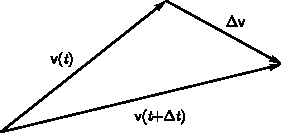
\includegraphics{figure/fig01.14}
    \caption{加速度的计算}
    \label{fig:01.14}
\end{wrapfigure}
一般如图\ref{fig:01.14}~所示。由于$a$平行于$\Delta v$,所以平均加速度的方向一
般与速度方向并不相同。瞬时加速度也类似。当加速度方向平行
于速度时,表示速度方向没有变化,但速率增加。当二者反平行
时,表示速度方向不变,而速率减少。当加速度既不平行也不反
平行于速度时,表示速度方向也在变化。

利用式\eqref{eqn:01.07.03},加速度矢量的分量可以表示为:
\begin{equation}\label{eqn:01.08.04}
    \vec{a}=\frac{\dif^2x(t)}{\dif t^2}\vec{i}+\frac{\dif^2y(t)}{\dif t^2}\vec{j}+\frac{\dif^2z(t)}{\dif t^2}\vec{k}
\end{equation}
加速度的三个坐标分量为:
\begin{equation}\label{eqn:01.08.05}
    a_x=\frac{\dif^2x(t)}{\dif t^2},~ a_y=\frac{\dif^2y(t)}{\dif t^2},~
    a_z=\frac{\dif^2z(t)}{\dif t^2}
\end{equation}
$\vec{r}$,$\vec{v}$,$\vec{a}$是描写运动的物理量。我们希望用数目比较少的物
理量来描写运动。什么叫比较少?意思是这些物理量之间应是相
互独立的。所谓相互独立。是说其中任一个量不能由其他的量加
以确定。用$\vec{r}$,$\vec{v}$及$\vec{a}$三个量来描写运动是必要的,因为它们是相互
独立的。例如,在某一时刻,知道了质点的位置$\vec{r}$,并不能知道
它的速度$\vec{v}$,知道了$\vec{v}$,也并不能知道$\vec{a}$,反之亦然。人们认识到
这一点,也并不容易。在伽利略之前,并没有加速度概念。当时,
没有人认识到加速度与速度是相互独立的,所以没有认识到需要
用加速度来描写运动。

我们已讨论了位置矢量、速度和加建度。从运动学本身来考
虑,没有足够的理由说明,为什么我们应当到此为止,而不去讨
论加加速度、加加加速度……。当然,我们可以定义并计算加加
速度,即加速度的变化率,但一般说这并不代表任何具有基本物
理价值的东西。其中的原因在动力学,学过动力学后,我们将看
到,对力学的讨论几乎全部是基于位置矢量,速度和加速度这三
个量。

下面我们介绍运动的独立性这一重要概念。由式\eqref{eqn:01.05.02}、
\eqref{eqn:01.07.03}、\eqref{eqn:01.08.05}可以看到,描写一个复杂的曲线运动时,$X$方
向的坐标、速度、加速度与其他方向的坐标,速度、加速度无关。
$Y$方向和$Z$方向也有这种性质,即三个方向相互无关,这种性质被
称为运动的独立性。因此,一个复杂的曲线运动,可看成在$X$,$Y$,
$Z$三个方向上的直线运动,这三个运动同时进行,我们可以对每
一个运动进行单独的分析,好象另外两个自由度上的运动是根本
不存在一样,这样就使问题变得简单。

\example 已知一个质点作直线运动。观察到它的位置与时间
的变化如表\ref{tab:01.07}所示。用这些数据求出各时间间隔的平均速度$v$及
平均加速度$a$,并写出运动方程式。
\begin{tablex}[!h]
    \caption{}
    \label{tab:01.07}
    \centering
    \begin{tabularx}{\linewidth}{l*{9}{|C}}
        \toprule
        时~~~~间(秒) & 0 & 1 & 2 & 3 & 4 & 5 & 6 & 7 & 8 \\
        \midrule
        \makecell{与参考点的距离                           \\(米)}  &  3  &  4  &  9  &  18  &  31  &  48  &  69  &  94 & 123 \\
        \bottomrule
    \end{tabularx}
\end{tablex}

\solution 因为时间间隔都是1秒,即$\Delta t=1$秒。所以从数值上有
\begin{align*}
    v & =\frac{\Delta s}{\Delta t}=\Delta s                         \\
    a & =\frac{(v_2-v_1)}{\Delta t}=v_2-v_1=(\Delta s_2)-(\Delta s_1)
\end{align*}
将结果列于表\ref{tab:01.08}中。
\begin{tablex}[!h]
        \caption{}
        \label{tab:01.08}
        \centering \zihao{-5}
        \setlength{\tabcolsep}{0em}
        \begin{tabularx}{\linewidth}{l*{17}{|C}}
            \toprule
            时~~~~间(秒)                              & 0 &   & 1 &   & 2 &   & 3  &    & 4  &    & 5  &    & 6  &    & 7  &    & 8   \\
            \midrule
            与参考点的距离(米)                        & 3 &   & 4 &   & 9 &   & 18 &    & 31 &    & 48 &    & 69 &    & 94 &    & 123 \\
            各秒内的位置变化($\Delta s$)(米)          &   & 1 &   & 5 &   & 9 &    & 13 &    & 17 &    & 21 &    & 25 &    & 29 &     \\
            各秒内的平均速度($v$)(米/秒)              &   & 1 &   & 5 &   & 9 &    & 13 &    & 17 &    & 21 &    & 25 &    & 29 &     \\
            各秒内的平均加速度($a$)($\text{米/秒}^2$) &   &   & 4 &   & 4 &   & 4  &    & 4  &    & 4  &    & 4  &    & 4  &    &     \\
            \bottomrule
        \end{tabularx}
\end{tablex}
\clearpage
既然平均加速度$a$是一个常数,所以这个直线运动是匀加速
直线运动,加速度是$a=4$米/秒$^2$.对于匀加速直线运动,一般的
运动方程是:
%\vspace{-1em}
\begin{equation*}
    s=s_0+v_{0}t+\frac{1}{2}at^2 \vspace{-0.5em}
\end{equation*}
用已知数据代入,便可求出$s_0$,$v_0$,$a$。

当$t=0$时,$s=s_0=3$,所以$s_0=3$;

当$t=1$时,$4=3+v_0+\dfrac 1 2 a$,即$v_0+\dfrac 1 2 a=1$;

当$t=2$时,$9=3+2v_0+2a$,即$v_0+a=3$。

解上述两方程可得$a=4$,$v_0=-1$。所以运动方程式为:
\begin{equation*}
    s=3-t+2t^2
\end{equation*}

\example 在阴极射线管中,一束电子以$10^9$厘米/秒的速度水
平地射入平行板之间的均匀电场,电场使电子获得$10^{17}$厘米/秒$^2$
的向下的匀加速度。己知平行板长为2厘米。求:

\begin{wrapfigure}[8]{r}{16em}
    \centering
    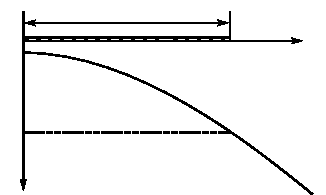
\includegraphics{figure/fig01.15}
    \caption{}
    \label{fig:01.15}
\end{wrapfigure}
(1)电子束通过平行板时的竖直方向位移$d$和经历
的时间$t$;

(2)电子束离开平行板时的速度大小和方向;

(3)在平行板内和离开板后电子束的轨迹。

\solution 选择如图\ref{fig:01.15}~所示的坐标系。

由于运动的独立性,在$x$方向是惯性运动,速度为$v_0=10^9$厘
米/秒;在$y$方向是匀加速运动,加速度为$a=10^{17}\text{厘米/秒}^2$(因为$a$
远远大于重力加速度$g$,所以不考虑重力的影响),且初速为零,
故有:

~\vspace{-1em}
\begin{equation*}
    \left\lbrace \begin{aligned}
        x & =v_0 t               \\
        y & =\frac{1}{2}at^2+y_0
    \end{aligned}\right.
\end{equation*}
电子通过平行板的时间为:
\begin{equation*}
    t_0=\frac{l}{v_0}=\frac{2}{10^{9}}=\num{2e-9}\text{秒}
\end{equation*}
电子通过平行板时,在竖直方向的位移为:
\begin{align*}
    d & =y_1-y_0                                     \\
      & =\frac{1}{2}at_0^2                           \\
      & =\frac{1}{2}\times 10^{17} \times \num{4e-18} \\
      & =0.2\text{厘米}
\end{align*}
电子在板中时,因为\vspace{-0.5em}
\begin{equation*}
    v_x=v_0 \qquad v_y=at \\
\end{equation*}
所以\vspace{-1em}
\begin{equation*}
    v=\sqrt{v_x^2+v_y^2}=\sqrt{v_0^2 + a^2 t^2}
\end{equation*}
速度与水平轴的夹角为:
\begin{equation*}
    \theta = \arctg\frac{v_y}{v_x} = \arctg\frac{at}{v_0}
\end{equation*}
它随时间而变。在离开板时,$t=t_0$,有
\begin{align*}
     & v \approx \num{1.02e9}\text{厘米/秒}                           \\
     & \theta = \arctg\frac{at_0}{v_0} =\arctg\frac 1 5=\ang{11;19;}
\end{align*}
在板内运动方程是:
\begin{equation*}
    \left\lbrace \begin{aligned}
        x & =v_0 t               \\
        y & =\frac{1}{2}at^2+y_0
    \end{aligned}\right.
\end{equation*}
消去$t$则得$y=\dfrac{a}{2v_0^2}x^2+y_0$,轨迹是抛物线。

离开平行板后。电子以与水平轴成\ang{11;19;}的夹角的速度
$v\approx\num{1.02e8}$厘米/秒作直线运动。

\example 设在地面附近,重力加速度是个常数$g$,且垂直指向
地面。物体的初速度为$ v_0 $。与水平方向成$ \theta $角。试讨论抛体运动
轨迹。

\discussion 我们在$ v $和铅垂线所决定的平面上来研究。按图\ref{fig:01.16}~
中的坐标,可把运动分解为$ x $方向与$ y $方向,并分别处理。$ x $方向
是惯性运动$ v_x=v_0\cos\theta $,所以有
\begin{equation*}\label{xeqn:01.08.01}
    x=(v_0\cos\theta)t \tag{1}
\end{equation*}
$ y $方向就是上抛运动,初速度为$ v_0\sin\theta$。故有
\begin{align*}
\label{xeqn:01.08.02} &v_y=v_0\sin\theta-gt \tag{2} \\
\label{xeqn:01.08.03} &y=(v_0\sin\theta)t-\frac{1}{2}gt^2 \tag{3}
\end{align*}
由\eqref{xeqn:01.08.01},\eqref{xeqn:01.08.03}消去$ t $便得抛物线形的轨迹:
\begin{equation*}\label{xeqn:01.08.04}
    y=x \operatorname{tg} \theta-\frac{g x^{2}}{2 v_{0}^{2} \cos ^{2} \theta} \tag{4}
\end{equation*}
物体达到最高点时,$ v_y=0 $,由此便得在最高点处的时间为:
\begin{equation*}
    t_{1}=\frac{v_{0} \sin \theta}{g}
\end{equation*}
相应的最大高度为,
\begin{equation*}
    \begin{aligned}
        H &=v_{0} \sin \theta\left(\frac{v_{0} \sin \theta}{g}\right)-\frac{1}{2} g\left(\frac{v_{0} \sin \theta}{g}\right)^{2} \\
        &=\frac{v^{2} \sin ^{2} \theta}{2 g}
    \end{aligned}
\end{equation*}
物体落回到与出发点同样高度时,有:
\begin{equation*}
    y=0=v_{0} t \sin \theta-\frac{1}{2} g t^{2}
\end{equation*}
\clearpage
\noindent 即\vspace{-0.8em}
\begin{equation*}
    t_{2}=\frac{2 v_{0} \sin \theta}{g}
\end{equation*}
这时的水平距离$R$叫做射程:
\begin{equation*}
    R=\left(v_{0} \cos \theta\right) t_{2}=\frac{v_{0}^{2} \sin 2 \theta}{g}
\end{equation*}
\begin{wrapfigure}[7]{r}{16.5em}
    \centering
    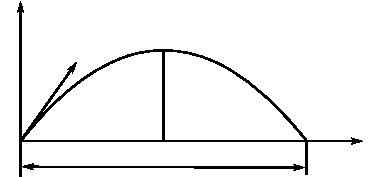
\includegraphics{figure/fig01.16}
    \caption{}
    \label{fig:01.16}
\end{wrapfigure}
因为当$\theta=\ang{45;;}$时,$\sin2\theta$
取最大值。所以,以同一速率$v_0$抛射物体,当
$\theta=\ang{45;;}$时,射程最远。
因为$\theta=\ang{90;;}$时,$\sin\theta$最
大,所以,只有当$\theta=\ang{90;;}$时,即竖直上抛,
$H$才能达到最大,其值为:
\begin{equation*}
    H_{\max }=\frac{v_{0}^{2}}{2 g}
\end{equation*}

这个题讨论的是理想情况,在实际情况中存在着空气阻力,
抛物速度愈大,阻力也愈大。空气阻力随着抛物速度的增加而逐
渐增加,在某一速度上将等于重力,这时物体将匀速下降。因而
实际上抛体的轨迹并不是理想的抛物线。

\section{圆周运动和角速度}\label{sec:01.09}

    现在来讨论一种最简单的曲线运动——圆周运动。即轨迹是
个圆。如果选择圆心作为坐标原点,质点的位置就可用位置矢量
$\vq{r}$与某一选定的方向(例如$X$轴)之间的夹角$\varphi$(图l·17)来描述,因
为$\varphi$确定之后,质点的位置就完全确定了。因而可用角$\varphi$与$t$的
关系$\varphi(t)$来代替函数$\vq{r}(t)$。

    我们知道,对于直线运动,用一个坐标$x(t)$就可以描写。同
样,对于圆周运动,也是只要一个坐标$\varphi(t)$来描写就够了。在这
个意义上,两者是一样的。而一般的平面曲线运动,需要两个坐
标来描写;一般的空间曲线运动,则需要三个坐标来描写。我
们按描写运动所需坐标的个数,把运动分为一维运动、二维运动、
三维运动等等。直线运动和圆周运动都是一维运动。

按照\ref{sec:01.07}节的讨论,速度的
方向为轨迹上相应点的切线方向,圆的切线总与半径相垂直,所
以圆周运动的速度$v$总与位置矢量$\vq{r}$相垂直。现在来求速度的大
小。由图l·18,在$t$时刻,质点位于$\varphi(t)$;当$t+\Delta t$时,位于
$\varphi(t+\Delta t)$,所以在$\Delta t$间隔中质点
运动的路程为:
\begin{equation*}
    \begin{aligned}
        \Delta s &=r|\varphi(t+\Delta t)-\varphi(t)| \\
        &=r|\Delta \varphi|
    \end{aligned}
\end{equation*}
将此式代入式\eqref{eqn:01.07.05}就得到圆周运动的速率
\begin{equation}\label{eqn:01.09.01}
    v=\lim _{\omega \rightarrow 0} \frac{r|\Delta \varphi|}{\Delta t}=r \lim _{\Delta \rightarrow 0} \frac{|\Delta \varphi|}{\Delta t}
\end{equation}
现在定义一个新的量,它是
\begin{equation}\label{eqn:01.09.02}
    \omega=\lim _{\Delta \rightarrow 0} \frac{|\Delta \varphi|}{\Delta t}
\end{equation}
这种形式的公式我们已经多次遇到了。$|\Delta\varphi|/\Delta t$是在$t$到$t+\Delta t$间
隔中,质点的单位时间的角位置的平均变化。当取$\Delta t\rightarrow 0$的极限
时,这个平均变化率过渡为瞬时变化率。因此,我们称$\omega$为角速
度,确切地说,应称为角速率。它的单位是弧度/秒。利用角速率$\varphi$,式\eqref{eqn:01.09.01}可以写成
\begin{equation}\label{eqn:01.09.03}
    v=r\varphi
\end{equation}

速度本质上是一个矢量,有大小和方向两方面。上述角速度
定义只反映了大小,为反映方向,我们需作些补充。

现在定义一个矢量$\omega$,它的大小等于式\eqref{eqn:01.09.01}中的$\omega$,$\omega$的
方向按图1·19所示的方法给定。

圈1·19角速度的方向
当我们从$\omega$指向的方向观察质点的运动时,质点总是沿逆时钟方
向转动。这个规定$\omega$的方向的方法也可以用一个正扣螺旋来说
明,当螺钉按质点运动方向旋转时,螺钉的运动方向就是$\omega$的方
向。

这样定义的$\omega$,称为角速度矢量。利用这个矢量。可以把质
点的速度矢量$\vq{v}$表示成
\begin{equation}\label{eqn:01.09.04}
    \vq{v}=\omega\times \vq{r}
\end{equation}
由图l。20,因为$\omega$与$\vq{r}$垂直,所以$|\omega\times\vq{r}|=\omega r=v$,
而且$|\omega\times\vq{r}|$的方向与$v$的方向一致。故式\eqref{eqn:01.09.04}
比\eqref{eqn:01.09.03}更具有一般性,它不仅表达了三者的大小关系,也反映了
三者间的方向关系。不仅如此,若取通过圆心且垂直于圆所在平面
的直线上任一点为原点(图l‘21)来描写圆周运动,式\eqref{eqn:01.09.04}仍成立,
但式\eqref{eqn:01.09.03}就不对了。读者可以自己证明。

图1.20圆周运动中0与v的关系  图1·21原点不在圆心的情况
\section{匀速圆周运动}\label{sec:01.10}

    一般情况角速率$\omega$是随$t$变化的,这时质点的速度的大小也
随$t$变化。以下讨论$\omega$不随$t$变化的特殊情况,即匀速圆周运动。
由式\eqref{eqn:01.09.03},这时质点的速率也不变化。质点绕圈周一圈走过的
路程是$2\pi r$。如果走一圈所用时间为$T$,则质点的速率是
\begin{equation}\label{eqn:01.10.01}
    v=\frac{2 \pi r}{T}
\end{equation}
T为周期,比较式\eqref{eqn:01.10.01}、\eqref{eqn:01.09.03},得到:
\begin{equation}\label{eqn:01.10.02}
    \omega=\frac{2 \pi}{T}, ~ T=\frac{2 \pi}{\omega}
\end{equation}
这也就是说,周期$T$等于质点转过$2\pi$角度所需要的时间。

    对于匀速圆周运动,$\vq{v}$的大小不变,而$\vq{v}$的方向时时在变,因
而它的加速度并不为零。由于速度方向总是垂直于矢量$\vq{r}$的,所
以在$t$到$t+\Delta t$间隔中,倘使$\vq{r}$转过角度$\Delta\varphi$,
则$\vq{v}$也就转过了$\Delta\varphi$。由于
$|\vq{v}(t)|=|\vq{v}(t+\Delta t)|=v$,由图\ref{fig:01.22}~的等腰三角形,得
\begin{equation*}
    \begin{aligned}
        |\vq{v}(t+\Delta t)-\vq{v}(t)| &=2 v \sin \frac{\Delta \varphi}{2} \\
        & \approx 2 v\frac{\Delta \varphi}{2}=v \Delta \varphi
    \end{aligned}
\end{equation*}

\begin{figure}[!h]
    \small\centering
    \begin{minipage}[b]{14em}
        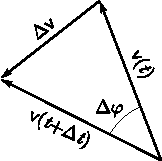
\includegraphics{figure/fig01.22}
        \vspace{1em}
        \caption{匀速圆周运动的加速度}
        \label{fig:01.22}
    \end{minipage}
    \begin{minipage}[b]{14em}
        \centering
        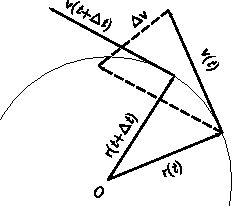
\includegraphics{figure/fig01.23}
        \caption{加速度的方向}
        \label{fig:01.23}
    \end{minipage}
\end{figure}
\noindent 将此式代入式\eqref{eqn:01.08.03},得
\begin{equation}\label{eqn:01.10.03}
    \begin{aligned}
        a & \equiv|\vq{a}|=\lim _{\Delta \rightarrow 0} \frac{|\vq{v}(t+\Delta t)-\vq{v}(t)|}{\Delta t} \\
        &=v\lim_{\boldsymbol{\alpha} \rightarrow 0} \frac{|\Delta \varphi|}{\Delta t}=v \omega=r \omega^{2}=\frac{v^{2}}{r}
    \end{aligned}
\end{equation}\vspace{0.5em}
上式推导中利用了式\eqref{eqn:01.09.02},\eqref{eqn:01.09.03}。因为$v$或$\omega$都不随$t$变,
所以匀速圆周运动的加速度的大小也不随$t$变,但它的方向是时
时变化的。根据图\ref{fig:01.23},当$\Delta t\rightarrow 0$时,
$\vq{v}(t+dt)-\vq{v}(t)=\Delta\vq{v}$的方
向趋于与$\vq{v}(t)$相垂直,并指向圆心。这样,匀速圆周运动的加速
度的大小由式\eqref{eqn:01.10.03}给出,而其方向总是指向圆心的。根据这
种方向上的特点,称这个加速度为向心加速度。

速度、角速度和加速度都是矢量,我们可把式\eqref{eqn:01.10.03}扩充
为矢量关系式:
\clearpage
~\vspace{-1.5em}
\begin{equation}\label{eqn:01.10.04}
    \vq{a}=\omega\times \vq{v}
\end{equation}
它的正确性也留给读者自己去证明。
\section{运动学里的反问题}\label{sec:01.11}

    以上各节讨论的问题,都是当已知运动的轨迹函数$\vq{r}(t)$后,
求速度和加速度。在运动学中还会遇到一种相反的问题:已知质
点在各时刻的速度$\vq{v}(t)$,求它的轨迹函数$\vq{r}(t)$;已知加速度$\vq{a}(t)$,
求它的$\vq{v}(t)$。以前各节讨论的问题多与微分运算相联系,而这些
反问题,却是与积分运算相联系的。

    仍然先讨论直线运动。如果已知直线运动的质点的速度为
$v(t)$,并已知在$t=0$时,质点在$x(0)$(称为初始位置),求在时刻
t的质点的坐标$x(t)$。

    我们把零到$t$这段时间间隔,分成许多小段,即$\Delta t_1$,$\Delta t_2$,$\cdots$,
而且$\Delta t_1+\Delta t_2+\cdots=t$,如果所有各小段都相当小,则在每个间隔
中速度变化不太大,在$\Delta t_i$中速度近似为$v(t_i)$。这样,在每个时
间间隔中质点的坐标变化分别近似为:
\begin{equation*}
    \begin{array}{l}
        \Delta x_{1} \approx v(t_{1}) \Delta t_{1} \\
        \Delta x_{2} \approx v(t_{2}) \Delta t_{2} \\
        \cdots \cdots
    \end{array}
\end{equation*}
因而,质点在0到$t$间隔中坐标的总变化$x(t)-x(0)$就应当等于
这许多小变化的总和,即\vspace{-0.5em}
{\setlength\abovedisplayskip{1pt}
\setlength\belowdisplayskip{1pt}
\begin{equation}\label{eqn:01.11.01}
    \begin{aligned}
        x(t)-x(0) &=\Delta x_{1}+\Delta x_{2}+\Delta x_{3}+\cdots \\
        & \approx \sum_{i} v\left(t_{i}\right) \Delta t_{i}
    \end{aligned}
\end{equation}}\vspace{-0.5em}
各时间间隔$\Delta t_i$取得越小,计算结果就越准确,当所有$\Delta t_i\rightarrow 0$时,
就得到质点位置变化的精确值:
\begin{equation}\label{eqn:01.11.02}
    x(t)=x(0)+\lim _{\Delta t_{i} \rightarrow 0} \sum_{i} v\left(t_{i}\right) \Delta t_{i}
\end{equation}
	上式取极限的项,与积分的定义是一样的。所以它可写成
\begin{equation}\label{eqn:01.11.03}
    x(t)=x(0)+\int_{0}^{t} v(t) d t
\end{equation}
这就是我们所要求的答案。

    现在说明式\eqref{eqn:01.11.01}或\eqref{eqn:01.11.02}中求和运算的几何意义。我
们在图l·24 中画出了速度$v$对时间$t$的关系曲线。各时间间隔$\Delta t_1$,$\Delta t_2$,$\cdots$,相应于横坐标上的各小段,各$v(t_1)$,$v(t_2)$,$\cdots$,相应
于各小段中v的近似值。因而$\Delta x_1$,$\Delta x_2$,$\cdots$,在数值上就等于相
应的小长方形的面积。故对所有$\Delta x_i$求和,在各小段$\Delta x_i$都趋于
无限小的情况下,在数值上就等于零到$t$间横轴之上与曲线$v$之
下所围的面积。

    利用这种几何性质,对一些简单情况,计算式\eqref{eqn:01.11.03}中的
积分是很容易的。下面举两个例子。
\begin{figure}[!h]
    \begin{minipage}[b]{14em}
        \centering
        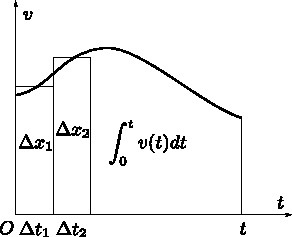
\includegraphics{figure/fig01.24.pdf}
        \caption{运动的$v-t$图}
        \label{fig:01.24}
    \end{minipage}\hfill
    \begin{minipage}[b]{14em}
        \centering
        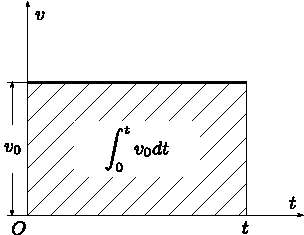
\includegraphics{figure/fig01.25.pdf}
        \caption{匀速运动的$v-t$图}
        \label{fig:01.25}
    \end{minipage}
\end{figure}

\example 匀速运动。

如果质点的速度是常数$v_0$,它的$v-t$图就如图l·25所示。由0
到$t$的横轴与曲线$v$围成一个长方形,它的面积是$v_0t$,将之代入
式\eqref{eqn:01.11.03},即得轨迹函数为:
\begin{equation}\label{eqn:01.11.04}
    x(t)=x(0)+v_0 t
\end{equation}
~\vspace{-1.5em}
\begin{figure}[!h]
    \begin{minipage}[b]{14em}
        \centering
        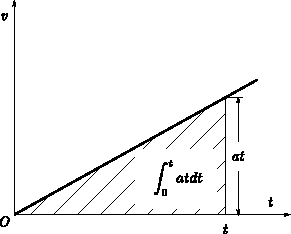
\includegraphics{figure/fig01.26.pdf}
        \caption{匀加速运动的$v-t$图}
        \label{fig:01.26}
    \end{minipage}\hfill
    \begin{minipage}[b]{14em}
        \centering
        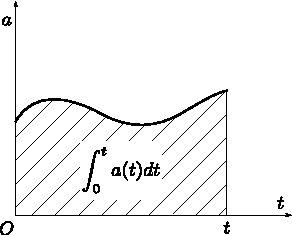
\includegraphics{figure/fig01.27.pdf}
        \caption{运动的$a-t$图}
        \label{fig:01.27}
    \end{minipage}
\end{figure}

  \vspace{-1em}\example 匀加速运动。

  设质点的速度与时间成正比,$v=at$,在图1·26中画出这个
关系。零到$t$的横轴与曲线$v$围成一个直角三角形,它的面积是
$\dfrac{1}{2} a t^2$,代入式\eqref{eqn:01.11.03},就得到轨迹函数为:
\begin{equation*}\label{eqn:01.11.04i}
    x(t)=x(0)+\frac{1}{2}at^2 \tag{1.11.4$'$}
\end{equation*}

    已知加速度$a(t)$,求速度$v(t)$的方法,同样可以按上面的方
法求得,将0到$t$的时间间隔分成小段$\Delta t_1$,$\Delta t_2$,$\cdots$,每个小段中
加速度分别近似为$a(t_1)$,$a(t_2)$,$\cdots$,因而在每个小段中,速度的
变化相应为$\Delta v_1\approx a(t_1)\Delta t_1$,$\Delta v_2\approx a(t_2)\Delta t_2$,$\cdots$,在0到$t$间隔中速
度总的变化等于所有变化之和,即
\begin{equation}\label{eqn:01.11.05}
    \begin{aligned}
        v(t)-v(0) &=\Delta v_{1}+\Delta v_{2}+\cdots \\
        & \approx \sum_{i} a\left(t_{i}\right) \Delta t_{i}
    \end{aligned}
\end{equation}
其中$v(0)$是$t=0$时质点的速度,称为初速度。
同样,取所有$\Delta t\approx 0$的极限,就得到速度变化的精确表达式为,
\begin{equation}\label{eqn:01.11.06}
    \begin{aligned}
        v(t) &=v(0)+\lim _{\Delta t_{i} \rightarrow 0} \sum a(t_{i}) \Delta t_{i} \\
        &=v(0)+\int_{0}^{t} a(t) d t
    \end{aligned}
\end{equation}
上式中积分的几何意义是$a-t$图中由0到$t$的横轴与$a$曲线之间
所围的面积(图1·27)。

    对于曲线运动的情况,式\eqref{eqn:01.11.03}、\eqref{eqn:01.11.06}分别推广成
{\setlength{\mathindent}{4em}
\setlength\abovedisplayskip{0pt}
\setlength\belowdisplayskip{0pt}
\setlength{\lineskip}{-1pt}
\setlength{\lineskiplimit}{-1pt}
\begin{eqnarray}
    \label{eqn:01.11.07}
    \begin{aligned}
        \vq{r}(t)=& \vq{r}(0)+\int_{0}^{t} \vq{v}(t) d t \\
        =& \vq{r}(0)
        +\left(\int_{0}^{t} v_{x}(t) d t\right) \vq{i}
        +\left(\int_{0}^{t} v_{y}(t) d t\right) \vq{J}  \\
        &+\left(\int_{0}^{t} v_{z}(t) d t\right) \vq{k}
    \end{aligned} \\
    \label{eqn:01.11.08}
    \begin{aligned}
        \vq{v}(t)=& \vq{v}(0)+\int_{0}^{t} \vq{a}(t) d t \\
        =& \vq{v}(0)
        +\left(\int_{0}^{t} a_{x}(t) d t\right) \vq{i}
        +\left(\int_{0}^{t} a_{y}(t) d t\right) \vq{J} \\
        &+\left(\int_{0}^{t} a_{z}(t) d t\right) \vq{k}
    \end{aligned}
\end{eqnarray}
\setlength{\mathindent}{6em}}%
其中$\vq{r}(0)$及$\vq{v}(0)$分别为初始时刻质点的位置矢量及速度矢量。具
体使用式\eqref{eqn:01.11.07}及\eqref{eqn:01.11.08}时,可以把它们分解成分量的关系
来计算。式\eqref{eqn:01.11.07}等价于下列三式。
{\setlength\abovedisplayskip{0pt}
    \setlength\belowdisplayskip{0pt}
    \setlength{\lineskip}{-1pt}
    \setlength{\lineskiplimit}{-1pt}
\begin{equation}
    \begin{aligned}\label{eqn:01.11.09}
        x(t)=x(0)+\int_{0}^{t} v_{x}(t) d t \\
        y(t)=y(0)+\int_{0}^{t} v_{y}(t) d t \\
        z(t)=z(0)+\int_{0}^{t} v_{z}(t) d t
    \end{aligned}
\end{equation}}%
而式\eqref{eqn:01.11.08}等价于下列三式。
{\setlength\abovedisplayskip{0pt}
    \setlength\belowdisplayskip{0pt}
    \setlength{\lineskip}{-1pt}
    \setlength{\lineskiplimit}{-1pt}
\begin{equation}\label{eqn:01.11.10}
    \begin{aligned}
        v_x(t)=v_x(0)+\int_{0}^{t} a_{x}(t) d t \\
        v_y(t)=v_y(0)+\int_{0}^{t} a_{y}(t) d t \\
        v_z(t)=v_z(0)+\int_{0}^{t} a_{z}(t) d t
    \end{aligned}
\end{equation}}%
这些积分中没有出现矢量,就可以按一一般方法计算,譬如上述的
面积方法就是一种可行的方法.

    研究运动有两种次序。一种是先研究轨迹,已知轨迹函数为
$\vq{r}(t)$,再来推求速度$\vq{v}(t)$,加速度$\vq{a}(t)$。就人类的认识过程来说,的
确是先看到轨迹的形状,然后有了运动快慢的概念,最后认识到
速度的变化,即加速度。另一种次序是:先知道加速度,然后再
求速度及轨迹。在物理学中,从力学的规律来看。往往是如此。

    前一种次序,看上去非常自然,是人类研究机械运动所走的
一条路。在牛顿之前,亚里士多德认为轨迹是最基本的,速度则
次之。这种方法的特点是先研究运动的大的整体方面,然后再涉
及局部细节。

    后一种次序,是牛顿创建的方法。也是现代物理学一个基本
的方法。牛顿认为,不要先探讨物体运动的整体方面。而是先研
究运动的瞬时情况,瞬时情况更为基本。弄清瞬时情况之后再来
讨论整体运动。也可以说,这种方法是先研究局部细节,然后再
作积分,得到整体性质。至今在大多数情况下,物理学家仍采取
牛顿的这种方法。

    上述两种方法反映了两种不同的信念。一种认为整体的大的
方面更简单些,因此,主张从大到小的研究顺序;另一种认为局
部的单元过程更简单些,因此。主张从小到大的研究顺序。我们
将在第五章说明,这两种“简单性”可能是分不开的。
\questions
\fangsong
\question 一个原则上不能进行直接或间接测量的物理量是否有意
义?

\question 平均速率有两种意思,一是指平均速度矢量的大小,一
是指物体运动路径总长度除以所用的总时间。这两种意思是否相
同?

\question 质点作一维运动,如果加速度不是恒量,质点的平均速率
是否等于$\dfrac 1 2$(初速+末速)?

\question 当物体的加速度恒定不变时,它的运动方向可否改变?

\question 质点的运动方程为$x=x(t)$,$y=y(t)$。在计算它的速度和
加速度的大小时,有人先求出$r=\sqrt{x^2+y^2}$,然后根据$v=\dfrac{\diff r}{\diff t}$,
$a=\dfrac{\diff ^2r}{\diff t^2}$,求得结果;有人先计算速度和加速度分量,再合成,所
得结果为:\vspace{-1em}
\begin{equation*}
    \begin{aligned}
        v &=\sqrt{\left(\frac{\diff  x}{\diff  t}\right)^{2}+\left(\frac{\diff  y}{\diff  t}\right)^{2}} \\
        a &=\sqrt{\left(\frac{\diff ^{2} x}{\diff  t^{2}}\right)^{2}+\left(\frac{\diff ^{2} y}{\diff  t^{2}}\right)^{2}}
    \end{aligned}
\end{equation*}
你认为哪一组结果正确?

\question  两千多年前,住在尼罗河口亚历山大城的埃拉托色尼,首
估算出地球的半径。然而,真正沿着地球子午线用绳长及日晷对
地球进行测量的,却是中国唐代高僧一行(公元683$\sim$727)。你知
道高僧一行测量的原理,方法及计算结果吗?

\question  设想将一小球上抛。如不考虑空气阻力,试证明它返回原
地时的速率等于开始的速率,并证明上升和下落所经过的时间相
等。

\question  将一小球铅直地上抛,若考虑空气阻力,它上升和下降所
经过的时间哪一个长?

\question  假设有两石块$m$和$M$,其中$m$较轻,$M$较重。按照亚里士多
德的看法,在地面上$M$应该比$m$下落得快些。伽利略首先用思辨
的方式指出亚里士多德的看法是自相矛盾的。伽利略说,设想将
$m$与$M$系在一起,则构成物体$(m+M)$,此物下落时,因为$m$有下
落得较慢的趋势,所以,$m$应该阻碍$M$,使它下落得比$m$快些而又
比$M$慢些;但是另一方面,物体$(m+M)$比$M$还要重,按照亚里
士多德的看法,它应比$M$下落得更快。因此,导致矛盾。

你认为伽利略的推理是否正确?

\question  质点在空间的运动,一般是三维运动。忽略风的作用的抛
体运动,为什么可以作为二维运动来处理?
\normalfont

\exercises
\fangsong

\exercise 用芝诺时计算阿基里斯的速度$v_1'$和加速度$a_1'$,并给出$x-t'$图。

\exercise 甲乙两列火车在同一水平直路上以相等的速率(30公里/时)
相向而行。当它们相隔60公里的时候,一只鸟以60公里/时的
恒定速率离开甲车头向乙车头飞去,一当到达立即返回,如此来
回往返不止。试求:

(1)当两车头相遇时,鸟往返了多少次?

(2)鸟共飞行了多少时间及距离?

(3)我们定义一种特殊的“小鸟钟”:小鸟从一车头到另一车
头为小鸟钟的时间测量单位(即小鸟钟的一个“滴答”)。用小鸟
钟记时的数值为$t''$求$t''$与一般时钟记时$t$之间的变换。

\exercise 一人从$O$点出发,向正东走3.0米,又向正北走1.0米,
\begin{wrapfigure}[8]{r}{8.5em}
    \begin{center}
        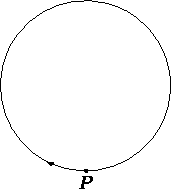
\includegraphics{figure/fig01.28}
        \caption{}
        \label{fig:01.28}
    \end{center}
\end{wrapfigure}
然后向东北走2.0米,试求合位移的大小及方向。

\exercise 一质点从$ P $出发,向左以匀速率1.0厘米/秒沿半径为$R=1.0$米的圆周运动(图\ref{fig:01.28})。问:

(1)当它走过2/3圆周时,位移是多少?走过的路程是多少?在这段时间内的
平均速度是多少?该点的瞬时速度是多少?

\clearpage
(2)当它走过1/2圆周时,以上各值又如何?

\exercise 一物体作直线运动,它的位置由方程$x=10t^2+6$决定,其
中$x$的单位为厘米,$t$的单位为秒,试计算:

(1)在3.00~3.10秒、3.000~3.01秒及3.000~3.001秒间
隔内的平均速度,

(2)在$t=3.00$秒时的瞬时速度;

(3)用微分方法求它的速度及加速度公式。

\exercise 有一质点沿x方向作直线运动,t时刻的坐标为:\\
\null\qquad\qquad \qquad $x=4.5t^2-2t^3$\\
式中$x$的单位为米。$t$的单位为秒。试求:

(1)第2秒内的位移和平均速度;

(2)第1秒末和第2秒末的瞬时速度;

(3)第2秒内质点所走过路径的长度;

(4)第2秒内的平均加速度以及第0.5秒末和第1秒末的瞬时
加速度。

\exercise 一质点以恒定的径向速度$r=4$米/秒在一平面中运动。它
的角速度为常量,其大小为$\omega=\dot\theta=2$弧度/秒。当质点距原点为3
米时,它的速度的大小及加速度大小是多少?

{
\exercise 如图\ref{fig:01.29}~所示,向上抛一物体,测量物体上抛及下落经
\begin{wrapfigure}[8]{r}{12.5em}
    \vspace{1em}
    \begin{center}
        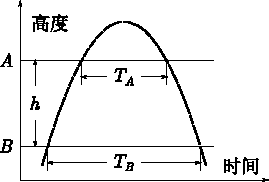
\includegraphics{figure/fig01.29}
        \caption{}
        \label{fig:01.29}
    \end{center}
\end{wrapfigure}
过水平线$A$的时差$T_A$,以及上抛
及下落经过水平线$B$的时差$T_B$。
试证明,若忽略空气阻力,重力
加速度的大小可以表示为:\\
\null\hspace{3em}$g=\dfrac{8h}{T_A^2 - T_B^2}$ \\
式中$h$是$B$线与$A$线的高度差。}

\exercise 天体物理常涉及大尺度的\\
问题,为了方便起见,引进一些
\clearpage
\noindent 实用的大的长度单位。一个天文单位(AU)等于从地球到太阳的
平均距离;一个秒差距是一个天文单位所张之角为1秒的距离,即
观测者从某一恒星看地球公转轨道半径所张的角度为1秒时,该恒
星与太阳之间的距离。试求。

(1) 1秒差距相当于多少米?多少天文单位?及多少光年?

(2)以秒差距为单位,表示地球到太阳的距离。

\exercise 一物体从离地面的高度为$ h $的地方,由静止开始自由下
落,经过最后196米所用的时间是4.0秒钟。求物体下落过程所用
的总时间及其高度。

\exercise 一枚从地面发射的火箭以20米/$\text{秒}^2$的匀加速度竖直上升
半分钟后,燃料用完,于是象一个自由质点一样运动。略去空气
阻力,试求。

(1)火箭达到的最大高度;

(2)它从离开地面到再回地面所经过的总时间。

\exercise 把两个小物体从同一地点以同样初速率$v_0=24.5$米/秒
先后竖直上抛,设抛出两物体的时差为$\Delta t=0.500$秒,试问:

\renewcommand{\hsp}{\hspace{0.2em}}
{(1)\ziju{-0.015}第二个物体抛出后,经过多少时间\hsp $t$\hsp 才与第一个物体相遇?}

\vspace{-0.15em}(2)如果$\Delta t\geqslant\dfrac{2v_0}{g}$,讨论结果的物理意义。\vspace{-0.15em}

\exercise 物体以初速$v_0=20$米/秒被抛出,抛射仰角是\ang{60;;},略去
空气阻力,试问:

(1)物体开始运动后的1.5秒末,运动方向与水平方向的夹角
$\alpha$是多少?2.5秒末夹角$\alpha$又为多少?

(2)物体抛出后经过多少时间,运动方向才与水平成\ang{45;;}角?
这时物体的高度是多少?

(3)在物体轨迹最高点处的曲率半径$R_1$有多大?

(4)在物体落地点处,轨迹的曲率半径$R_2$有多大?

\exercise 高台下降滑雪在一平滑的山坡上进行。山坡与水平线成
恒定角度$\alpha$,滑雪运动员初速率为$v_0$,并以与水平线成$\theta$的仰角跳
出(\ref{fig:01.30})。若不考虑空气阻力,试证明:
\begin{figurex}
    \centering
    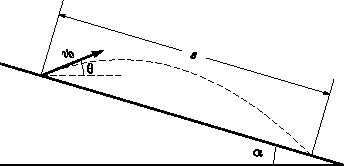
\includegraphics{figure/fig01.30}
    \caption{}
    \label{fig:01.30}
\end{figurex}

(1)运动员落在斜坡上的距离为:
\begin{equation*}
    s=\frac{2 v_{0}^{2} \sin (\theta+a) \cos \theta}{g \cos ^{2} \alpha}
\end{equation*}

(2)对于一定的$v_0$和$\alpha$来说,$s$在$\theta=\ang{45;;}-\dfrac{\alpha}{2}$时有最大值。其
值为:
\begin{equation*}
    s_{\max }=\frac{v_{0}^{2}(1+\sin \alpha)}{g \cos ^{2} \alpha}
\end{equation*}

\exercise 1977年中国男子铁饼的最好记录是54.28米,1983年提高
到60米。这些记录都是在北京创造的,北京的重力加速度$g$为
980.12厘米/$\text{秒}^2$。设投掷点比落地点高1.5米,略去空气阻力,
问投掷时至少要用多大的初速度,才可达到上述距离?

\exercise 设若干个光滑斜面($a_1$,$a_2$,$a_3$,…)有共同的底边$b$为30
厘米。试问:

(1)斜面与水平夹角$\alpha$为多大时,才能使物体在该斜面上从顶
端自由滑至底上正好需时为$t=0.4$秒?

(2)多大的夹角$\alpha$,使下滑的时间最短?

\exercise 在空间某一点$O$以相同的速率向各方向同时把若干小
球搬出去。试证明在略去空气阻力的情况下,任一时刻$t$,所有小
球都位于一个球面上,并求:

(1)此球心的运动方程式;

(2)球面距球心的距离。

\exercise 若抛射体的初速率为$v_0$,抛射角为$\theta$,略去空气阻力。伽
利略说:“抛射角为$\ang{45;;}+\delta$和$\ang{45;;}-\delta(\delta<\ang{45;;})$的两个抛射体初速
率相同时,射程是相等的。”试证明他的话,并证明$\theta=\ang{45;;}$时水
平射程最大。

\begin{wrapfigure}[8]{r}{12.5em}
    \vspace{-2.5em}
    \begin{center}
        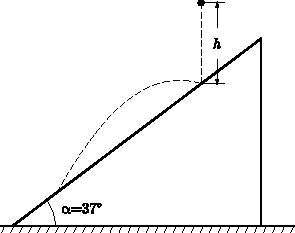
\includegraphics{figure/fig01.31}
        \caption{}
        \label{fig:01.31}
    \end{center}
\end{wrapfigure}
\exercise 一弹性球自由下落在一斜面上,与斜面发生完全弹性碰
撞,下落高度$h=20$厘米,斜面对水平的倾角$\alpha=\ang{37;;}$(图\ref{fig:01.31})。若
不计空气阻力,它第二次碰到斜面的位置距原来的下落点多远?

\exercise 用枪瞄准空中的靶,当子弹射出枪口时,靶同时自由下
落。如果略去空气阻力。不论子弹速率多大,总会击中下落的靶,
这个现象叫做百发百中,说明其中理由。

\exercise 一轰炸机高海面10公里,以240公里/小时的水平速度追
击正前方一鱼雷艇,鱼雷艇的速度是95公里/小时,不计空气阻
力,问飞机应在艇后多少距离投弹才能正好击中目标?

\exercise 一俯冲轰炸机沿与铅垂线成$\ang{37;;}$方向俯冲,在800米高度
投弹,炸弹离开飞机5.0秒钟时着地。不计空气阻力,试问:

(1)飞机的飞行速度是多少?

(2)炸弹离开飞机后在水平方向前进多远?

(3)炸弹着地时,速度的大小和方向?

\exercise 应以多大的水平速度$v$把一物体从高$h$处抛出,才能使
它在水平方向的射程为$h$的$n$倍?

\exercise 飞机以360公里/小时的速度由东向西飞行。试回答:

(1)在什么地理纬度上,飞机上的人可以看见太阳不动地停
在空中?

(2)若在极地附近沿纬线以圆轨道由东向西飞行,可以看见
什么现象?

\exercise 一俯冲轰炸机以不变的速率450公里/小时俯冲后。急离
俯冲线改为沿一铅垂平面内的圆形路线飞行。试问:要使飞机在
圆的最低点的加速度不超过$7g$,圆形路线的最小半径应是多少?

\exercise 车轮在地平面上作匀角速的纯滚动,轮行的速度为$v_0=
10$米/秒,轮的半径为$r=0.50$米,试求;

(1)车轮边缘上一点$A$的角速度$\omega$;

(2)$A$点的轨迹。

\exercise 一半径为$r$的小球沿两固定的等高平行导轨作纯滚动,
两导轨间的距离为$d$,如图\ref{fig:01.32}~所示。试问:

(1)球心的速度与球的角速度的关系是怎样的?

(2)小球面上一点$A$的轨迹如何?
\begin{figurex}
    %\vspace{-1em}
    \begin{center}
        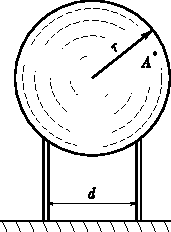
\includegraphics{figure/fig01.32}
        \caption{}
        \label{fig:01.32}
    \end{center}
\end{figurex}

\normalfont

% 第二章
\setcounter{chapter}{1}
\chapter{运动学中的相对性}\label{chp:02}

\section{相对和绝对}

人对自然界认识的深化,常常是和弄清什么是相对的、什么
是绝对的这类问题联系在一起的。

远古时期,无论在东方文明或西方文明中,都认为大地是平
坦的,天在大地的上面。“天圆地方”就是这种观念的通俗表
述。用现代语言来说,在这种观念中,“上”“下”这两个方向是
绝对的。

到古希腊时期,毕达哥拉斯以及亚里士多德等先后开始主张
大地是一个球体,即地球。中国的“浑天说”也有大体相似的观
念。这是认识上的一次进步,因为它抛弃了当时的一种“习惯”
的但却不正确的观念——“上”“下”是绝对的。

按照当时“习惯”的看法,如果大地是球形,那些居住在我们
的对蹠点上的人不是早就“掉下”去了吗?可见,树立球形大地
观需要克服一些不正确的成见所带来的阻力。因此,从相对与绝
对角度来评价,可以说,地球观是把“上”和“下”这两个方向
相对化了。我们看对照点的人在“下”,对照点的人看我们也是
在“下”,亦即空间各个方向是等价的,没有一个方向具有特别
的绝对优越的性质。

在亚里士多德的体系中,认为地球的球心是宇宙的中心。这
个位置具有非常特殊的,绝对的意义。亚里士多德还认为,物体
运动的规律是力图达到自己的天然位置,地面附近物体的天然位
置就是地球的中心,远处物体(如星体)则应环绕着地球的中心。
这样,在支配物体运动的规律中,空间位置具有特别的作用,这
种性质,可以叫做空间位置的绝对性。

以牛顿力学为起点的物理学,否定了亚里士多德体系中的空
间位置的绝对性,认为任何的空间点都是平权的,地心在宇宙中
并不占有特殊的地位。牛顿理论中的相对和绝对,又不同于亚里
士多德了。

正因为相对和绝对这一问题的重要性,在这一章里,我们将
系统地分析一下牛顿的运动学中的相对性,并且还将指出,牛顿
体系中的相对绝对观也是有局限的,在某些条件下,就完金不适
用了。
\section{位置和轨迹的相对性}\label{sec:02.01}
在运动学中,最基本的概念是位置。由图2·l看到。对于质点
$P$,相对于参考系$K$而言,它的位置矢量是$OP$,即
\begin{equation*}
    \vq{OP}=x\vq{i}+y\vq{j}+z\vq{k}
\end{equation*}
同时,相对于参考系$K'$来说,它的位置矢量是$O'P$,即
\begin{equation*}
    \vq{O'P}=x'\vq{i'}+y'\vq{j'}+z'\vq{k'}
\end{equation*}
\begin{figurex}
    \centering
    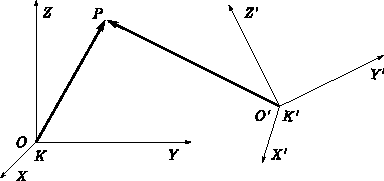
\includegraphics{figure/fig02.01}
    \caption{位置的相对性}
    \label{fig:02.01}
\end{figurex}

可见同一质点的位置,对不同的参考系,可用不同的位置矢量来
描写,这就是位置描写中的相对性。

从描写质点位置来说,选用参考系K或者K',是等价的。因
为参考系$K$及$K'$一旦选定,它们之间的关系就完全确定了。我们
知道了质点在参考系$K$中的位置坐标$(x,y,z)$,就可求得在参考
系$K'$中的位置坐标$(x,y,z)$,反之亦然。用数学语言来说,
即$x$,$y$,$z$与$x'$,$y'$,$z'$之间有确定的变换关系:
\begin{align}
    \label{eqn:02.02.01}
    &\left\{\begin{array}{l}
        x'=x'(x, y, z) \\
        y'=y'(x, y, z) \\
        z'=z'(x, y, z)
    \end{array}\right. \\
    \label{eqn:02.02.02}
    &\left\{\begin{array}{l}
    x=x(x', y', z') \\
    y=y(x', y', z') \\
    z=z(x', y', z')
    \end{array}\right.
\end{align}
式\eqref{eqn:02.02.01}、\eqref{eqn:02.02.02}~称为坐标变换。

现在我们介绍几种物理学中常用的坐标变换。

\begin{wrapfigure}{r}{16em}
    \centering
    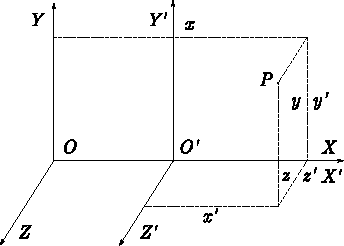
\includegraphics{figure/fig02.02}
    \caption{空间平移}
    \label{fig:02.02}
\end{wrapfigure}
\heiti 1. 坐标平移 \normalfont

如图\ref{fig:02.02},参考系$K$及$K'$的$X$轴与$X'$轴重合,$Y$轴与$Y'$轴平行,
$Z$轴与$Z'$轴平行,原点$P$的坐标在参考系$K$及$K'$中分别是$x$,$y$,$z$和
$x'$,$y'$,$z'$,显然,坐标变换是:\vspace{-0.2em}
\begin{equation}\label{eqn:02.02.03}
    \left\{\begin{array}{l}
        x=x'+d \\
        y=y' \\
        z=z'
    \end{array}\right.
\end{equation}

\begin{wrapfigure}{r}{15em}
    \centering
    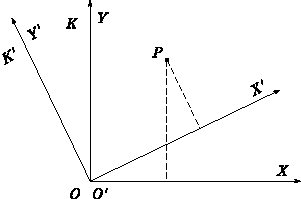
\includegraphics{figure/fig02.03}
    \caption{空间转动}
    \label{fig:02.03}
\end{wrapfigure}
\heiti 2. 坐标转动 \normalfont

讨论平面问题时,取如图\ref{fig:02.03}~的参考系$K$及$K'$,它们的原点$O$与$O'$重合,参考
系$K'$的轴相对于参考系K转动一个$\theta$角。质点$P$的位置坐标在参考系$K$,
$K'$中分别是$x$,$y$,$z$和$x'$,$y'$,$z'$。不难求出,此时的坐标变换是:\vspace{-0.2em}
\begin{equation}\label{eqn:02.02.04}
    \left\{\begin{array}{l}
        x=x'\cos\theta-y'\sin\theta \\
        y=x'\sin\theta+y'\cos\theta
    \end{array}\right.
\end{equation}
或\vspace{-1em}
\begin{equation*}
    \left\{\begin{array}{l}
        x'=x\cos\theta+y\sin\theta \\
        y'=x\sin\theta-y\cos\theta
    \end{array}\right.
\end{equation*}

\begin{wrapfigure}{r}{15em}
    \centering
    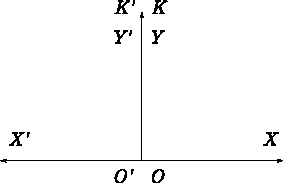
\includegraphics{figure/fig02.04}
    \caption{空间反演}
    \label{fig:02.04}
\end{wrapfigure}
\heiti 3. 空间反演 \normalfont

如图\ref{fig:02.04},参考系$K$与$K'$的原点$O$与$O'$重合,$Y$轴与$Y'$轴重合,而$X$轴与
$X'$轴反向。这时,坐标变换是:\vspace{-0.5em}
{\setlength{\mathindent}{2em}
\begin{equation}\label{eqn:02.02.05}
    \left\{\begin{array}{l}
        x=-x' \\
        y=y
    \end{array}\right.
\end{equation}}%
弄清了位置的相对性,关于轨迹的相对性也就不难理解了。
质点运动的轨迹,一般来说是一条空间曲线。对于一个质点
的轨迹,相对于参考系K,我们可用曲线方程
\begin{equation}\label{eqn:02.02.06}
    \left\{\begin{array}{l}
        f_1(x,y,x)=0 \\
        f_2(x,y,z)=0
    \end{array}\right.
\end{equation}
来描写;也可相对于参考系$K'$,用曲线方程

~\vspace{-1.56em}
\begin{equation}\label{eqn:02.02.07}
    \left\{\begin{array}{l}
        f'_1(x',y',x')=0 \\
        f'_2(x',y',z')=0
    \end{array}\right.
\end{equation}
来描写。一般说来,函数形式$f_1$,$f_2$和式$f'_1$,$f'_2$是不相同的,这
就是轨迹的相对性。将式\eqref{eqn:02.02.02}~代入式\eqref{eqn:02.02.06},就可由$f$求得
$f'$;将式\eqref{eqn:02.02.01}~代入式\eqref{eqn:02.02.07},就可由$f'$求得$f$。

作为示例,我们讨论两个平面运动。有两个质点。它们相对
于参考系$K$的运动轨迹分别由下列曲线方程描写:
\begin{align}
        x-ky&=0  \label{eqn:02.02.08}\\
    x^2+y^2&=r^2 \label{eqn:02.02.09}
\end{align}
式\eqref{eqn:02.02.08}~表示一直线运动,式\eqref{eqn:02.02.09}~表示中心在原点,半径
为$r$的一个圆周运动。

现在取另一参考系$K'$,它仅相对于参考系$K$转了一个$\theta$角。
我们把式\eqref{eqn:02.02.04}代入式\eqref{eqn:02.02.08},整理后得
{\setlength{\mathindent}{4em}
\begin{equation}\label{eqn:02.02.10}
    x'(\cos\theta - k\sin\theta)-y'(\sin\theta + k\cos\theta)=0
\end{equation}}%
式\eqref{eqn:02.02.10}~就是在参考系$K'$中所看到的第一个质点的轨迹方程,
它也是一条直线,但斜率与式\eqref{eqn:02.02.08}不同。
将式\eqref{eqn:02.02.04}~代入式\eqref{eqn:02.02.09},得
\begin{equation}\label{eqn:02.02.11}
    x'^2+y'^2=r^2
\end{equation}
由式\eqref{eqn:02.02.11}~看到,第二个质点的轨迹相对于参考系$K'$,也是中
心在原点。半径为$r$的圆。
如果一种运动轨迹相对于两参考系形状相同。而且它与两坐
标系的关系也一样,我们称这种特殊轨迹对于这一特定的坐标变
换具有不变性。用数学语育来说,当参考系$K$变到$K'$时。若轨迹
方程由
\begin{equation*}
    f(x,y,z)=0
\end{equation*}
变换成
\begin{equation*}
    f(x',y',z')=0
\end{equation*}
它就是具有不变性的轨迹。由此可见,第一个质点轨迹相对于坐
\clearpage
\noindent 标转动变换并不具有不变性,而第二个质点轨迹对于坐标转动变
换是有不变性的。

下面讨论涉及时间的变换,坐标系$K$及$K'$所用的时间$t$及$t'$
也可以是不相同的。最常遇到的一种时同变换,是所谓时间平移,
即$t=t'+t_0$,也就是$K$及$K'$的时间坐标的原点相差一常数$t_0$。
譬如,在参考系$K$中用东京时间,在参考系$K'$中用北京时间,
那么,常数$t_0$就等于1小时。

如果在参考系K中,轨迹函数是\vspace{-0.2em}
\\\null\qquad\qquad\qquad$x=x(t)$
\\\null\qquad\qquad\qquad$y=y(t)$
\\\null\qquad\qquad\qquad$z=z(t)$\\
我们很容易推知,在参考系$K'$中,轨迹函数是\vspace{-0.2em}
\\\null\qquad\qquad\qquad$x=x(t'+t_0)$
\\\null\qquad\qquad\qquad$y=y(t'+t_0)$
\\\null\qquad\qquad\qquad$z=z(t'+t_0)$

另一种时间变换在日常生活中不常见,但在物理上非常有用。
那就是\vspace{-0.5em}
\\\null\qquad\qquad\qquad$t=-t'$\\
它表示当$K$中的时间走向将来时,$K'$相应的时间却走向过去。因
此,称这种时间变换为时间倒转。

我们不难由参考系$K$中的轨迹函数\vspace{-0.2em}
\\\null\qquad\qquad\qquad$x=x(t)$
\\\null\qquad\qquad\qquad$y=y(t)$
\\\null\qquad\qquad\qquad$z=z(t)$\\
得到相应在参考系$K'$中的轨迹函数为\vspace{-0.2em}
\\\null\qquad\qquad\qquad$x=x(-t')$
\\\null\qquad\qquad\qquad$y=y(-t')$
\\\null\qquad\qquad\qquad$z=z(-t')$

为了弄清时间倒转的物理意义,我们举一个直线运动的例子
(图\ref{fig:02.05})。质点沿$X$轴运动。在参考系$K$中看,$t=1$时,质点在$x_1$;
$t=2$时,在$x_2$;显然,质点是从左向右运动的。但在参考系$K'$中看,
质点在$x_1$时,$t'=-1$;在$x_2$时。$t'=-2$,由于时间$t'=-2$比$t'=-1$
早,而时间总是从过去向将来发展,因此,相对于参考系$K'$,质
点是从右向左运动的。
\begin{figurex}
    \centering
    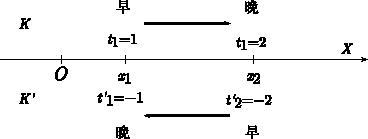
\includegraphics{figure/fig02.05}
    \caption{时间倒转}
    \label{fig:02.05}
\end{figurex}

\section{速度的相对性}\label{sec:02.03}
    我们首先讨论质点的直线运动.

    取参考系$K$和$K'$的$X$轴都和质点轨迹重合,而两原点$O$、$O'$
相距为$d$(图\ref{fig:02.06})。由式\eqref{eqn:02.02.03}知,$K$,$K'$之间的坐标变换是
    \begin{equation*}
        x'=x-d
    \end{equation*}
现在,若$K'$相对于$K$以均匀速率$u$沿$X$正向运动,则有
    \begin{equation*}
        d=ut+d_0
    \end{equation*}
\vspace{-1.56em}
\begin{figurex}[!h]
    \centering
    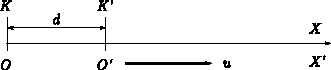
\includegraphics{figure/fig02.06}
    \caption{速度的相对性}
    \label{fig:02.06}
\end{figurex}

\noindent 其中$d_0$是时间$t=0$时,坐标原点$O$,$O'$间的距离。故坐标变换
公式为

~\vspace{-2em}
\begin{equation}
    x'=x-ut-d_0 \label{eqn:02.03.01}
\end{equation}

有了式\eqref{eqn:02.03.01},就不难讨论$K$,$K'$之间的变换关系。

设在$K$系中,质点轨迹函数为
\begin{equation*}
    x=x(t)
\end{equation*}
根据定义,质点相对于K系的速度为
\begin{equation*}
    v(t)\equiv\frac{\dif x}{\dif t}
\end{equation*}

相对于$K'$系,由式(2.3.1),质点的轨迹函数应为
\begin{equation*}
    x'=x'(t)=x(t)-ut-d_0
\end{equation*}
按照定义,质点相对于$K'$的速度为
\begin{equation*}
    \erratanote{\ensuremath{v(t)}}{原书漏印“$v$”。}\equiv\frac{\dif x'}{\dif t}=\frac{\dif x}{\dif t}-u
\end{equation*}
即\vspace{-1.7em}
\begin{equation}
    v'=v-u \label{eqn:02.03.02}
\end{equation}
式\eqref{eqn:02.03.02}就是同一质点相对于$K$及$K'$二者的速度之间的关系。

\begin{wrapfigure}[10]{r}{14.5em}
    \centering
    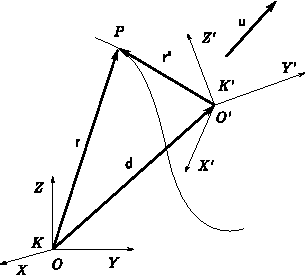
\includegraphics{figure/fig02.07}
    \caption{相对作匀速运动的$K$及$K'$}
    \label{fig:02.07}
\end{wrapfigure}
现在把式\eqref{eqn:02.03.02}推广到三维情况。

由图\ref{fig:02.07}~知,在$K$及$K'$中,质点$P$的位置分别用$\vec{r}$,
$\vec{r'}$表示。它们之间的关系是
{\setlength{\mathindent}{4em}
\begin{equation*}
    \vec{r'}=\vec{r}-\vec{d}
\end{equation*}}%
如果$K'$系相对于$K$系以均匀速度$\vec{u}$运动,则有
{\setlength{\mathindent}{4em}
\begin{equation*}
    \vec{d}=\vec{u}t+\vec{d}_0
\end{equation*}}%
其中$\vec{d}_0$是时刻$t=0$时,从\\$O$到$O'$的矢量。故有
\begin{equation}
    \vec{r}'=\vec{r}-\vec{u}t-\vec{d}_0 \label{eqn:02.03.03}
\end{equation}
若在$K$系中,质点的轨迹函数是
\begin{equation*}
    \vec{r}=\vec{r}(t)
\end{equation*}
则根据定义,质点相对于$K$的速度是
\begin{equation}\label{eqn:02.03.04}
    \vec{v}(t)\equiv\frac{\dif \vec{r}}{\dif t}
\end{equation}
另一方面,由式\eqref{eqn:02.03.03}~可以求出质点在$K'$系中的轨迹函数,它是\vspace{-1em}
\begin{equation*}
    \erratanote{\ensuremath{\vec{r}'=}}{原书作“$\vec{r}=\dots$”,显误。}\vec{r}'(t)=\vec{r}(t)-\vec{u}t-\vec{d}_0
\end{equation*}
因此,质点相对于$ K' $的速度是
\begin{equation}\label{eqn:02.03.05}
    \vec{v}'(t)\equiv\frac{\dif \vec{r}'}{\dif t}=\frac{\dif \vec{r}}{\dif t}-\vec{u}
\end{equation}
即\vspace{-2em}
\begin{equation}\label{eqn:02.03.06}
     \vec{v}'=\vec{v}-\vec{u}
\end{equation}
式\eqref{eqn:02.03.06}~就是三维情况的速度变换公式,又称速度合成公式。可
见,在不同参考系中,同一运动可能具有不同速度,亦即速度是
具有相对性的概念。

\begin{wrapfigure}{r}{17em}
    \vspace{-1em}
    \centering
    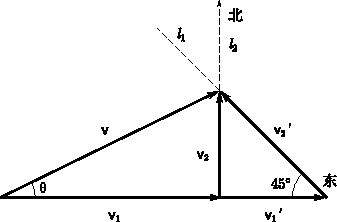
\includegraphics{figure/fig02.08}
    \caption{}
    \label{fig:02.08}
\end{wrapfigure}
\example 一人向东以$v_1=50\text{米/分}$的速度运动,他觉得风从正南
方吹来。假若人行速度增至$v_1'=75\text{米/分}$,他觉得风从东南方吹来。
求风的速度$\vec{v}$。

\solution 设两次感觉到的风速为$\vec{v}_2$和$\vec{v}_2'$。根据题意,各个速度应有以下关系:
\begin{align*}
    \vec{v}_1+\vec{v}_2=\vec{v} \tag{1} \label{xeqn:02.03.01} \\
    \vec{v}_1'+\vec{v}_2'=\vec{v} \tag{2} \label{xeqn:02.03.02}
\end{align*}
作出矢量图(图\ref{fig:02.08})由式\eqref{xeqn:02.03.01}知$\vec{v}$的末端在$l_1$上,由式\eqref{xeqn:02.03.02}知$\vec{v}$的
末端在$l_2$上,故$l_1$和$l_2$的交点是$\vec{v}$的末端。显然有:
\begin{equation*}
        v_1=v_1'-v_1=76-50=25\text{米/分}
\end{equation*}

~\vspace{-1.2em}
\begin{align*}
    v&=\sqrt{v_1^2+v_2^2}=\sqrt{50^2+25^2}=25\sqrt{25}\text{米/分} \\
    \theta&=\arctg\frac{v_2}{v_1}=\arctg\frac{25}{50}=\ang{26;35;}
\end{align*}
从而可看到不同参考系中能感觉到不同的风速。在地球参考系中
风速是$\vec{v}$,以50米/分向东行走的人感觉风速是$\vec{v}_2$;而以75米/分向
东行走的人则感觉到风速是$\vec{v}_2'$。

\example 一列火车以速度$\vec{v}_1$沿水平直轨运行。车上有人以初
速度$\vec{v}_2$竖直向上抛出一小球。车上及地面各站一人研究小球的运
动。在不计空气阻力情况下,不同观察者看到速度,加速度及轨
迹有何不同?

\solution (1)以车为参考系。

因为\vspace{-1em}
\begin{align*}
    &\vec{v}=\vec{v}_x+\vec{v}_y=v_x\vec{i}+v_y\vec{j} \\
    &v_x=0,~ v_y=v_2-gt
\end{align*}
所以\vspace{-1em}
\begin{align*}
    &\vec{v}=(v_2-gt)\vec{j} \\
    &|\vec{v}|=v_2-gt
\end{align*}
运动在铅直线上进行,是竖直上抛运动;加速度是重力加速度$g$。

(2)以地心为参考系。

因为\vspace{-1em}
\begin{equation*}
    \vec{v}=\vec{v}_x+\vec{v}_y=v_1\vec{i}+(v_2-gt)\vec{j}
\end{equation*}
故\vspace{-1em}
\begin{equation*}
        |\vec{v}|=v=\sqrt{v_1^2+(v_2-gt)^2}
\end{equation*}
这表示速度的大小、方向都在变。运动方程是
\begin{equation*}
    \left\{\begin{array}{l}
        x=v_1t \\
        y=v_2t-\dfrac{1}{2}gt^2
    \end{array}\right.
\end{equation*}
轨道方程为抛物线
\begin{equation*}
    y=\frac{v_2}{v_1}x-\frac{g}{2v_1}x^2
\end{equation*}

\noindent 加速度$\vec{a}=\dfrac{\dif \vec{v}}{\dif t}=-g\vec{j}$,沿垂直方向向下。

(3)以地面为参考系,小球沿抛物线运动,相当于一个以初速
率$\displaystyle v_0=\sqrt{v_1^2+v_2^2}$,抛射角为$\theta=\arctg\dfrac{v_2}{v_1}$的抛射体运动。

\begin{wrapfigure}[9]{r}{12em}
    \vspace{1em}
    \centering
    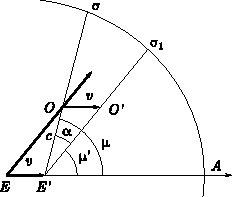
\includegraphics{figure/fig02.09}
    \caption{}
    \label{fig:02.09}
\end{wrapfigure}
\example 光行差现象。

具有不同运动状态的观察者所见的星体的方位是不同的,这
种差别叫做光行差。因地球公转运动而产生的光行差称为周年光
行差,因地球自转而产生的光行差称为周日光行差。

在图\ref{fig:02.09}~中,若观测者相对于某星是静止的,他观测到某星
在天球上的位置是$\sigma$,则星光到达望远镜物镜中心$O$时,其目镜位
置在$E'$点。若观测者跟随着地球运动,$EE'$为此时地球的运动方
向,因星光由$O$点到达目镜的时间为$\tau$,故在此时间内,地球运
行的距离为$EE'=\tau v$($\vec{v}$为地球运动的速度);因光速为$c$,当星
光到达目镜时,目镜已移至$E'$点,所以$OE'=\tau c$是星光在$\tau$内传
播的距离。若地球静止不动,则望远镜对准基的方向为$E'O$。当
地球运动时,望远镜指向$E'O'$方向才能接收到星光,这是星的视
方位。相应的,星由真位置$\sigma$移至视位置$\sigma_1$,

设星的真方位与观测者速度$\vec{v}$间的交角为\erratanote{$\mu$}{原书作“$u$”,疑为“$\mu$”误作“$u$”。本节误处据此改正。},星的视方位与
$\vec{v}$的夹角为$\mu'$,则光行差为$\alpha$,且有
\begin{equation*}
    \alpha=\mu-\mu'
\end{equation*}
由三角形$OO'E'$,得
\begin{equation*}
    \frac{\sin\alpha}{\sin\mu'}=\frac{OO'}{OE'}=\frac{\tau v}{\tau c}=\frac{v}{c}
\end{equation*}

\begin{equation*}
    \sin\alpha=\frac{v}{c}\sin\mu'
\end{equation*}
因为$\alpha$很小,所以
\begin{align*}
    \alpha&\approx\frac{v}{c}\sin\mu'\text{弧度} \\
        &=\frac{v}{c}\sin\mu'\times\frac{180}{\pi}\times 60 \times 60 \text{秒} \\
        &=\frac{v}{c}\sin\mu'\times 206265\text{秒} \\
        &=k\sin\mu'\text{秒}
\end{align*}
其中$k$称为光行差常数。

已知地球公转速率为$v=29.770\text{公里/秒}$,光速$c=299,774
\text{公里/秒}$,所以周年光行差常数
\begin{equation*}
    k_\text{年}=\frac{29.770}{299,774}\times 206,265=20.48\text{秒}
\end{equation*}

已知地球半径$R=6,378\text{公里}$。地球自转一周的时间为$T=
86,164\text{秒}$。所以在纬度$\varphi$处的地面速度为
\begin{equation*}
    v_\varphi=\frac{2\pi R\cos\varphi}{T}=0.464\cos\varphi\text{公里/秒}
\end{equation*}
因此,周日光行差常数为
\begin{align*}
    k_\varphi&=\frac{0.464}{299,774}\times 206,265\times\cos\varphi\text{秒} \\
        &=0.32\cos\varphi\text{秒}
\end{align*}
\section{加速度的相对性}\label{sec:02.04}
    根据速度合成公式\eqref{eqn:02.03.06},如果在时刻$t$,质点对于$K$,$K'$
的速度分别为$\vec{v}(t)$及$\vec{v}'(t)$,而$K'$相对于$K$以$\vec{u}$作匀速运动,则有
\begin{equation}\label{eqn:02.04.01}
    \vec{v}'(t)=\vec{v}(t)-\vec{u}
\end{equation}
根据加速度的定义。质点相对K的加速度是
\begin{equation}\label{eqn:02.04.02}
    \vec{a}\equiv\frac{\diff \vec{v}}{\diff t}
\end{equation}
而相对于$K'$的加速度是
\begin{equation}\label{eqn:02.04.03}
    \vec{a}'\equiv\frac{\diff \vec{v}'}{\diff t}
\end{equation}
将式(2·4·1)对时间求导,得
\begin{equation}
    \frac{\diff \vec{v}'}{\diff t}=\frac{\diff \vec{v}}{\diff t}-\frac{\diff \vec{u}}{\diff t}
\end{equation}
因u是不随时间变化的,故$\dfrac{\diff \vec{u}}{\diff t}=0$,所以得
\begin{equation}\label{eqn:02.04.04}
    \vec{a}'=\vec{a}
\end{equation}
这个结果告诉我们,同一质点对于两个相互匀速运动的参考系的
加速度是一样的。换言之,质点的加速度对于相对匀速运动的所
有参考系,具有不变性。

最后指出,对于相对以非匀速运动的两个参考系,式\eqref{eqn:02.04.01}
不再成立。例如,若$K'$相对于$K$作匀加速运动。加速度为$\vec{a}_0$,则
$K'$相对于$K$的速度为$\vec{u}=\vec{a}_0t$,从而式\eqref{eqn:02.04.01}相应改为
\begin{equation*}
    \vec{v}'(t)=\vec{v}(t)-\vec{a}_0t
\end{equation*}
由此可以推得
\begin{equation}\label{eqn:02.04.05}
    \vec{a}'=\vec{a} - \vec{a}_0
\end{equation}
这表示对于相对以匀加速度$\vec{a}_0$运动的两个参考系,质点对$K$及$K'$
的加速度$\vec{a}$及$\vec{a'}$,二者之间满足矢量加法关系(式\eqref{eqn:02.04.05}).在这
种情况,加速度是没有不变性或绝对性的。

\section{伽利略变换}\label{sec:02.05}

我们可以把前两节的结果概括如下,对于任何一组相互作匀

\noindent 速运动的参考系而言,速度是相对的,即同一质点相对于不同参
考系有不同的速度;加速度是绝对的,即同一质点相对于不同参
考系的加速度是一样的。

这些结果是相当平凡的,由日常生活的经验也不难接受这些
结果,它们似乎很“浅显”。然而,物理学的特点之一,就是不
放过任何一个“浅显”的概念,总是力图找出这些“浅显”概念
的根基是什么。上两节的目的,正是要找出由式\eqref{eqn:02.02.06}所表达
的速度相对性,和由式\eqref{eqn:02.04.04}所表达的加速度绝对性的根基。

它们的根基就是参考系$K$与$K'$的时空度量之间的变换关系。
现在,我们较仔细地分析一下这个变换关系。

仍假定$K$与$K'$二者相对作匀速运动,$K$的时空坐标为$t$,$\vec{r}$;$K'$
的为$t'$,$\vec{r}'$。$K$与$K'$的时空坐标之间的关系之一,由式\eqref{eqn:02.03.03}给
出,即
\begin{equation}\label{eqn:02.05.01}
    \vec{r}'=\vec{r}-\vec{u} t -\vec{d}_0
\end{equation}
其中$\vec{u}$是$K'$相对于$K$的运动速度。
在推导式\eqref{eqn:02.03.06}或式\eqref{eqn:02.04.04}时,我们还隐含地应用过另外
一个关系。注意在式\eqref{eqn:02.03.05}中我们用了
\begin{equation}\label{eqn:02.05.02}
    \vec{v}'=\frac{\dif \vec{r}'}{\dif t}
\end{equation}
它作为质点相对于$K'$的速度,然而,严格地说,$\vec{v}'$应定义为
\begin{equation}\label{eqn:02.05.03}
    \vec{v}'=\frac{\dif \vec{r}'}{\dif t'}
\end{equation}
即必须用$K'$系的时间$t'$。这样,对比式\eqref{eqn:02.05.02}及式\eqref{eqn:02.05.03}就可
以看到,在这里我们实质上假定$\dif t'=\dif t$,或者
\begin{equation}\label{eqn:02.05.04}
    t'=t+t_0
\end{equation}
其中,$t_0$为一常数。

式\eqref{eqn:02.05.01}及式\eqref{eqn:02.05.04}给出了$K$与$K'$的时空坐标之间的完整
的变换关系,它被称为伽利略变换。式\eqref{eqn:02.03.06}及式\eqref{eqn:02.04.04}都只
\clearpage
\noindent 是伽利略变换的推论。

伽利略变换表明,时间、空间具有下列的基本性质。

\heiti 1. 时间间隔的绝对性 \normalfont

对于一个运动过程,相对于$K$,它的开始与终了的时刻若分
别为$t_1$,$t_2$,则相对于$K'$它的开始与终了的时刻分别为$t_1'=t_1+t_0$,
$t_2'=t_2+t_0$,因此有
\begin{equation}\label{eqn:02.05.05}
    \Delta t \equiv t_2 - t_1 = t_2' - t_1' \equiv \Delta t'
\end{equation}
上式的物理意义是,一个过程的时间间隔与参考系的选取无关,
是绝对的。

\heiti 2. 长度的绝对性 \normalfont

有任一直尺,相对于$K$,它的两个端点的坐标为$\vec{r}_1$,$\vec{r}_2$,则相
对于$K'$,端点的坐标应分别是$\vec{r}_1' = \vec{r}_1 - \vec{u} t - \vec{d}_0$,$\vec{r}_2' = \vec{r}_2 - \vec{u} t - \vec{d}_0$,
故有
\begin{equation}\label{eqn:02.05.06}
    |\vec{r}_1 - \vec{r}_2| = |\vec{r}'_1 - \vec{r}'_2|
\end{equation}
它的物理意义是,一直尺的长度是与参考系的选取无关的,是绝
对的。

总之,速度相对性是以时间间隔和长度的绝对性为基础的,

\section{速度合成律的失效}\label{sec:02.06}

如图\ref{fig:02.10}~所示,如果在炮车上装有两门相同的大炮,一门向
右,一门向左。如果炮车相对地面静止〔图\ref{fig:02.10a}〕,这时,不论
从地面参考系$K$,还是从炮车参考系$K'$看,同时向左、右发射出
的炮弹的速率都是$v$。如果炮车相对地面以$u$的速率向右匀速运动
〔图\ref{fig:02.10b}〕,从$K$看,按速度合成规律〔式\eqref{eqn:02.03.06}〕,向右的炮
弹速率是$v+u$;向左的炮弹速率是$v-u$。实验也相当精确地证
明了这一点,它表明,速度的合成公式是符合实际的。

我们现在要问:速度合成律对任何情况都成立吗?

\clearpage
\begin{figure}
    \centering
    \subfigure[]{
        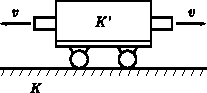
\includegraphics{figure/fig02.10a}
        \label{fig:02.10a}
    }
    \hspace{2em}
    \subfigure[]{
        \centering
        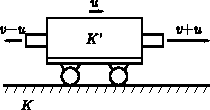
\includegraphics{figure/fig02.10b}
        \label{fig:02.10b}
    }
    \caption{速度的合成}
    \label{fig:02.10}
\end{figure}

\begin{figure}
    \centering
    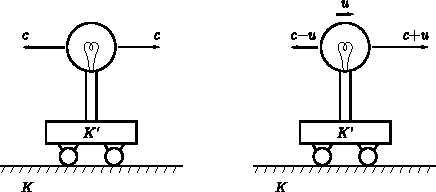
\includegraphics{figure/fig02.11}
    \caption{光的速度合成}
    \label{fig:02.11}
\end{figure}

再考虑一个如图\ref{fig:02.11}~所示的实验,这里仅把大炮改为灯泡,
灯泡发出的光与炮弹相当,光相对于灯泡的速率是$c$。根据速度合
成律,当灯泡相对于地面以速率$u$向右匀速运动时,则向右发出的
光对于地面参考系$K$的速率应是$c+u$,而向左发出的光对于$K$的
速率应是$c-u$。这个结果对吗?现在我们举一些显而易见的例
子,来说明这个结果是不正确的。

上述实验是把速度合成律应用到光传播的现象中去。根据光
学知识,我们知道,一个物体$A$之所以能被看到,是由于从物体
$A$发出的光(或从它反射的光)传到了我们的眼睛。例如,在图\ref{fig:02.12}~
中,1投球,2接球。2看到球$A$,是由于球$A$发出的光到达2。如果
光速为$c$,1到2之间距离为$L$,并且1即将投球的时刻为$t=0$,则
2看到1即将投球的时刻为
\begin{equation*}
    t_{2\text{投}}=\frac{L}{c}
\end{equation*}
\begin{figure}
    \centering
    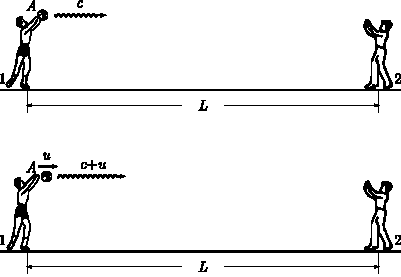
\includegraphics{figure/fig02.12}
    \caption{光的速度合成引起的混乱}
    \label{fig:02.12}
\end{figure}%
当1刚刚将球投出时,球$A$速率为$u$,如果光也满足速度合成律,
那么,这时球$A$发出的光相对于地面的速度应为$c+u$。如果1刚
刚将球投出的时刻是$t=t_{1\text{出}}$(即1投球这一动作所用的时间间隔),
则2看到1刚刚将球投出的时刻应为
\begin{equation*}
    t_{2\text{出}} = t_{1\text{出}} + \frac{L}{c+u}
\end{equation*}

从原则上讲。我们总有办法(譬如增大$L$)使下式成立
\begin{equation*}
    \frac{L}{c} > t_{1\text{出}} + \frac{L}{c+u}
\end{equation*}
亦即\vspace{-1.56em}
\begin{equation*}
    t_{2\text{投}} > t_{2\text{出}}
\end{equation*}
上式表明,2看到1开始投球的时刻比他看到1已经投出球的时刻
还要晚。更形象地说。2将先看到球$A$飞出,而后才看到1的投球
动作。这就是说,如果光的传播也满足速度合成公式\eqref{eqn:02.03.06},必然
导致先看到后发生的事,后看到先发生的事这种奇怪的现象,然
而,谁也没有见过这种现象。这说明光并不满足速度合成公式。

当然,有人会说,上述例子是假想实验,由于光速是很大
的,$L/c$或$L/(c+u)$实际上都接近于零,因而不可能观测到这种
现象。的确,在日常生活中涉及的速度与光速相比都是很小的,
把光速看成无限大,上述矛盾就没有了。但是,光速并不总能被
看成无限大,特别是在天体尺度上,光速不能被认为是无限大,光
传播中的矛盾是逃避不掉的。下面我们分析一个天文学上的真实
例子。

我国史书《宋史》中有下列的记载:“至和元年五月己丑出
天关东南可数寸岁余稍没”,《宋会要辑稿》也记载:“至和元
年五月晨出东方守天关昼见如太白芒角四出色赤白凡见二十三
日”。这个重要的天文观测记录说的是一次非常著名的超新星爆
发事件,现称为公元1054年的超新星。

所谓超新星指的是恒星在特定的演化阶段出现的一次大爆
发。原来发光很弱的星体,在爆发时,向外抛出速率很高的大量
物质,并发出很强的光,过不长的一段时间,又再暗下去。现在
巳确定,1054年超新星的遗迹就是金牛座中的蟹状星云,它到地
球的距离约为$L \approx 5000$光年,爆发时,喷射物的速率至少有
$u=1500$公里/秒。
\begin{figurex}
    \centering
    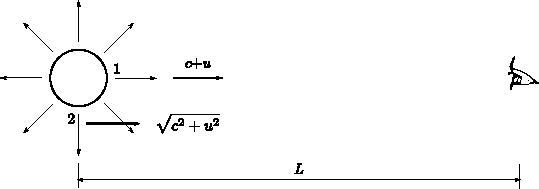
\includegraphics{figure/fig02.13}
    \caption{超新星爆发过程中光的传播}
    \label{fig:02.13}
\end{figurex}

由图\ref{fig:02.13}~看出,如果爆发时刻为$t=0$,且爆发时间极短,则
根据速度合成律,1处发出的传向观察者的光相对地面的速率是
$c+u$,所以观察者看到l发光的时刻是

\begin{equation*}
    t_{1}=\frac{L}{c+u} \approx \frac{L}{c}\left(1-\frac{u}{c}\right)
\end{equation*}
同样,根据速度合成律,2处(弧$\overset{\frown}{12}=\ang{90;;}$)发出的传向观察者的光
相对于地面的速率约为$\sqrt{c^2 + u^2}$,故观察者看到2发光的时刻是
\begin{equation*}
    t_{2}=\frac{L}{\sqrt{c^{2}+u^{2}}} \approx \frac{L}{c}\left(1-\frac{1}{2} \cdot \frac{u^{2}}{c^{2}}\right)
\end{equation*}
显然,观察者见弧$\overset{\frown}{12}$中发光的时刻介于$t_1$到$t_2$之间,因此观察者
看到星发光的时间至少应是
\begin{equation*}
    \Delta t=t_{2}-t_{1} \approx \frac{Lu}{c^{2}}
\end{equation*}
代入有关数据,计算而得
\begin{equation*}
    \Delta t=25\text{年}
\end{equation*}
如果爆发不作瞬时过程处理,则看到超新星的时间应比25年
还要长。

但是,这个下限与实际观测是不相符合的。记录上说:“凡
见二十三日”(白天看到)或“岁余稍没”(夜里看到)。即一年多
就消没了。

上述真实例子说明,对于光传播的现象,速度合成律是失效
的。它说明,从超新星不同地方发出的光,即不同光源发出的光,
相对于地面的速率之闻的差别,不应有式\eqref{eqn:02.03.06}~所给出的那样
大。现代更精确的实验表明。光速是与光源速度无关的,无论光
源的速度有多么大,由它发出的光的速度仍与静止光源发出的光
的速度相同。这就是光速不变性,这个特点最初是由爱因斯坦注
意到的。

显然,光速不变性与速度合成律〔式\eqref{eqn:02.03.06}〕之间存在着严重
的矛盾,而问题的根源就在于伽利略变换并不总是适用的。
\section{光速不变的结论之一——运动钟的变慢}\label{sec:02.07}

现在我们来分析,从光速不变性能得出什么结论。光速不变
性使我们所看到的物理现象总是因果相继的,免除了因果倒置的
混乱。但是,光速不变性却动摇了另一个传统观念一时间间隔
的不变性。

我们可以用光速不变性来设计一种雷达钟。图\ref{fig:02.14a}~是一
个雷达式的装置,在距离雷达天线$d$处放一反射镜,那么,从天
线发出光信号到天线重又接收到这个光信号一个来回的时间间隔
应为
\begin{equation*}
    \Delta t ' = \frac { 2 d } { c }
\end{equation*}
\begin{figure}[!h]
    \centering
    \subfigure[]{
        \label{fig:02.14a}
        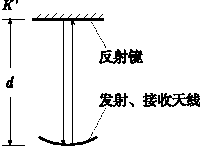
\includegraphics{figure/fig02.14a}
    }
    \quad
    \subfigure[]{
        \label{fig:02.14b}
        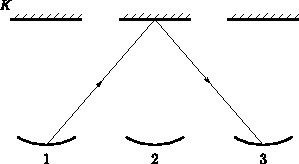
\includegraphics{figure/fig02.14b}
    }
    \caption{雷达钟}
    \label{fig:02.14}
\end{figure}

由于光速不变,我们可以用一个来回作为度量时间的单位。这个
装置就是一种钟。

现在,我们让这个钟固定在$K'$中,一起以匀速$u$相对于K沿
垂直于$d$的方向运动。在$K'$中看,光信号一个来回仍走$2d$,它的
时间间隔仍为
\begin{equation*}
    \Delta t ' = \frac { 2 d } { c }
\end{equation*}
% 079.jpg
但是在$K$中看来,光信号这时走的是之字形路径〔图\ref{fig:02.14b}〕光
信号发出时,钟位于1,镜反射光信号时,位于2,接收光信号时,
位于3。因而,这光信号的一个来回,在$K$中看来是走两条斜线。
如果这个来回在$K$中看,所需时间间隔为$\Delta t$,则按光速不变性,
斜边长为$\dfrac { 1 } { 2 } c \Delta t $ ,底边1到2的长$\frac { 1 } { 2 } u \Delta t$  ,故由直角三角形关系
有
\begin{align*}
    \left( \frac { 1 } { 2 } c \Delta t \right) ^ { 2 } &= \left( \frac { 1 } { 2 } u \Delta t \right) ^ { 2 } + d ^ { 2 } \\
&= \left( \frac { 1 } { 2 } u \Delta t \right) ^ { 2 } + \left( \frac { 1 } { 2 } c \Delta t ' \right) ^ { 2 }
\end{align*}
解之得
\begin{equation}\label{eqn:02.07.01}
    \Delta t = \dfrac { \Delta t ' } { \sqrt { 1 - \dfrac { u ^ 2 } { c ^ { 2 } } } }
\end{equation}
此式表明,在$K'$中需用$\Delta t '$时间间隔的过程,在$K$中观测就
不等于$\Delta t$,而是$\Delta t > \Delta t '$ 。当$K'$中的钟走了一个单位时间间隔
即$ \Delta t ' = 1  $时,$K$中的钟已走了
$\dfrac { 1 } { \sqrt { 1 - \dfrac { u ^ 2 } { c ^ { 2 } } } } > 1$。也就是说,由$K$看
来,$K'$中的钟变慢了。$K$看$K'$的钟是在运动,故运动的钟变慢。
反过来,由$K'$来看$K$中的钟时,我们可以用完全相同的推理
方法(注意此时$K$沿$K'$的$x'$的负向以速率作匀速运动),得到
\begin{equation}\label{eqn:02.07.02}
    \Delta t ' = \dfrac { \Delta t } { \sqrt { 1 - \dfrac { u ^ 2 } { c ^ { 2 } } } }
\end{equation}
可见,$K'$看$K$中的钟也变慢。

有人会说,这岂不矛盾!其实并不矛盾。因为他们是在不同
的“立场”上说话的,两种说法实际上是一致的,可以统一地表
% 080.jpg
达为:相对于观测者运动的钟变慢。

时间的变慢已有大量的实验证明。最有名的是$\mu$子的衰变。
从实验室中产生的$\mu$子,寿命只有约~$\num{2.2e-6}$~秒,这样,即使它
以光速$ c \approx \num{3e8} $米/秒运动,也只能走过\vspace{-0.2em}
\begin{equation*}
    \num{2.2 e -6} \times \num{3e8} = 660 \text{米}
\end{equation*}

\vspace{-0.2em}另一方面,宇宙射线产生子的区域约在1500$\sim$2000米的高
空。但是我们发现不少从上层大气中产生的从子跑到地面上来了。
为什么?就因为寿命~\num{2.2 e -6}~秒是对于$\mu$子静止的参考系$K'$而
言的,当$\mu$子运动时,在地面上(即参考系$K$)看来,它的寿命应为
$\Delta t = \dfrac { \num{2.2e-6}}{ \sqrt { 1 - \dfrac { u ^ 2 } { c ^ { 2 } } } }$
秒,其中$u$是$\mu$子的运动速度,当$u$接近于$c$
时,$\Delta t$比~\num{2.2e-6}~秒大得多,即$\mu$子的寿命变长了,因而它可以
飞过距离
\begin{equation*}
    L = u \Delta t \gg 660 \text{米}
\end{equation*}
即能从高空飞到地面上来。

1964年,欧洲核子研究中心(CERN)通过实验定量地验证了
时间延长公式。用两个同时产生的$\mu$子,让其中之一相对于实验室
静止,另一个在加速器中运动。结果证明,运动子的寿命变长,
两子的寿命比值和在加速器中的运动速度$u$之间的关系完全符合
式\eqref{eqn:02.07.02}。

运动钟变慢与我们从日常生活中得来的感觉完全不同。因此,
不免有人会问:“到底钟是否真的变慢了?”物理学,特别是力
学,有很多内容是描写我们日常看到和感觉到的东西的。但是,
物理学与我们日常的直观有很多不同。物理学要求每个陈述有明
确的含义,特别是要指出每一个物理量是如何测量的,然后再在
这个基础上研究规律的建立。一般地诉诸于感觉如何如何,这不
是物理学,只不过是粗浅的认识。
% 081.jpg

上述的“到底”一问似乎很有道理,但却是没有物理价值的,
为什么?因为该处的“到底”是不能测量的。如果能指出“到底”
是在什么情况下进行什么测量的,我们才可作出明确的回答。如
果不能指出这一点,那说明这个问题本身就是非物理的,物理学
不研究这类问题。一旦研究测量方法,而测量又要相对于一定的
参考系,则必然走到我们上述的体系中去。

物理学的基础是测量,如果在原则上含有不能测量的东西,
这种东西本身就缺乏物理意义,因为这种不能测量的东西,既无
法用实验证实它,也无法否证它。用现代物理学的语言说,一种
理论要具有物理价值,就要具有可证伪性,即所有有关的量以及
断言,都能直接或间接由实验加以验证。这是我们判断一种理论
有没有物理价值的基本原则之一。
\section{光速不变的结论之二——运动尺的变短}\label{sec:02.08}

在上节中,我们看到光速不变动摇了伽利略变换的根基之
一—时间间隔的绝对性。现在我们将证明,在光速不变的前提
下,伽利略变换的另一个根基一长度的绝对性也不再成立。

对地面上的观测者来说,从大气层上部冲下来的μ子的寿命
延长了。随同μ子一起运动的观测者会看到什么情况呢?

由于相对于子为静止的观测者与地面上的观测者都同样观
测到从子从高空运动到地面这一事实,而且他们也都观测到他
们之间的相对速度是$u$。对于地面上的观测者来说$\mu$子的寿命$\Delta t = \dfrac{\num{2.2e-6}}{\sqrt{1 - \dfrac{u ^ 2}{c ^ 2}}}$
秒,$\Delta t$大了,故$ L ( = u \Delta t )$大于$\mu$子出生处到地面的
高度,所以它能到达地面。而随$\mu$子运动的观察者所看到$\mu$子的寿
命应是~\num{2.2e-6}~秒。那么他怎么解释$\mu$子到达地面这一事实呢?
% 082.jpg
这只能有一种可能性,即随同$\mu$子运动的观测者主张:$\mu$子出生
处到地面的距离变短了。即一旦时间间隔不变性不成立,则长度
不变性也要被破坏。如果我们设想从地面到高空立着一个尺,尺
静止在地面上,地面观察者看尺长为$L$;而相对于$\mu$子静止的观
察者看来,这尺长为$L'$,即
\begin{equation*}
    \frac { L } { \Delta t } = \frac { L ' } { \Delta t ' }
\end{equation*}
\begin{equation}\label{eqn:02.08.01}
    L ' = L \frac { \Delta t ' } { \Delta t } = L \sqrt { 1 - \frac { u ^ { 2 } }  { c ^ { 2 } } }
\end{equation}
这尺对于$\mu$子上的观察者在运动,故$ L ' < L  $,即运动的尺变短。

\begin{figurex}[!b]
    \centering
    \subfigure[静止的雷达钟]{
        \label{fig:02.15a}
        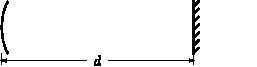
\includegraphics{figure/fig02.15a}
    } \\ \vspace{-0.3em}
    \subfigure[运动的雷达钟]{
        \label{fig:02.15b}
        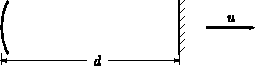
\includegraphics{figure/fig02.15b}
    } \\ \vspace{-0.3em}
    \subfigure[光信号向右传播]{
        \label{fig:02.15c}
        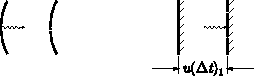
\includegraphics{figure/fig02.15c}
    } \\ \vspace{-0.3em}
    \subfigure[光信号向左传播]{
        \label{fig:02.15d}
        \includegraphics{figure/fig02.15d}
    }
    \caption{}
    \label{fig:02.15}
\end{figurex}
现在我们来证明式\eqref{eqn:02.08.01}。我们仍使用一个雷达钟。如
图\ref{fig:02.15a}~所示,当雷达钟与地面相对静止时,从地面参考系,即$K$
% 083.jpg
系来观察,它的天线与反射面之间的距离为$ d$;当雷达钟以速度
运动时\lhbrak 图\ref{fig:02.15b}\,\rhbrak ,由$K$系测得的距离表示为$d'$。

我们考察光信号来回一次的运动。由于光在传播过程中雷达
在不断地运动,所以,由$K$看来,光传播的距离并不是$d'$。例如,
当光向右传播,从天线到达反射面时,若所用的时间为$(\Delta t)_1$,则
所走过的距离应为$ d ' + u ( \Delta t ) _ { 1 }$,其中\erratanote{$ u ( \Delta t) _ { 1 } $}{原书作“$ u ( \Delta t _ { 1 })$”,联系上下文,显误。}一项表示在$(\Delta t)_1$时
间中钟向右运动的距离\lhbrak 图\ref{fig:02.15c}\,\rhbrak 。这样,我们有
\begin{equation*}
    ( \Delta t ) _ { 1 } = \frac { d ' + u (\Delta t)_1 } { c }
\end{equation*}
或者
\begin{equation}\label{eqn:02.08.02}
    ( \Delta t ) _ { 1 } = \frac { d ' } { c - u }
\end{equation}
类似地,光从反射面到天线的传播过程所用的时间(Δt)2应是
\begin{equation}\label{eqn:02.08.03}
    ( \Delta t ) _ { 2 } = \frac { d ' } { c + u }
\end{equation}
由式\eqref{eqn:02.08.02}及式\eqref{eqn:02.08.03}可以得到光信号一个来回耗费的时间
\begin{equation}\label{eqn:02.08.04}
    \Delta t = ( \Delta t ) _ { 1 } + ( \Delta t ) _ { 2 } =  \frac { 2 c d ' } { c ^ { 2 } - u ^ { 2 } }
\end{equation}
这是$K$系看到的结果。

在$K'$系,即雷达钟参考系来看,这个过程仍由下式描写
\begin{equation*}
    ( \Delta t ) ' = \frac { 2 d } { c }
\end{equation*}
因为在$K'$系观察,钟的长度是$d$。这样,式\eqref{eqn:02.08.04}可以改写为
\begin{equation*}
    \Delta t = \frac { 1 } { 1 - \dfrac { u ^ { 2 } } { c ^ { 2 } } } \left ( \frac { d ' } { d } \right) \left( \Delta t \right) '
\end{equation*}
再由上节推知的时间关系式\eqref{eqn:02.07.01},上式就成为
\begin{equation*}
    d ' = d \sqrt { 1 - \frac { u ^ { 2 } } { c ^ { 2 } } }
\end{equation*}
% 084.jpg
\clearpage
\noindent 这就是式\eqref{eqn:02.08.01}

本节和上节的讨论用的都是雷达钟,因此,就存在一个共同
的问题,即运动钟的变慢和运动尺的变短是否普遍?或者,这些
推论是否只反映了雷达钟本身的性质,如果选择其他的钟有没有
这种性质?这些问题我们留待第十一章再来讨论

\questions

\question 在亚里士多德体系中,哪些物理量是绝对的?哪些物理量
是相对的?在牛顿体系中,哪些物理量是绝对的?哪些物理量是
相对的?

\question 变换关系式\eqref{eqn:02.03.06}是否只适用于$u$为常量的两个坐标间
的速度变换?

\question 试再举出一些有用的坐标变换。

\question 试举出一种相对于时间倒转变换为不变的运动。

\begin{wrapfigure}[10]{r}{12em}
    \includegraphics{figure/fig02.16}
    \caption{}
    \label{fig:02.16}
\end{wrapfigure}

\question 双星是一种天体,两颗星
绕它们共同的质心在一封闭的轨
道上绕行(图\ref{fig:02.16}),如果我们的
视线在轨道平面上,则双星中任
何一颗星有时向着我们运动,有
时离开我们运动。假使光速与光
源速度有关,可用速度合成公式
\eqref{eqn:02.03.06}。这样,我们将会看到什
么现象?

\question 如果地球总是以恒定的
速度运动,也没有自转,能探测到光行差效应吗?

\question 由于地球的周年运动引起的光行差效应,使得恒星的视位
置在一年之中绘出怎样的图形?
% 085.jpg
\clearpage
\question 在\ref{sec:02.07}~节中所述“运动钟的变慢”,是否是由于我们选用的雷达钟的特殊结构而引起的?
\exercises
\fangsong

\exercise 以不同的速率同时向不同方向抛出两物体。证明在运动的
时候,若不计空气阻力,它们的相对速度固定不变。

\exercise 有一水平飞行的飞机,速度为$ v _ { 0 }$,在飞机上安置一门炮,炮弹以水平速度v向前射击。略去空气阻力,求

(1) 以地球为参考系时炮弹的轨迹

(2) 以飞机为参考系时炮弹的轨迹

(3) 以炮弹为参考系时飞机的轨迹

\exercise 一辆汽车尾部敞开,顶篷只盖到$A$处(图\ref{fig:02.17}),乘客可坐
\begin{wrapfigure}[7]{r}{12em}
    \includegraphics{figure/fig02.17}
    \caption{}
    \label{fig:02.17}
\end{wrapfigure}
到车尾$B$处,$AB$联线与铅直方向
成$ \varphi = 3 0 ^ { \circ }  $角。汽车在平直公路上
冒雨行驶,当其速率为6公里/时
时,$C$点刚好不被雨打着若它
的速率为18公里/时,则$B$点就
刚好不被雨点打着。求雨点的速
度$ v _ { 0 }$

\exercise 以速率$ v _ { 1 }  $运动的列车上的驾驶员,发现在前面与该车相距
$d$处,有一列车在同一轨道上沿相同方向、以较小的速率$v_2$在运
动,他立刻用制动器刹车,使他的火车以匀减速$a$慢下来,试证
明:

(1) 如果$d > \dfrac { ( v _ { 1 } - v _ { 2 } ) ^ { 2 } } { 2 a }$
则两车不会相撞;

(2) 如果$d < \dfrac { ( v _ { 1 } - v _ { 2 } ) ^ { 2 } } { 2 a }$
,则两车将要相撞。
% 086.jpg

\exercise 渔人在河中乘舟逆流航行,经过某桥下时,一只水桶落入
水中,半小时后他才发觉,即回头追赶,在桥的下游5.0公里处赶
上。设渔人顺流及逆流相对水的划行速率不变,求水流速率。

\exercise 甲乙两列火车在相邻的轨道上相向运行,甲的速率为$v_1$,
乙的速率为$v_2$。从甲车上水平地投一物到乙车上。设投掷速率为
$v _ { 0 }$ ( $v_0  $在物体运动的全部时间内可认为是不变的),从甲车上看,投
掷方向与列车行驶方向垂直,试求:

(1)物体的轨迹在路基上的投影与铁轨所成的角φ13

(2)物体的轨迹在乙车上的投影与乙车边缘所成的角甲23

(3)物体相对于路基的速度v和相对于乙车的速度v。

\exercise 飞机的罗盘指示飞机正在朝东飞行,地面上的情报指出,
此时刮着正南风。如果风速$ | \vec{u} | = 4 0 . 0  $公里/时,飞机相对空气的
速度为$ | \vec{v} ' | = 2 0 0  $公里/时,试用矢量图表明:飞机相对于地面的
速度$\vec{v}$;驾驶员应怎样驾驶才使其前进方向相对于地面是朝向正
东?

\exercise 一架飞机以相对于空气的匀速率$u$作水平直线飞行,从$A$飞
到$B$再返回,从$A$到$B$的距离是$L$。如果速率为$v$的风向有下列三
种情况(都有$ u > v$)  :

(1)沿着从$A$到$B$的直线

(2)垂直于从$A$到$B$的直线

(3)与$A$到$B$的直线成角。\\
试求往返一次所需要的时间。并证明,由于风的存在,往返时间
总是比无风的情况长。

\exercise 一升降机以$ a = 2 g  $的加速度从静止开始上升,在2.0秒末时
有一小钉从顶板下落,若升降机顶板到底板的距离$ k = 2 . 0  $米,求
钉子从顶板落到底板的时间$t$,它与参考系的选取有无关系?

\exercise 一飞机在海上布雷,当它在水面上高为$h$的地方以速率$v$
沿水平方向飞行时,要想使鱼雷入水时,鱼雷不与水面发生拍击,
% 087.jpg
\begin{wrapfigure}[8]{r}{15em}
    \includegraphics{figure/fig02.18}
    \caption{}
    \label{fig:02.18}
\end{wrapfigure}
即相对于鱼来说,水的速度完全沿鱼雷的轴线方向
(图\ref{fig:02.18})。设鱼雷从投下到入水,它的轴线与水平面的
夹角不变。略去空气阻力,求当飞机投射鱼雷时,$\theta$应
当等于多少?

\exercise 设某一超新星到地
球的距离$ L \geqslant 1 0 ^ { 6 }  $光年,若爆发是匀速球状膨胀,膨胀速率$|\vec{v}|$约为$5 \times 1 0 ^ { - 3 }  $光年/年。如果光速与光源速度有关,爆发后,在地球上
有多长时间间隔都能观测到它的最大光度?

\exercise 在某一参考系$K$看来,物体$A$以匀速率$v_A$沿$x$轴正向运动,
物体$B$以匀速率$v_B$沿$x$轴的负方向运动。试问:

(1) 在参考系\*$K$\*看来,\!$A$\*与\*$B$\*之间相对运动的速度\*$v_{A\!B}$\*是多大?

(2) $c$\*为真空中的光速,当\*$ v _ { A }$=0.8$ c $,\!$ v _ { B }$=\*0.6$ c  $\,时,\!$v_{A\!B}$\*是多少?

(3) 在同一参考系$K$中看来,两个物体$A$与$B$之间相对运动的
速度$ v _ { A B } > c  $,是否违反狭义相对论?为什么?

(4) 在$A$看来(即在随$A$一起运动的坐标系$K'$里看),$B$的速
度$ v _ B ' $仍旧是$v_{AB}$吗?

\exercise~ $K$和$K'$是两个相互平行的系,$K'$相对于$K$沿$x$轴以的$\dfrac { 1 } { 2 } c $速率运动。问:

(1) 在$K$系中静止放置一把尺子,长为$l$,在$K'$系来测量,尺
子的长度是多少?

(2) 在$K$系中某点$A$发生一事件,时间间隔为$\Delta t$,在$K'$系来
看,这事件的时间间隔是多少?

\exercise 在实验室中观测到一个运动着的$\mu$子在实验室坐标系中
的寿命等于静止$\mu$子寿命的50倍,求$\mu$子相对于实验室坐标系
\clearpage

\noindent 运动
% 088.jpg
的速度$v$。

\exercise 爱因斯坦在他的创立狭义相对论的论文中说:“一只在
地球赤道上的钟,比放在两极的一只在性能上完全一样的钟,在
别的条件都相同的情况下,要走得慢些。”根据各种观测,地球
从形成到现在约为50亿年。假定地球形成时,就有爱因斯坦所说
的那两只钟,问:现在它们所指示的时间相差多少?已知地球半
径为6378公里。\vspace{-0.14em}

\exercise 按上题同样道理,在地球看来,一只在月球上的钟,要比
一个性质完全相同,所处条件也完全相同,放在地球上的钟走得
略为慢些。设地球年龄为$ \tau = 5 0  $亿年,月球绕地球转动的平均速率
为$ v = 1 . 0 2 \times 1 0 ^ { 5 }  $厘米/秒。月球上的钟在50亿年里比地球上的钟慢了多少?\vspace{-0.14em}

\exercise 类似15题,在太阳上的观测者将看到一只在地球上的钟,
要比一只性能完全相同、所处条件也完全相同放在太阳上的钟走
得略为慢些。设太阳年龄为$ \tau = 5 0  $亿年,已知地球公转的平均速率
为$ v = 2 9 . 7 6  $公里/秒。地球上的钟在50亿年里比太阳上的钟慢了
多少?\vspace{-0.14em}

\exercise 一个“光钟”由两个相距为$ L _ { 0 }  $的平面镜$A$和$B$组成。对于
这个光钟为静止的参考系来说,一个“滴答”的时间是光从镜面
$A$到镜面$B$再回到原处的时间,其值是$ t _ { 0 } = 2 L _ { 0 }  /c$。若将这个光钟横
放在一个以速度$\vec{v}$行驶的火车上,使两镜面都与$\vec{v}$垂直,而两镜
面中心联线则与$\vec{v}$平行。这时,若在铁轨参考系中看,火车上钟
的一个“滴答”$\tau$与$\tau _ 0$的关系怎样?\vspace{-0.14em}

\exercise ~ $\mu$子是不稳定的粒子,它自发地衰变为 \vspace{-0.2em} \\
\null\hspace{6em} $\mu ^ \pm \longrightarrow e ^ \pm + \overline{\nu} _ { e } + \nu _ { \mu }$ \vspace{-0.2em} \\
{\ziju{-0.01}其中\*$\mu ^ \pm$\*分别表示带正电或带负电的\*$\mu$\*子,\!$\overline{\nu} _ { e }$\*表示反中微子,\!$\nu _ { \mu}$\*表示$\mu$\*中微子。上述自发衰变的寿命是\*$ \tau _ { 0 }$=2.2$\times$10$^{-6}$\*秒,这是对\*$\mu$\*子静
止的坐标系而言的。\!若\*$\mu$\*子的速度\*$ v$=0.995$c$,\!它的寿命将为多少?}
\normalfont

% 第三章
\chapter{牛顿动力学}\label{chp:03}
\section{惯性定律}\label{sec:03.01}

在上两章中,讨论了运动的描述,而没有涉及运动的原因,
没有研究不同式样的运动之间的内在联系。譬如,自由落体为什
么垂直向下做匀加速运动?行星为什么绕太阳旋转不息?自由落
体与行星旋转两者之间有什么关系?这些就是本章及随后几章要
讨论的问题。

研究物体运动的原因,通常称之为动力学。牛顿动力学就是
有关物体的机械运动的动力学。可以说整个物理学的基本规律就
是各种运动形态的动力学的总合。

牛顿动力学中的核心概念是力。

经验告诉我们,物体的运动是由物体之间的相互作用引起的。
列车的行进是由于机车的牵引作用,枪弹的射击是靠着炸药爆炸
的作用。物体之间的相互作用,用“力”这个概念来表达。实际
上,人对力最初的认识是源于人的肌肉对外物的作用。汉字的力,
在篆书中的写法,就是筋肉的象形。

力的概念虽然出现得很早,但是关于力和运动的关系的正确
认识,却得到得相当晚。在亚里士多德的《物理学》中有一条原
理:“凡运动着的事物必然都有推动者在推动着它运动。”这个
论断在几乎两千年的时间里,被认为是无可怀疑的经典。的确,
% 090.jpg
我们日常看到的各种运动似乎都遵从这个论断,即必定有推动者
(即力)在维持着它的运动。就象一定的踏力保持着自行车的一定
的运动状态,而一当踏力消失,车最终要变成静止。

\begin{wrapfigure}[7]{r}{16em}
    \includegraphics{figure/fig03.01}
    \caption{伽利略的斜面}
    \label{fig:03.01}
\end{wrapfigure}
伽利略开始明确地认识到亚里士多德的经典是不完全正确的,尽
管许多运动的确都要靠外力的维持,但并非凡运动皆如此。伽利略用
一个理想实验来证明亚里士多德的错误。他研究斜面上的运动(图\ref{fig:03.01}),
让一小球从斜面
上滚下。已经知道,小球的下滚是由于重力的作用,重力沿着斜面
的分量拉着小球下滚。如果高度不变,$\alpha$越小,则L越大,同时
重力沿斜面的分量也越小。伽利略曾做过一系列小球沿斜面下滑
的实验。他发现,只要斜面足够光滑,无论$\alpha$多么小,小球总能
从斜面上滚下来。由这个结果就可以推测,即使当$ a \rightarrow 0$  ,$L \rightarrow \infty$
的情况,小球还是可以滚“下”来的。显然,对$ a \rightarrow 0$  ,$L \rightarrow \infty$情
况是无法直接做实验的,但从已知的实验结果可以推知这种极限
情况的现象。这就是理想实验方法的关键。

在$ a \rightarrow 0$  ,$L \rightarrow \infty$情况,重力沿斜面的分量为零,即并没有外
力推动小球“下”滚。因此,这种运动就是一种没有“推动者”
的运动。对亚里士多德的“凡运动必有推动者”来说,上述运动
就是一个反例。

伽利略的分析弄清了,存在一类运动,它们并不是由外力所
维持。它们的特征是速度保持不变,即作匀速率的直线运动,或
者静止。我们称物体不受外力作用的运动状态为自由运动。总之,
处在自由运动状态的物体,必定作匀速直线运动,或者静止。这
就是惯性定律。
% 091.jpg

有人可能会想到,速度或加速度都是具有相对性的,对参考
系$K$为匀速运动的物体,在参考系$K'$中可能成为非匀速的。那么,
一个自由运动的物体,在有些参考系看来不也是作着非匀速运动
吗?的确,在某参考系看来,一个不受力的物体也会作非匀速运
动。

然而,惯性定律的意义是在于断言:对于一个物体的自由运
动,一定可以选择一个参考系$K$,相对于$K$该物体作匀速运动或
静止,而且,其他所有自由运动的物体,对于$K$来说,也都是作
匀速运动或静止。换言之,一定存在着这样的参考系,相对于
它,所有不受外力作用的物体都保持自己的速度。这类特殊的参
考系,称为惯性参考系,或惯性系。

简言之,惯性定律就是断定了惯性系一定存在。

惯性定律的确立,成为旧物理学(即亚里士多德物理学)的终
点,同时也成为新的力学的起点。常称惯性定律为牛顿第一定律。
本章以后的讨论,都采用惯性系。
\section{牛顿第二定律}\label{sec:03.02}

{\ziju{-0.01}牛顿第一定律确立了不受力情况下物体的运动性质。本节讨
论牛顿第二定律,它确立了外力对物体运动的作用。这个定律是:
如果一个质点受到外界物体的作用,则它的运动遵循下列关系:}
\begin{equation}\label{eqn:03.02.01}
    \vec{F} = m \vec{a}
\end{equation}
其中\,$\vec{a}$\,是质点的加速度,$m$\,是它的质量;$\vec{F}$\,是外物对它的作用力。

{\ziju{-0.01}在此定律中,我们一下子涉及了两个新的物理量:$m$及$\vec{F}$。虽然
在上节讨论过力,但只限于受力或不受力,并没有给出力的定量的
定义,以及如何从动力学的角度来定义力。另一方面,质量的粗浅
概念也早就有了,问题同样是:什么是质量?并未解决。也曾有过各
式各样的有关质量的定义。例如,有的定义是:质量是物体所含
% 092.jpg
“物质的量”然而,这种定义没有物理的价值。因为,什么叫“物质
的量”?仍然是不确定的。在物理学中,一个物理量的定义,必
须提供根据其他能够量度的量来计算它的一套规则。根据这个原
则,在牛顿第二定律的范围中,可以对质量及力作如下的定义:}

质量就是质点所受外力与所产生的加速度之比。

作用在一个质点上的力就是它的质量乘由于该力所产生的加
速度。

看到这两条“定义”,读者一定会纳闷,这两条说法岂不就
是式\eqref{eqn:03.02.01}的改头换面吗?这样一来,作为定律的式\eqref{eqn:03.02.01}岂
不降为关于质量或力的定义?似乎出现了逻辑上的“混乱”。

如果离开上述的物理定义的原则,确实总逃不脱这个“混
乱”。但是,从物理上来说,它是不混乱的。物理规律的作用在
于把许多已知的实验结果统一起来,联系起来,给出许多实验现
象的统一的解释,并且根据这种解释去预测一些新的现象或实验
结果。也就是说,物理学规律的意义,是使我们能够从一些实验结
果出发预言另一些新的实验结果,确立从一些实验数据计算出(或
预言出)另一些实验数据的规则。只要定义、定律确立的联系测
量数据的规则是明确的、不含糊的,那就没有任何“混乱”可
言。牛顿第二定律〔\eqref{eqn:03.02.01}〕及质量和力的定义在这种意义上是
没有任何“混乱”的。

举例说明。如图3.2所示,在一足够光滑的固定桌面上,我
\begin{figurex}[!h]
    \centering
    \hfill
    \subfigure[]{
        \label{fig:03.02a}
        \includegraphics{figure/fig03.02a}
    }
    \hfill
    \subfigure[]{
        \label{fig:03.02b}
        \includegraphics{figure/fig03.02b}
    }
    \hfill
    \subfigure[]{
        \label{fig:03.02c}
        \includegraphics{figure/fig03.02c}
    }
    \hfill
    \label{fig:03.02}
    \caption{牛顿第二定律的含义}
\end{figurex}
% 093.jpg
\clearpage
\noindent 们做三个实验。其一,物体$ A $与一弹簧相连,把弹簧拉长到$ L $,然后
释放物体$ A $,在弹簧的牵动下,$ A $作加速运动,测量出开始时刻的
加速度$ a_A $;其二,用上述弹簧与物体$ B $相连,仍拉长到$ L $,测出
释放时刻的加速度$  a _ { B  } $;  其三,仍是上述弹簧,拉长到$ L $,和捆在
一起的$ A $,$ B $相连,测出释放时刻的加速度$  a _ { A B }  $。

上述三个实验,只用了运动学的概念,测得了一组数据,如
果没有其他知识,我们就不能得到更多的东西。现在,我们看如
何用动力学来得到的测量量$ a_A $,$ a_B $,$ a_{AB} $之间的联系。

我们可以取物体$ A $的质量作为质量单位的标准,故可任意定
其数值为$ m_A $,利用式\eqref{eqn:03.02.01}作为力的定义,再由实验\subref{fig:03.02a}测得
的$ a $即可算出弹簧对$ A $的牵动力
\begin{equation}\label{eqn:03.02.02}
    F = m _ { A } a _ { A }
\end{equation}

在实验\subref{fig:03.02b}中,设弹簧对$ B $的牵动力与牵动$ A $时一样,仍为$ F $,
则利用式\eqref{eqn:03.02.01}作为质量的定义,可算出$ B $的质量
\begin{equation}\label{eqn:03.02.03}
    m _ { B } = \frac { F } { a _ { B } }
\end{equation}

在实验\subref{fig:03.02a}中,如果假设$ A $与$ B $在一起的质量$ m_{AB} $是分别质量
之和(即质量是可加的):
\begin{equation}\label{eqn:03.02.04}
    m _ { A B } = m _ { A } + m _ { B }
\end{equation}

再假定牵动力依然是F,就可以用式\eqref{eqn:03.02.01}作为定律,来预
言此时的加速度$ a_{AB} $为
\begin{equation}\label{eqn:03.02.05}
    a _ { A B } = \frac { F } { m _ { A B } } = \frac { F } { m _ { A } + m _ { B } } = \frac { a _ { A } a _ { B } } { a _ { B } + a _ { A } }
\end{equation}

{\ziju{-0.005}我们注意到,式\eqref{eqn:03.02.05}中只含有实验直接可测的量(与我们
任意取定$ m_A $值无关),亦即牛顿第二定律给出了从一组实验〔\subref{fig:03.02a},\subref{fig:03.02b}〕的数据计算另一实验〔\subref{fig:03.02c}〕的规则。如果这样计算出来的结果
与观测值符合,就为牛顿第二定律的正确性提供了一个实验验证。
这样一个理论与实验之间的全面关系告诉我们什么呢?}

% 094.jpg
(1) 在整个分析过程中,我们的确有时将式\eqref{eqn:03.02.01}作为定义
使用,有时又作为定律,但在每个具体环节上它的作用都是明确
的,并没有同时既作定义,又作定律的情况,因而是不“混乱”
的。理论与实验之间由一些测量操作联系着,由此就不难理解式
\eqref{eqn:03.02.01}既是定义又是定律、“身兼两任”的实质。

(2) 式\eqref{eqn:03.02.05}中都是实验可以直接测定的量,也就是说,由
式\eqref{eqn:03.02.01}所给出的预言是明确的,具有可验证性或可否证性。

(3) 物理学的规律,例如牛顿第二定律,都有一定的适用限
度。在限度之外,牛顿第二定律不再成立。在牛顿第二定律不适
用的范围,用它来预言实验就不再正确,因而这时用它来作为定
义也就没有意义了。或者说,当式\erratanote{\eqref{eqn:03.02.01}}{原书作“3.3.1”,显误。}作为定律不再适用时,
用它作为力及质量的定义就也不适用了。上述力及质量的定义也
有其适用限度。这种“定义”显然与数学中所用定义的含义有很
大差别。

(4) 只依靠牛顿第二定律来分析运动性质,还是不够的,必须
扩充其他假定,才有可能预测运动。在上例中,不仅用了式\eqref{eqn:03.02.01},
而且用了两个假定:弹簧被拉长到同样的长度时产生同样
的牵动力F;质量具有可加性。这个特点也与数学不相同。数学
上的已知到求证之间,只能使用定理、定义进行逻辑推理,不外
加其他东西。但物理上没有一个是如此。必定要补充一些外加的
假设,才能从已知测量中作出预言。外加的假设,反映了我们对
客观世界的看法,或者说是客观世界的一种模型。在什么地方应
当补充些什么,或者说用什么模型去看客观世界,这是物理的难
点,而这也正是物理学工作的精髓。

{\ziju{-0.01} 这样,我们就说明了牛顿第二定律既是动力学基本规律,同
时又可作为质量及力的定义的全部意义。当然,这并不排斥我们
去寻求不依赖于牛顿第二定律的关于质量及力的定义。但是,即
使我们找到了更深入的定义,那么在牛顿第二定律适用的范围内,
% 095.jpg
新的定义也必定等价于本节所述的定义。因此,在牛顿第二定律
适用的范围中,采用上述定义不仅是正确的,而且是“够用”的
了。}

按式\eqref{eqn:03.02.01},力是一个矢量,它的合成、分解遵守矢量代数
运算法则。质量是一个标量。

式\eqref{eqn:03.02.01}是一个矢量方程,它等价于三个分量方程:
\begin{equation*}
    F = m a _ { x } \quad F _ { y } = m a _ {y} \quad F _ { z } = m a_ { z }
\end{equation*}

质量的单位是千克,千克的标准是保存在国际计量局中的一
个铂铱圆柱体。在原子尺度上,利用原子质量单位,用$^{12}$C作它
的标准,国际协议规定$^{12}$C的原子质量精确地等于12个原子质量
单位。原子质量单位与千克的关系是:
\begin{equation*}
    1\text{原子质量单位} = \num{1.6605655e-27}\text{千克}
\end{equation*}

力的单位是牛顿,一牛顿力使质量为一千克的物体产生$1\text{米/秒}^2$
的加速度。
\section{牛顿第三定律}\label{sec:03.03}

在前两节中,我们讨论了牛顿力学的前两个定律,即惯性定
律和动力学的基本方程。从动力学的角度来说,有了这些定律就
已完整了。牛顿第三定律实际上是关于力的性质的定律,而不是
动力学本身的定律。

牛顿给出了物体间各种作用力所共有的一种性质,即作用等
于反作用。详细些说,物体间作用力总是成对出现的,如果质点
$ A $对质点$ B $的作用力为$ \vec{F}_{A \rightarrow B}$,那么,质点$ B $对质点$ A $也有作用力
$ \vec{F}_{B \rightarrow A}$,而且两个力的大小相等,方向相反,并位于两质点的连
线上,即 \vspace{-0.19em}
\begin{equation}\label{eqn:03.03.01}
    \vec{F}_{A \rightarrow B} = -\vec{F}_{B \rightarrow A}
\end{equation}
这条定律,称为牛顿第三定律。
% 096.jpg

第三定律也有一定的应用范围。动力学的基本方程式\eqref{eqn:03.02.01}
是在存在惯性系的基础上建立起来的。同样,第三定律也是建立
在惯性系的基础上。另外要强调指出,即使在惯性系中,第三定
律也是有时对,有时并不对。若物体之间彼此接触才有相互作用
力,我们称为接触力。对于接触力,第三定律总是成立的。但是,
对于两物体间有一定距离时的相互作用的力,第三定律有时成立,
有时不成立。譬如,两个电荷之间的电磁作用力,第三定律就不
总是正确的。
\section{一些具体的力}\label{sec:03.04}

找到了动力学基本方程之后,研究运动的要点是研究力,即
根据给定物体和它周围环境的性质来计算作用在该物体上的力。
我们在绪论中曾说过,物理学的主要任务就是要寻找力的统一,如
果弄清楚自然界中的最基本的力,我们在原则上就能解释自然界
中各式各样的运动现象。这里,我们先来简单介绍一些常见的力。

\heiti 1. 弹性力 \normalfont
\begin{figurex}[!h]
    \centering
    \includegraphics{figure/fig03.03}
    \caption{弹性力}
    \label{fig:03.03}
\end{figurex}
% 097.jpg

一个倔强系数为$ k $的弹簧和物体$ A $相连,弹簧固有长度为$ L _ { 0 } $
〔图\ref{fig:03.03}(b)〕。在这个位置,弹簧对$ A $不施力,称为平衡位置,取
其为坐标原点。如果$ A $向右移动〔图\ref{fig:03.03}(a)〕,则弹簧将对物体$ A $施
向左之力,此力的大小为
\begin{equation}\label{eqn:03.04.01}
    F = - k x
\end{equation}
如果将$ A $向左移动〔图\ref{fig:03.03}(c)〕,则弹簧对$ A $施之力就指向右
边,而此力为
\begin{equation*}
    F = - k x
\end{equation*}
在这两种情况下,它对$ A $所施之力都指向平衡位置,故称其为回
复力。

\heiti 2. 摩擦力 \normalfont

\begin{wrapfigure}[8]{r}{13em}
    \includegraphics{figure/fig03.04}
    \caption{摩擦力}
    \label{fig:03.04}
\end{wrapfigure}
摩擦力是最常遇到的一种力,但是关于它的规律却是异常
复杂的。我们在这里仅谈几条简单的规律。如图\ref{fig:03.04}~所示,两个固
态物体之间的摩擦力$ \vec{F}_\text{摩} $,方向与运动或运动趋势的方向相反,
在一定范围内,大小正比于两物体之间的正压力$ P $,即\vspace{-0.2em}
\begin{equation}\label{eqn:03.04.02}
    \vec{F}_\text{摩} = \mu P
\end{equation}

\begin{wrapfigure}[7]{l}{13em}
    \includegraphics{figure/fig03.05}
    \caption{重力}
    \label{fig:03.05}
\end{wrapfigure}
\noindent 其中$\mu$称为摩擦系数。一般说来,滚动摩擦系数小于滑动摩擦系
数;运动状态的摩擦系数小于静止状态的摩擦系数。

\heiti 3. 重力 \normalfont

我们对重力也很熟悉,如图\ref{fig:03.05}~所示,在地球表面附近,一个
质量为m的物体受到的重力方向
% 098.jpg
垂直于水平面,大小为
\begin{equation}\label{eqn:03.04.03}
    F = m g
\end{equation}
其中$ g $是重力加速度。

\heiti 4. 万有引力 \normalfont

第四章将专题讨论。

\heiti 5. 库仑力 \normalfont

带电体之间的相互作用规律是由法国物理学家库仑发现的,
\begin{wrapfigure}[4]{r}{13em}
    \includegraphics{figure/fig03.06}
    \caption{库仑力}
    \label{fig:03.06}
\end{wrapfigure}
因而称之为库仑力。一个静止的点电荷要吸引或排斥另一静止的
点电荷,力的大小与电荷的乘积成正比,与它们之间的距离的平
方成反比,方向沿着两点电荷的连线。如果电荷是异号的,则为
吸引力;如果是同号的,则是排斥力。如图\ref{fig:03.06}~所示,库仑力的大
小为
\begin{equation}\label{eqn:03.04.04}
    F = \kappa \frac { q _ { 1 } q _ { 2 } } { r ^ { 2 } }
\end{equation}
其中$ \kappa $是比例系数,$  q _ { 1 } $,$  q _ { 2 } $是两质点的电荷

\heiti 6. 分子力 \normalfont

分子间相互作用的规律较复杂,很难用简单的数学公式来表
示。一般在实验的基础上,采用简化模型处理问题,可近似地用
下列的半经验公式来表示:
\begin{equation}\label{eqn:03.04.05}
    F = \frac { \lambda } { r ^ { s } } - \frac { \mu } { r ^ t } \quad ( s > t )
\end{equation}
式中为两个分子中心之间的距离;$\lambda$,$\mu$,$ s $,$ t $都是正数(需根据
实验数据加以确定)。式\eqref{eqn:03.04.05}中的第一项是正的,代表斥力
第二项是负的,代表引力。由于$ s $和$ t $都比较大,$ t $一般约为$ 6\sim7 $,
所以分子力随分子间距离$ r $的增大而急剧地减小。这种力可以认
为具有一定的有效作用距离,超出有效作用距离,作用力实际上
% 099.jpg
\begin{wrapfigure}[11]{r}{13em}
    \includegraphics{figure/fig03.07}
    \caption{分子力}
    \label{fig:03.07}
\end{wrapfigure}
可以完全忽略。由于$  s > t   $,所以斥力的有效作用距离比引力的小力随的变化情况大致如图\ref{fig:03.07}~所示。

\heiti 7. 核力 \normalfont

核力是把原子核中的核子(质子和中子)束缚在一起的力。
这种力有效作用距离极短,对于大于约\num{1e-13}厘米的距离,核力很
快就变得很小,可略而不计了。但在小尺度内,它却超过核子之
间的一切其他形式的相互作占支配地位。这是一种异常复杂
类型的相互作用,直到大约\num{0.4e-13}厘米,它还是吸引力,大小可表示为
\begin{equation}\label{eqn:03.04.06}
    F = \frac { C } { r ^ { n } } \symrm{e} ^ { - \frac { r } { r_0 } }
\end{equation}
其中$ C $,$ n $为常数;$ r $是两个核子间的距离, $ r _ { 0 } \approx \num{e-13} $厘米。但距
离若是再小,就成为强排斥力了。

\heiti 8. 洛伦兹力 \normalfont

一个带电荷\,$ q $\,的点电荷以速度\,$\vec{v}$\,在磁感应强度为\,$\vec{B}$\,的磁场中
运动,要受到磁场的作用力,此种力称为洛伦兹力,其表达式为:
\begin{equation}\label{eqn:03.04.07}
    \vec{F} = q \vec{v} \times \vec{B}
\end{equation}

\heiti 9. 粘滞力 \normalfont

物体在流体(液体或气体)中运动时,受到阻力。这种力是流
体粘滞性的一种表示。当运动物体速度不太大时,粘滞力可表示
为:\vspace{-1em}
\begin{equation}\label{eqn:03.04.08}
    \vec{F} = - \eta \vec{v}
\end{equation}
其中系数$\eta$表示粘滞性,负号表示粘滞力与运动方向相反。
% 100.jpg

以上我们列举了九种力,当然,还可以举出很多种。在绪论
中,我们指出,物理学并不仅仅满足于把各式各样的力罗列出
来,因为,物理学认为客观世界的现象虽是复杂的,但原因却是
简单的。从本质上讲,自然界并不存在如此多种类型的力,我们
希望寻求各种现象的统一。在目前的宇宙中,存在着四类基本的
相互作用,所有的运动现象的原因都逃不出这四类基本的力,各
式各样的力只不过是这四类基本力在不同情况下的不同表现而
已。四类基本作用是:引力作用、电磁作用、强相互作用、弱相
互作用。而在宇宙的早期,这些力之间表现的不同可能也不存在,
它们逐步合成最基本的力。例如,在宇宙年龄约1秒之前,电磁
作用和弱相互作用的差别可能完全消失了。




\section{牛顿力学的一些简单应用}\label{sec:03.05}

\example 已知一个10千克的力F水平地作用于质量为$ M = 6 0 $
千克的物体上,并通过它推另一质量为$ k = 4 0 $千克的物体
(图\ref{fig:03.08})。$ m $与$ M $都在水平面上,求:

(1) 设平面与物体之间无摩擦力,$ M $作用于$ m $上的力多大?

(2) 若$ m $的左边紧靠着一堵墙,$ M $作用在$ m $上的力有多大?

(3) 设$ M $与$ m $同水平面之间的摩擦系数分别为$ u _ { 1 } = 0 . 0 5 $ 和
$ u _ { 2 } = 0 . 1 0 $,$ M $作用于$ m $上的力又有多大?
\begin{figure}[!h]
    \centering
 \subfigure[]{
 \label{fig:03.08a}
 \includegraphics{figure/fig03.08a}
 }
 \subfigure[]{
 \label{fig:03.08b}
 \includegraphics{figure/fig03.08b}
 }
 \subfigure[]{
 \label{fig:03.08c}
 \includegraphics{figure/fig03.08c}
 }
 \caption{}
 \label{fig:03.08}
\end{figure}

% 101.jpg
\solution (1) 设$ M $与$ m $的加速度为$ a $它们之间的相互作用力为
$f_1$,则$ M $及$ m $的受力情况如图\ref{fig:03.09} 所示,它们的牛顿方程分别
为:
\begin{wrapfigure}[8]{r}{12em}
    \centering
    \includegraphics{figure/fig03.09}
    \caption{}
    \label{fig:03.09}
\end{wrapfigure}
\vspace{-1.4em}
\begin{align*}
 &F - f _ { 1 } = M a _ { 1 } \\
 &f _ { 1 } = m a _ { 1 }
\end{align*}
解之得
\begin{align*}
 f _ { 1 } &= \frac { M F } { m + M } \\
  &=4\text{千克力} < F
\end{align*}

(2) 因为$ m $紧靠墙,故$ a _ { 2 } = 0 $,所以
\begin{equation*}
 F - f _ { 2 } = 0
\end{equation*}
因此得
\begin{equation*}
 f _ { 2 } = F = 1 0 \text{千克力}
\end{equation*}

\begin{wrapfigure}[5]{r}{14em}
    \centering
    \includegraphics{figure/fig03.10}
    \caption{}
    \label{fig:03.10}
\end{wrapfigure}
(3) 受力情况如图\ref{fig:03.10}~所示,M及m的牛顿方程分别为:
{\setlength{\mathindent}{2em}
\begin{align*}
 &F - f _ { 3 } - \mu _ { 1 } M g = M a _ { 4 } \\
 &f _ { 3 } - \mu _ { 2 } m g = m a _ { 2 }
\end{align*}}
解之得
\begin{align*}
 f _ { B } &= \frac { m ( F - u _ { 1 } M g ) + u _ { 2 } m M g } { M + m } \\
  &= \frac { m F + m M g ( u _ { 2 } - u _ { 1 } ) } { M + m } \\
  &= 5 . 2 \text{千克力}<F
\end{align*}

\example 已知两个质量同为1公斤的物体用轻的弹簧连接在一
起,竖直地放在水平桌面上,如图\ref{fig:03.11}~所示。求:

(1)开始时两物都静止,将桌面突然移掉,在这一瞬间两物体
的加速度各为多少?
% 102.jpg

\begin{wrapfigure}[10]{r}{16em}
    \centering
    \includegraphics{figure/fig03.11}
    \caption{}
    \label{fig:03.11}
\end{wrapfigure}
(2)在$ m $上加多大压力,并保持其静止,才能使当压力突然撤去时,由
于弹簧的反跳导致$ m_B $刚刚离开面桌?

\solution (1)平衡时对于$ m_A $,重力$ W _ { A } = m _ { A } g $,是
向下的;弹簧的伸张力$ N _ { A } $是向上的,故静力平衡方程为:\vspace{-0.5em}
\begin{equation*}
	W _ { A } - N _ { A } = 0
\end{equation*}
或\vspace{-1.56em}
\begin{equation*}
	W _ { A } = N _ { A } = m _ { A } g
\end{equation*}
对于$ m_B $,重力$ W _ { B } = m _ { B } g $,是向下的3弹簧的伸张力为$ N _ { B } $; ,
也是向下的;桌面的支持力R是向上的。故静力平衡方程为:
\begin{equation*}
	W _ { B } + N _ { B } = R
\end{equation*}
由于弹簧向上下的伸张力相同,则有
\begin{equation*}
	N _ { A } = N _ { B }
\end{equation*}
突然撤去桌面,故$  R = 0  $,这时,物体$ A $受到的总力$ 为 F _ { A } =
\sum _ i F _ { A _ i } = W _ { A } - N _ { 4 } = 0  $,即加速度为
\begin{equation*}
	a = 0
\end{equation*}
物体B受的总力为
\begin{align*}
	F _ { B } &= \sum _ i F _ { B _ i } \\
		&= W _ { B } + N _ { B } = m _ { B } g + m _ { A } g
\end{align*}
故加速度为
\begin{equation*}
	a _ { R } = \frac { m _ { A } + m _ { B } } { m _ { B } } g = 2 g
\end{equation*}

(2)如图\ref{fig:03.11}~所示,弹簧原长在$ O $点,加$ m_{A} $后压缩至$ x_{1} $
% 103.jpg

\noindent 点,再加压力$ P $后压缩至$ x_{2} $点。因为弹簧反跳的距离等于被压缩的
距离,所以撤去压力$ P $后弹簧到达的最高点为$  x'_ { 2 }  $,并且
\begin{equation*}
	\overline{ x _ { 1 } x _ { 2 } } = \overline{ x _ { 1 } x' _ { 2 }}
\end{equation*}
若要求$ m_B $能离开桌面,应有
\begin{equation*}
	k \overline{ O x' _ { 2 } } \geqslant m _ { B } g
\end{equation*}
其中为弹簧的倔强系数。因而,压力至少应为
{\setlength\abovedisplayskip{0pt plus 1pt minus 1pt}
\setlength\belowdisplayskip{0pt plus 1pt minus 1pt}
\begin{align*}
	P &= k \overline{ x _ { 1 } x _ { 2 } } \\
	  &= k \overline{ x _ { 1 } x ' _ { 2 } } \\
	  &= k ( \overline{ x _ { 1 } O } + \overline{ O x ' _ { 2 } } ) \\
	  &= k \overline { x _ { 1 } O } + k \overline { O x '_2} \\
	  &\geqslant m _ { A } g + m _ { B } g
\end{align*}}%
所以,当$  P \geqslant ( m _ { A } + m _ { B } ) g = 2 \text{公斤力} $时,可使$ m_{B} $离开桌面。

\begin{wrapfigure}[8]{r}{15em}
    \centering
    \includegraphics{figure/fig03.12}
    \caption{}
    \label{fig:03.12}
\end{wrapfigure}
\example 如图\ref{fig:03.12}~的装置,设各接触面都是光滑
的,定滑轮$ D $及绳的质量可忽略不计,绳不可伸长。要
使$ B $,$ C $相对$ A $为静止,应用多大的力$ F $推动整个装置?

\solution 整个装置及$ C $,$ B $的牛顿方程分别为
{\setlength\abovedisplayskip{0pt plus 0pt minus 1pt}
    \setlength\belowdisplayskip{0pt plus 0pt minus 1pt}
    \begin{align*}
	&F = ( m _{A} + m _ { B } + m _ { C } ) a \\
	&T - m _ { C } g = 0 \\
	&T = m _ { B } a
\end{align*}}%
求解得到\vspace{-1.56em}
\begin{equation*}
	F = ( m _ { A } + m _ { B } + m _ { C } ) \frac { m _ { C } } { m _ { B } } g
\end{equation*}
其中$ m_{A} $,$ m_{B} $,$ m_{C} $相应为$ A $,$ B $,$ C $的质量。


\example 对于图\ref{fig:03.13a}表示的体系,劈形物固定,两侧面光
% 104.jpg
滑。若$  m _ { 1 } = 8 0 \text{克} $,$ m _ { 2 } = 1 0 0 \text{克} $,绳及定滑轮质量都可以忽略,绳也不可伸长。求

(1) 绳中张力T及两物体的加速度。

(2) 两物体自静止开始运动后第二秒末绳忽然断掉,求绳断
后再过多久,又开始下滑?
\begin{figurex}
    \centering
    \subfigure[]{\includegraphics{figure/fig03.13a} \label{fig:03.13a}}\\
    \subfigure[]{\includegraphics{figure/fig03.13b} \label{fig:03.13b}} \qquad
    \subfigure[]{\includegraphics{figure/fig03.13c} \label{fig:03.13c}}
\end{figurex}

\solution $m_1$,$m_2$各受三个力,即重力,斜面支持力及绳子的张力
\lhbrak 图\ref{fig:03.13b}及\subref{fig:03.13c}\rhbrak。

(1) $m_1$及$m_2$在运动方向上相应的牛顿第二定律表达式为
\begin{align*}
	T - m _ { 1 } g \sin 3 0 ^ { \circ } &= m _ { 1 } a \\
	m _ { 2 } g \sin 6 0 ^ { \circ } - T &= m _ { 2 } a
\end{align*}
求解得到
\begin{align*}
	a = \frac { m _ { 2 } \sin 6 0 ^ { \circ } - m _ { 1 } \sin 3 0 ^ { \circ } } { m _ { 1 } + m _ { 2 } } g = 2 . 5 3 \text{米/秒}^2 \\
	T = m _ { 1 } g \sin 3 0 ^ { \circ } - m _ { 1 } a = 5 . 9 5 \times 1 0 ^ { 4 } \text{达因}
\end{align*}

(2) 第二秒末的速度为
% 105.jpg
\begin{equation*}
	v = a \times 2 = 2 . 5 3 \times 2 = 5 . 0 6 \text{米/秒}
\end{equation*}
绳断后,依靠惯性还要继续以匀减速度向上运动,直减至速度为
零才开始下滑。因减速度大小为$  g \sin 3 0 ^ { \circ } $故向上运动的时间为
\begin{equation*}
	t = \frac { v } { g \sin 3 0 ^ { \circ } } = 1 . 0 3\text{秒}
\end{equation*}

\example 一固定于桌面上的斜面(图314(a),其中$  A B = 1 3 0  $
厘米,$  A C = 5 0  $厘米,滑$ 块 m _ { 1 } = 2 0 0  $克,$  m _ { 2 } = 6 0  $克,静置在斜面上。
两滑块间的静摩擦系数$  \mu _ { 0 } = 0 . 5 0 $ ,$m_2$与斜面间的滑动摩擦系数
$ \mu = 0 . 3 3  $,用平行于斜面的力F向上拉$m_2$。求:

(1) 当$m_1$开始在$m_2$上滑动时,$m_2$的加速度等于多少?

(2) 上述滑动开始时的$ F $等于多少?

图314

\solution $m_1$,$m_2$的受力情况如图314(b)、(c)所示。

(1)由几何关系$ 有 B C = \sqrt { A B ^ { 2 } - A C ^ { 2 } } = 1 2 0  $厘米,
$ \cos \theta = \dfrac { 1 2 } { 1 3 } $,
$ \sin \theta = \dfrac { 5 } { 1 3 } $。$ m _ { 1 }  $
可能得到的最大向前牵引力是最大静摩擦力$  f _ { \mu _ 0 }  $,即
% 106.jpg
\begin{equation*}
	f _ {\mu _ 0 } = \mu _ { 0 } m _ { 1 } g \cos \theta
\end{equation*}
$m_1$刚刚开始在$m_2$上滑动的状态,相当于在牵引力f的作用下,
它与$m_2$的加速度尚能维持相同的情况,即$m_1$应满足下列方程:
\begin{equation*}
	\mu _ { 0 } m _ { 1 } g \cos \theta - m _ { 1 } g \sin \theta = m _ { 1 } a _ { 2 }
\end{equation*}
代入有关数据,得到
\begin{equation*}
	a _ { 2 } = \frac { \mu_{ 0 } m_1 g \cos \theta - m _ { 1 } g \sin \theta } { m _ { 1 } } = 0 . 7 5 \text{米/秒}^2
\end{equation*}

(2)由图3.14(c),知
\begin{align*}
	f _ { \mu _ 0 } &= \mu _ { 0 } m _ { 1 } g \cos \theta \\
    f _ { \mu } &= \mu ( m _ { 1 } + m _ { 2 } ) g \cos \theta
\end{align*}
在F方向上的牛顿方程为
\begin{equation*}
    F - \mu ( m _ { 1 } + m _ { 2 } \cos \theta - u _ { 0 } m _ { 1 } g \cos \theta = m _ { 2 } a _ { 2 }
\end{equation*}
求解得到
\begin{equation*}
    F = 1 . 9 6 \text{牛顿}
\end{equation*}

\example 一条绳以$  \Delta \theta \ll 1  $弧度的偏转角擦过一固定圆柱的表
面,绳垂直于柱的母线,横断面如图3.15所示。设绳与圆柱间的静
摩擦系数为$\mu$,若绳一端$ A $的张力为$ T $,另一
端B的张力为$  T + \Delta T $。绳子刚刚要向$ B $端滑
动,这时的$  \Delta T  $等于多少?
图315

\solution 考察绳段$ \Delta s $的受力及运动情况,把它的运动分解为切向
与法向。

在切向上所受的力为指向$ B $的$ T+\Delta T $及指向$ A $的$ T $,柱给绳的
摩擦力$ \mu P $指向$ A $,其中$ P $是$ \Delta s $给柱的正压力所以,由牛顿
% 107.jpg
第二定律,有
\begin{equation*}
    T + \Delta T - T - \mu P = 0
\end{equation*}
或
\begin{equation*}
    \Delta T = \mu P
\end{equation*}

在法向上,所受的力有向心的是
$( T + \Delta T ) _ \vec{r} = ( T + \Delta T ) \sin \dfrac{ \Delta \theta }{ 2 } \approx T \dfrac { \Delta \theta }{2}$及$ (T)_\vec{r} = T \sin \dfrac { \Delta \theta } { 2 } \approx T \dfrac { \theta } { 2 }$,
还有离心的是柱给绳
$ \Delta s $的力$ P $。所以,牛顿方程为
\begin{align*}
    F _ { \vec{r} } &= \sum _ i  F _ { n _ { i } } \\
    &= ( T + \Delta T )_\vec{r} + ( T )_\vec{r} - P \\
    &= \Delta m \frac { v ^ { 2 } } { R }
\end{align*}
其中$ m $为$ \Delta s $的质量,因为绳$ s $尚未滑动,所以,$  v \approx 0 $。因此得
\begin{equation*}
    ( T + \Delta T ) _\vec{ r } + ( T ) _\vec{ r } - P = 0
\end{equation*}
即
\begin{equation*}
    T \Delta \theta - \frac { \Delta T } { \mu } = 0
\end{equation*}
或者
\begin{equation*}
    \Delta T = \mu T \Delta \theta
\end{equation*}
在$ \Delta \theta \rightarrow 0 $的极限下,可得到
\begin{equation*}
    \diff T = \mu T \diff \theta
\end{equation*}

\example 如图3·16所示,$ ABC $是质量为$ M $的劈形物体,高为
$ h $,静止放在光滑的水平面上,斜面$ AC $的倾角为$\theta $,顶端$ A $放一
质量为$ m $的小物体,自静止向下滑动,略去各面之间的摩擦。试
求:

(1) $ m $从斜面顶端滑到底时,$ M $的位移;

(2) $ m $下滑时,$ M $对地面的加速度$ a_1 $;

(3) $ m $对$ M $的加速度$ a'_2 $;

(4) $ m $对地面的加速度$ a_2$;

% 108.jpg
(5) $ m $与$ M  $之间的作用力$  N $;

(6) $ M $与桌面之间的正压力$ R $。
图316

\solution 此题可有许多解法,下面我们只用惯性系中的牛顿第二
定律的基本方程求解。有了非惯性系知识(下一章)后,可以用非
惯性系方法再解一遍。

(1) $ m $的实际轨道是虚线$ AD $,$ ED $为$ m $的水平位移,$ CD $是$ M $的
水平位移。$ m $所受的力是$ mg $及$ N $,$ M $所受的力是$  M g  $, $ - N $ 及$ R $。
因此,在水平方向,$ m $与$ M $的牛顿方程为
\begin{align*}
    N \sin \theta &= m a _ { 2\text{水平} } \\
    N \sin \theta &= M a _ { 1 }
\end{align*}
由上两式得
\begin{equation*}
    \frac { C D } { E D } = \frac { a _ { 1 } } { a _ { 2\text{水平}}} = \frac { m } { M }
\end{equation*}
考虑到几何关系$  h = AC \cdot \sin \theta = BC \cdot \tg \theta  $,上式成为
\begin{align*}
    h &= ( E D + D C ) \tg \theta \\
    &= ( \frac { M } { m } + 1 ) D C \cdot \tg \theta
\end{align*}
因此当$ m $落到底时,$ M $走过的距离为
\begin{equation*}
    D C = \frac { h m } { M + m } \ctg \theta
\end{equation*}
% 109.jpg

(2) 由图3·16,我们采用惯性系$ xEy $,利用加速度合成公式
\begin{equation*}
    \vec{a} _ { 2 } = \vec{a} _ { 1 } + \vec{a}' _ 2
\end{equation*}
由此,可得到下列$ m $的牛顿方程
\begin{align*}
    &N \sin \theta = m a _ { 2\text{水平} }  = m ( a '_2 \cos \theta - a _ { 1 } ) \\
    &m g - N \cos \theta = m a' _ { 2 } \sin \theta
\end{align*}
$ M $的牛顿方程是
\begin{equation*}
    N \sin \theta = M a _ { 1 }
\end{equation*}
求解上述三个方程就得到
\begin{equation*}
    \vec{a} _ { 1 } = - \frac { m g \sin \theta \cos \theta} { M + m \sin ^ { 2 } \theta } \vec{i}
\end{equation*}式中为x轴的单位矢量。
也可以用图3.16中的$ XOY $惯性系,则$ M $及$ m $的方程分别为
\begin{align*}
    &N \sin \theta = M a _ { 1 } \\
    &g \cos \theta - N = m a _ { 1 } \sin \theta
\end{align*}
求解后同样得到上述的$ a_1 $的表达式。

(3) 利用上述$\vec{a}_1$表达式,即可求出如下
\begin{equation*}
    a _ 2 ' = \frac { ( M + m ) \sin \theta } { M + m \sin ^ { 2 } \theta } g
\end{equation*}
它就是$ m $相对于M的加速度。

(4) $ m $对地面的加速度是
\begin{align*}
    a _ { 2 } &= ( a _ { 2 }' \cos \theta - a _ { 1 } ) \vec{i} - a _ 2 ' \sin \theta \vec{j} \\
    &= \frac { M \sin \theta \cos \theta } { M + m \sin ^ { 2 } \theta } g \vec{i} - \frac { ( M + m ) \sin ^ { 2 } \theta } { M + m \sin ^ { 2 } \theta } g \vec{j}
\end{align*}

(5) $ m $与$ M $之间的作用力$ N $为
\begin{equation*}
    N = \frac { M  m \cos \theta } { M + m \sin ^ { 2 } \theta } g
\end{equation*}

(6) 考虑$ M $在$ y $方向的力的平衡,即得$ M $与桌面之间的正压
力$ R $为
% 110.jpg
\begin{align*}
    R &= M g + N \cos \theta \\
    &= \frac { M ( M + m ) } { M + m \sin ^ { 2 } \theta } g
\end{align*}
应当注意,当整个系统$  ( M + m )  $在$ y $方向有加速度时,桌面给体
系的压力不再是$  ( M + m ) g  $,而是$ R $与$  ( M + m ) g  $之差提供了体系
在$ y $方向的加速度。
\begin{questions}
    \question
\end{questions}




\exercises

\clearpage{\pagestyle{empty}\cleardoublepage}

% 校注
\setcounter{page}{1}
\pagestyle{plain}
\blfootnote{原书为人工铅字排版,明显错字、误字在所难免,如:“$\pi$”误作汉字“兀”、“于”误作“子”或“予”等,直接改正,不再一一列举。}
\vspace{-2.5em}
\theendnotes
\end{document}